\section{Results}\label{chapter4}

In this Section we will go throughout the steps proposed in the methodology depicted in Fig. \ref{figure3-1} of Section \ref{methodology}. The general steps are domain specification or definition, deciding about modularity, deciding about heterogeneity, implementation and evaluation. We will address each in turn. 



\subsection{Initial Activities }\label{section4.1}

Manufacturing is the target domain of this implementation. However, given that several types of products can be included under this topic, we consider it necessary to define the scope as accurately as possible. This work  focuses on products that can be represented through a specific geometry. The products to be considered will be therefore goods (mechanical parts), not services, which consist of one, two or three-dimensional parts, and can be modeled with \gls{cad} tools, and manufactured with a set of automatic machine tools. This might require the interaction of various machines to obtain the finished product. Moreover, it should be possible to modify the final product in order to fulfill all the customers’ possible demands.

The automation to be discussed will cover the automatic validation of designs based on machine and product features, as well as production restrictions  in order to improve productivity and reduce time to markets \cite{dorr_cad-cam_1987}.No code will be generated to program any specific commercial machine. Instead: the existing upper ontologies which have been developed and that can be useful for the stated objectives will be used following the basic ontology reuse principle. The complete life cycle of the product will also not be covered as well, where  interaction with customers, distribution or logistics of the product and marketing behavior will not be addressed. These issues can be considered for future work where the complete life cycle of the product will be covered.

\subsection{Domain Specifications }\label{4.1.1}

Given that we limited the type of products to mechanical parts, our target designs and features are those related to the machining process. These are: drilling, cutting, punching, and shearing among others. 

We now present some examples of possible scenarios that can arise when dealing with Automated Features Recognition and Design validation, and which constitute the main target of our research.

\begin{itemize}
	
	\item \textbf{Scenario 1}: When a designer creates a new product, it is a common fact that the designer is only focused on the functionality from the user’s point of view. As soon as the product design  is completed, it is sent to the manufacturing engineer who may determine that the product cannot be manufactured due to factory restrictions. Consequently, the designer has to modify the design in order to accommodate the given recommendation. 
	\item \textbf{Scenario 2}: A manufacturing engineer needs to generate a process plan for a new or modified product, based on a digital design of the product itself. Most of the time  engineers use   their own experience and knowledge about the facility, machines and raw materials. For instance, the designer may decide to use a new raw material due to its higher corrosion resistance, but without having the possibility of indicating in the digital design that such raw material has a higher mechanical   resistance. As the manufacturing engineer does not see any change in shape, producing   waste of raw material, because of the lack of information exchange between designer and manufacturer. Furthermore, the workflow described in this scenario is mostly carried out in an automatic or semiautomatic manner, thus human intervention is reduced. Of course, reducing human intervention we increase productivity, although certain type of issues are harder to find by current information systems. Consequently, design mistakes can affect the manufacturing process production can waste raw materials. 
	
	\item \textbf{Scenario 3}: A group of investors is interested in offering a new product because market research has demonstrated that the product is highly innovative, and is likely to be well accepted. These investors also know that the technical resources (raw material and machinery) are going to have a high cost, requiring a detailed cost evaluation to determine its profitability. Furthermore, investors also know that market competition has the same information, and they require to make their decisions on producing it, and if favorable, place the product on the market as soon as possible. Therefore, an economical evaluation of the project is urgently required, and gathering information from several distributed sources becomes indispensable. 
	
\end{itemize}


Considering the three scenarios described above, we can declare our ontology specific objectives as follows:


\begin{itemize}
	
	\item To enhance manufacturability evaluation of new products by integrating digital designs with raw materials specifications and manufacturing constraints of the latter.
	
	\item To improve concurrency of factory main components. This improvement is obtained by enabling virtual modeling and providing communication among them. 
	
	\item  To integrate products, processes and resources specification data into a digital production model, so that all data can be accessed and interpreted by existing software systems and tools.
	
\end{itemize}

\subsection{Competency Questions}\label{4.1.2}

We found in previous researches many of the questions listed below, for instance in the research of \cite{hepp_references_2013} and  \cite{radhakrishnan_design_1996}. Some further questions are integrated below based on the scenarios and objectives set out in Subsection \ref{4.1.1}:

\begin{itemize}
	\item [\gls{cq}1]: is my digital design topologically correct?
	\item [\gls{cq}2]: what manufacturing features are present in my product (design)?
	\item [\gls{cq}3]: what machinery will enable the performance of a given manufacturing operation?
	\item [\gls{cq}4]: what type of machinery is available in the target factory?
	\item [\gls{cq}5]: Can the features of a product candidate be manufactured in a target factory with the available machinery?
	\item [\gls{cq}6]: Is there any process restriction (e.g the occurrence of an activity A2   shall be preceded by an activity A1)?
	\item [\gls{cq}7]: Is the required operation available in a given time space?
	\item [\gls{cq}8]: In the case that no machinery is available for manufacturing a certain feature:
	\subitem[\gls{cq}8.1]: where can it be obtained? 
	\subitem[\gls{cq}8.2]: what is the price?
	\subitem[\gls{cq}8.3]: which are the corresponding features?
	\subitem[\gls{cq}8.4]: Are they expressed in homogeneous units?
	\subitem[\gls{cq}8.5]: what is its replacement cost?
	\subitem[\gls{cq}8.6]: which is its official currency?  
	\item [\gls{cq}9]: Which are the attributes of the raw material?
	\item [\gls{cq}10]: Which is the cost of performing certain machining operations? 
	
\end{itemize}

In Subsection \ref{subsection4.2.3} we will implement these \gls{cq}'s into the respective ontology language of every selected ontology. Thus, according to the number of \gls{cq}'s answered by ontology a quality metrics will be proposed.


\subsection{Knowledge Acquisition}\label{4.1.3}

\begin{enumerate}
	
	\item Sources of manual knowledge extraction
	
	Knowledge was manually extracted from documentary sources, such as brochures and data-sheets. This type of documents is characterized because of their specificity  and length, mostly short documents of no more than one or two pages with specific information of products. It is necessary to mention that, in the manufacturing domain, expert domain knowledge is required for interpreting and analyzing  documents containing standard specifications.   
	
	Consequently, in this case the implicit knowledge is made explicit through listings, tabling and defining ontological elements (types, individuals, properties, etc.). This knowledge is used to develop an ontology of \gls{cad} and sheet metal parts features. 
	
	\item Sources of  automatic knowledge extraction.
	
	Knowledge automatically extracted from digital documents, which we divided into three categories:
	
	\begin{itemize}
		\item Design standard files: Digital designs represented in \gls{dxf}, \gls{iges} and \gls{step} standards were used to automatically extract data and to populate the ontology. A previous manual review of the respective standards was necessary. 
		
		\item Ontology standard files: The ontology   languages like \gls{rdf}, \gls{rdfs}, \gls{owl}, \gls{kif} and \gls{casl}, considered in the form of a specific ontology directly or indirectly related to the target domain. Thus, this analysis not only considered the encoded knowledge, but also the features of the respective language.
		
		\item General purpose formatting files: These files comprised general  text    files, PDF, XML, HTML, and XHTML among other formats. These types of files mainly corresponded to products, machinery and other product descriptions. Because of their particular unstructured format and quantity, the use of specialized ontology tools was necessary, for example, like the ones listed in Table \ref{table1}. There, Gate can be highlighted as a tool for extracting semantic information, and populating ontologies from text.   
		
	\end{itemize}
	
\end{enumerate}


	\begin{sidewaystable}
		\centering
		\caption{Software tools and Technologies to be used in Ontologies and Modules development} 
		\label{table1}
		\begin{tabulary}{21.0cm}{  L L L L L L L L }
			\hline
			\hline
			
			%first row
			Features / Editors &  Protégé 3.x & Protégé 4.x & KAON & OntoStudio &  Kojeware (Eclipse Plug - In)& Top Brain Composer & SWOOP  (Not under development) \\  [1ex] \hline
			%second row
			Collaborative & Webprotégé & x & x & Web Ontostudio & & &\\ [1ex] \hline
			%third row
			Ontology Languages Supported  & owl 1.1, rdf, Turtle, N-triple &  owl 2.0, rdf &  & owl, rdf, rdfs, rif & X & owl, rdf, rdfs, rdfa,Turtle, N-triple & probando \\ [1ex] \hline
			%fourth row
			Reutilization & Mapping and merging with prompt  & merging  &   &  Mapping with Ontomap  &  x & merging, mapping &\\ [1ex] \hline
			%fifth row
			Rules Languages  & \gls{swrl} with build-ins Jess engine &  \gls{swrl} without build-ins  &  & RIF &  & SPARQL Rules &\\ [1ex] \hline
			%row six
			Query Languages  &  SWQRL SPARQL Jess engine  &  &  & SPARQL  & & SPARQL &\\ [1ex] \hline
			%row seven
			API's  &  ProtégéAPI & OWL- API  &  &  &  Samian ODE & &\\ [1ex] \hline
			%row eight
			OL interface  &  GATE  &  &  &  & & & \\ [1ex] \hline
			%row nine
			Ontology Importing  &  &  &  &  & & &\\ [1ex] \hline
			%row ten
			Logic  & DL-shoin  &  DL-shoir &  &  &  Common  Logic (CL) & & \\ [1ex] \hline
			%row eleven
			Visualization  &  OntoViz Jambalaya & OntoGraph &  &  &  & &\\ [1ex] \hline
			%row twelve
			Reasoning  & Fact++, Pellet, Racer Pellet & Fact++, Hermit, Pellet &  &  OntoBroker (repository)  & & &\\ [1ex] \hline
		\end{tabulary}
	\end{sidewaystable}







\subsection{Finding and Measuring Ontology Quality}\label{4.5}

In Section \ref{methodology} the steps of our methodology were mentioned as a possibility for the reutilization of existing ontologies. In comparison with the large number of ontologies that have been developed in other domains, such as medicine and biology among others, ontologies related directly or indirectly to manufacturing are fewer.  However, modeling products and processes is a current concern for Ontological Engineering, as evidenced in the list of ontologies mentioned in Section \ref{scope}. It is worth remarking that according to the description made in that section, the development of ontologies was not limited to only individual ones, but to propose ontology networks such as \gls{tove} and \gls{swop}. 

In the following subsection our search process is explained in detail. 


\subsection{Finding Ontologies}\label{4.2.1}

Finding Ontologies is a requirement for reusability that can be considered as a part of the “Reusability” activity shown in Fig. \ref{figure3-1} in Section \ref{methodology}. There we made use of the Swoogle\footnote{http://swoogle.umbc.edu/}  and Watson\footnote{http://kmi-web05.open.ac.uk/WatsonWUI/}. The keywords used were the ones proposed by \cite{martin_design_2003} and \cite{lastra_ontologies_2009}, who have discussed that the terms \textit{product}, \textit{process},  \textit{resource} and \textit{equipment} are considered as higher level concepts in the manufacturing domain. Every ontology reference we found through this tool was recorded, and the list of ontologies finally tabulated.

Table \ref{table4.1} lists ontologies found by this procedure explained above. Results are presented by publication year. The corresponding domain or concept covered by each ontology is indicated in the second column. Some ontologies were developed with a large scope, and due intended to cover many domains, therefore more than one domain is listed in the respective column. Another aspect worth mentioning is that most of the ontologies shown were implemented in \gls{owl}: more precisely 70\%, while only 30\% were implemented in \gls{fol}. But, from the \gls{fol} ontologies, 50\% were published over 15 years ago. In fact, before the publication of the first \gls{owl} version, ontologies were written in \gls{fol} and \gls{kif}. Since then \gls{owl} became the preferred ontology language. 

At the bottom of the table several ontologies are highlighted because they were published during the production period of this research. It becomes evident that the process of considering ontologies has not been static but dynamic with continuous updates. 

This list of ontologies requires a certain level of quality assurance in order to determine its reusability; in the following subsection this procedure is carried out and results are presented.


\begin{table}[tp]%
	\caption{Ontologies Potentially Relevant to Manufacturing.}
	\scriptsize
	\label{table4.1}\centering %
	\begin{tabular}{lccc}
		\toprule %
		Ontology Name \\ (Acronym)	& Domain  Subdomain	& Language	& Year \\\toprule
		EngMath	& Resource	& KIF	& 1993 \\
		Resource Ontology \\ (TOVE)&	Resource &	FOL	& 1994 \\
		Organization Ontology \\ (TOVE)	& Resource&	FOL &	1998 \\
		Port Ontology &	Resources&	OWL&	2003 \\
		\gls{psl}&	Process &	FOL&	2004 \\
		unspcsOWL&	Products&	OWL&	2004 \\
		SWEET Units&	Resource&	OWL	&2004 \\
		\gls{mason}&	Resources, Product&	OWL	&2006 \\
		ADACOR&	Resources, Product&	FOL	&2006 \\
		MSE	&Resources, Product	&OWL	&2007 \\
		Beyond STEP \\ Ontology &	Product&	OWL	&2007 \\
		GoodRelations &	Product	&OWL&	2008 \\
		SWOP Product  \\ Ontology&	Product&	OWL&	2008 \\
		Features-Based Design \\ Ontology&	Product	&OWL&	2008 \\
		DFM e-Design &	Product	&OWL&	2009 \\
		Cutting Process \\ Ontology&	Product, Process&	FOL &	2009 \\
		MTM	&Resources&	OWL	&2009 \\
		\textbf{ONTOMoPS}&	\textbf{Product, Process}&	\textbf{OWL}&	\textbf{2011} \\
		\textbf{\gls{pronto}}	&\textbf{Product}&	\textbf{OWL}&	\textbf{2011} \\
		\textbf{OntoSTEP}&	\textbf{Product}	&\textbf{OWL}&	\textbf{2012} \\
	\end{tabular}
\end{table}


\subsection{First Quality Control}\label{subsection4.2.2}

\begin{figure}
	\begin{center}
		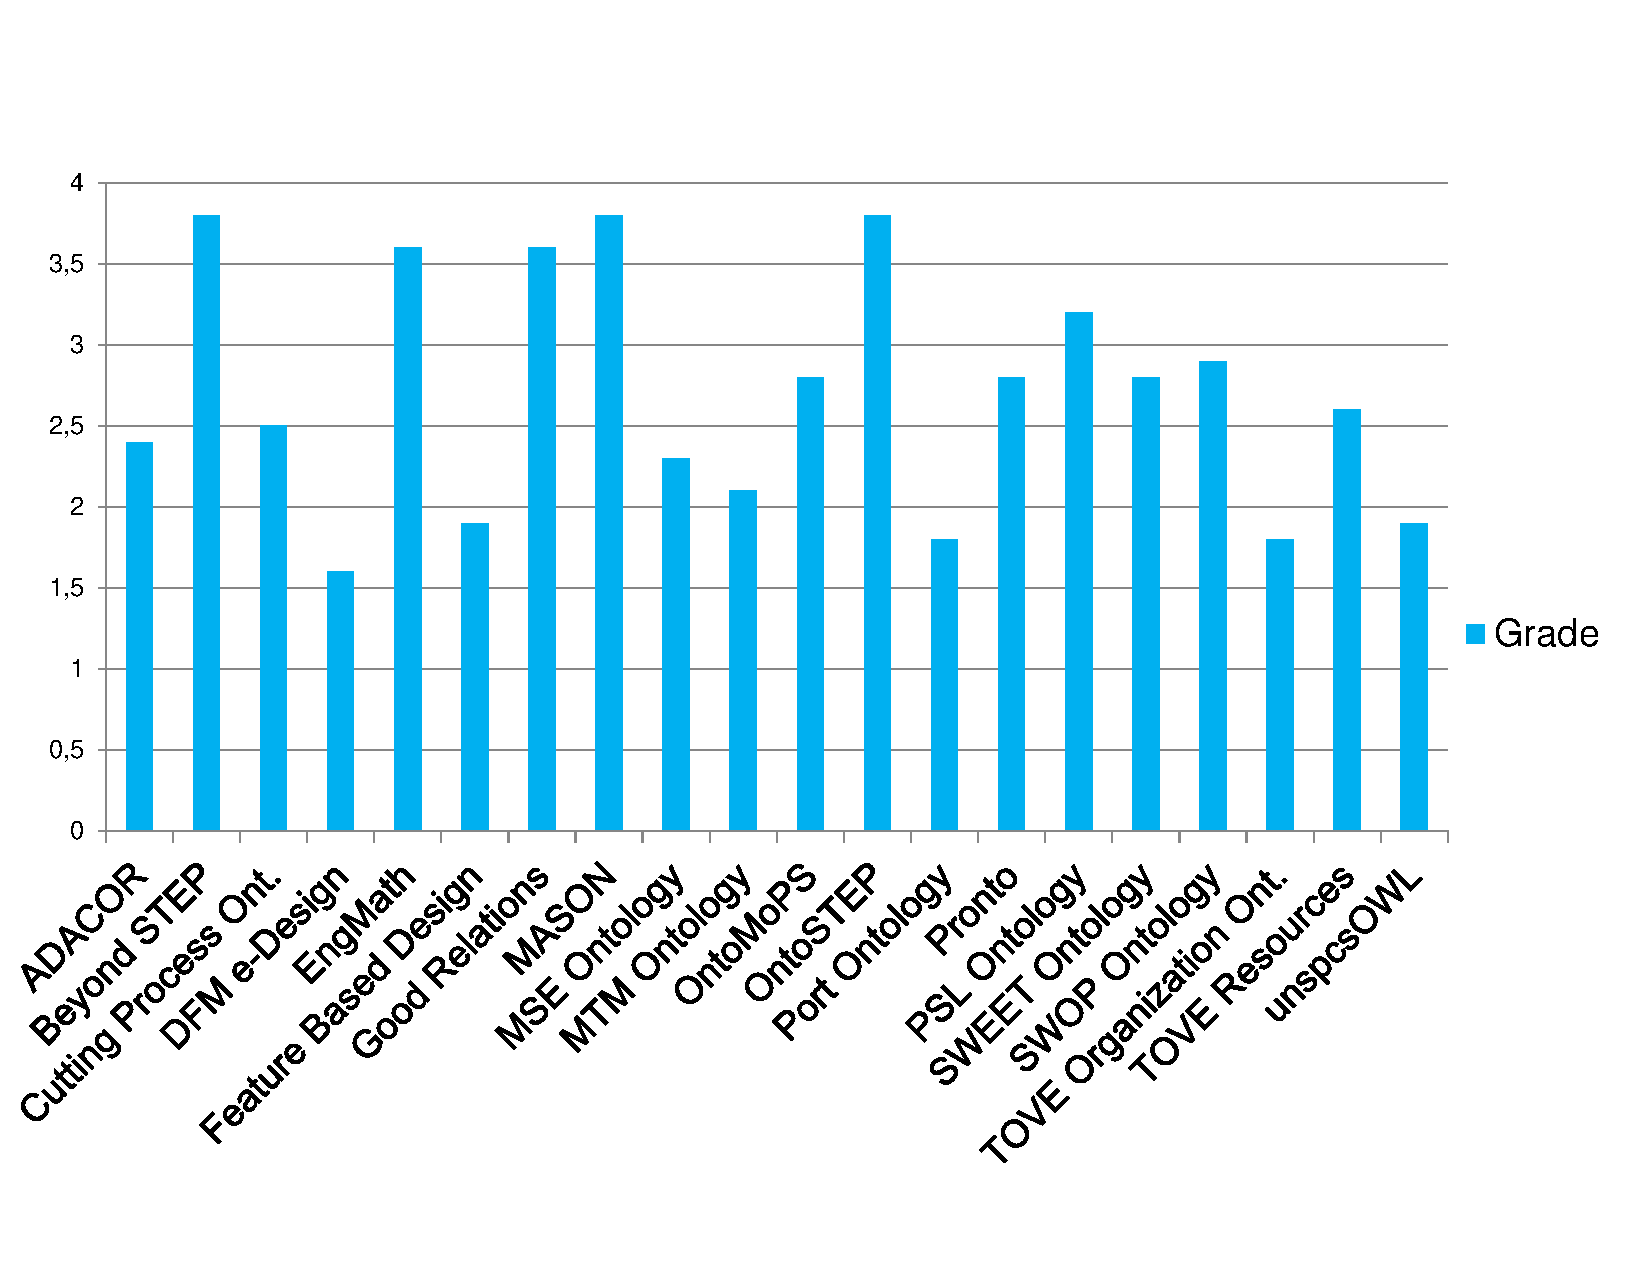
\includegraphics[scale=0.5]{figure-chapterIV/fig4-1.pdf}\\
		\caption{Results of Input Evaluation}
		\label{figure4-1}
	\end{center}
\end{figure}

The ontologies listed in Table \ref{table4.1} were submitted to the first quality assurance of Onto\textit{Smart}\footnote{shorturl.at/oBEIV}. In order to quantify those parameters we built and proposed a questionnaire\footnote{https://github.com/luisenriqueramos1977/OntoSmart/wiki/General-Informational-Quality-Evaluation-Questionnaire}. There, every dimension is presented with a list of weighted scenarios. The value of the scenario is ranging from 1 on an ideal situation to a lower value given to worse or less advantageous scenarios. The results of applying this questionnaire permitted us determine the current quality level of each ontology. Fig. \ref{figure4-1} outlines the output of performing this preliminary evaluation. 

According to the results shown here, Ontologies evaluated can be divided into three categories: those with a quality range [4, 3] were considered of high quality and passed to the next evaluation procedure. Ontologies with a quality range (3, 2] were considered of good quality and passed to the next stage. The ontologies within the range (2,0) were discarded.   


A simplified view of these quality sets mentioned above is outlined in Fig. \ref{figure4-2}. From this figure, it can be considered that a reduced number of ontologies fulfill the reusability criterion we proposed in the questionnaire.  That is 30\% appears as highly reusable, while a larger set can be reused   after certain intervention of the ontologists. A last set is of low quality and should not be reused. 


\begin{figure}
	\begin{center}
		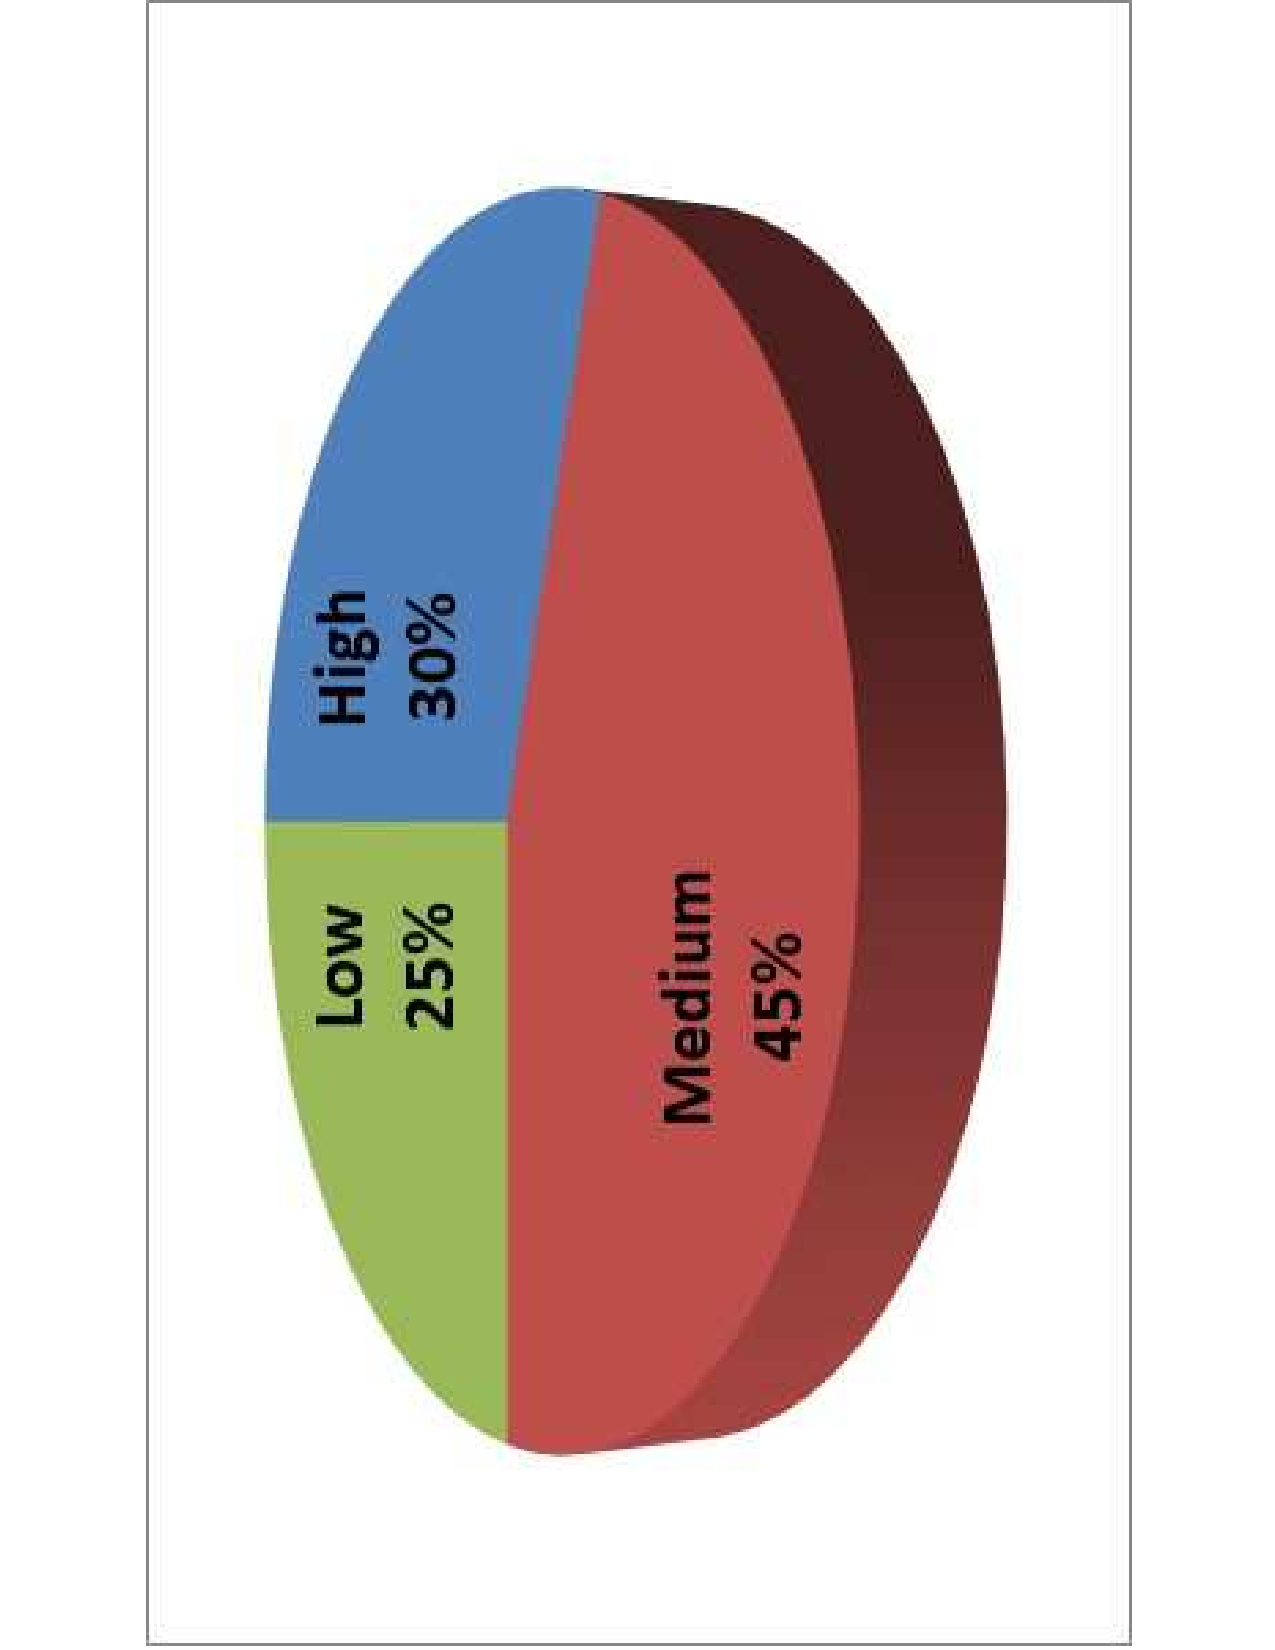
\includegraphics[scale=0.4, angle=-90]{figure-chapterIV/fig4-2.pdf}\\
		\caption{Grouping of Ontologies by Quality Level}
		\label{figure4-2}
	\end{center}
\end{figure}



Reasons leading to a larger set of low and medium quality ontologies are displayed in Fig. \ref{figure4-3} and Fig. \ref{figure4-4}. Firstly, conceptually speaking, ontologies should be publicly available, and with minimum limitations for their use.  However, as Fig. \ref{figure4-3} shows, from our sample ontologies, only 55\% were available for direct download or provided by authors, while the other portion was not. This issue limits the use of an ontology and also reduces the possibility of performing a more accurate evaluation. 


\begin{figure}
	\begin{center}
		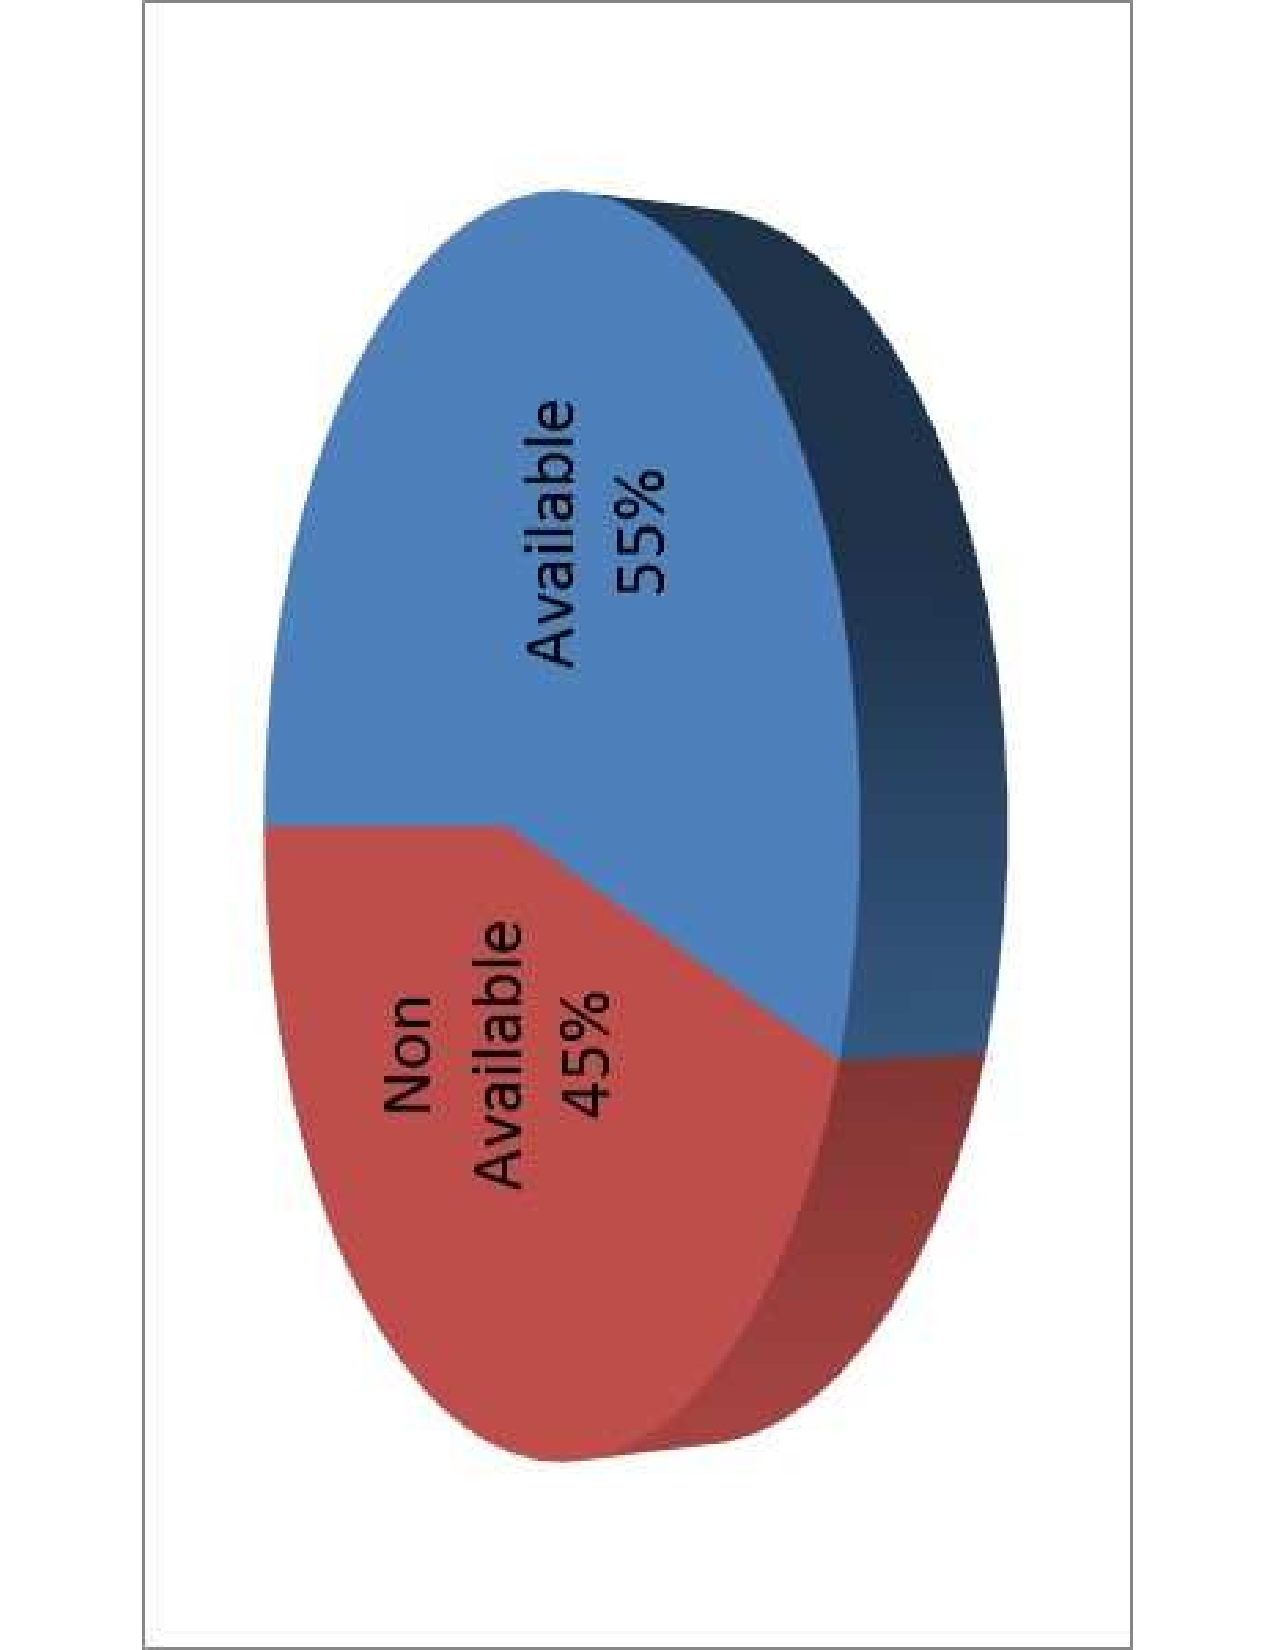
\includegraphics[scale=0.4, angle=-90]{figure-chapterIV/fig4-3.pdf}\\
		\caption{Ontology Availability Evaluation}
		\label{figure4-3}
	\end{center}
\end{figure}



Furthermore, as the next figure shows, explicit indication of rights to reuse and modify the ontology had also been omitted in most of the reviewed ontologies. In an ideal situation, this legal statement should be encoded within the ontology itself, and in the worst case, it should be specified on the site where an ontology is available for download. \gls{owl} has a mechanism that makes it possible to add such types of annotations to ontologies, but even in many of the ontologies written in \gls{owl} this possibility was not used.

Finishing this first evaluation procedure, ontologies were reordered according to the quality level previously given. Table \ref{table4.2} lists the order in which ontologies will be considered for subsequent uses and evaluation. 



\begin{figure}
	\begin{center}
		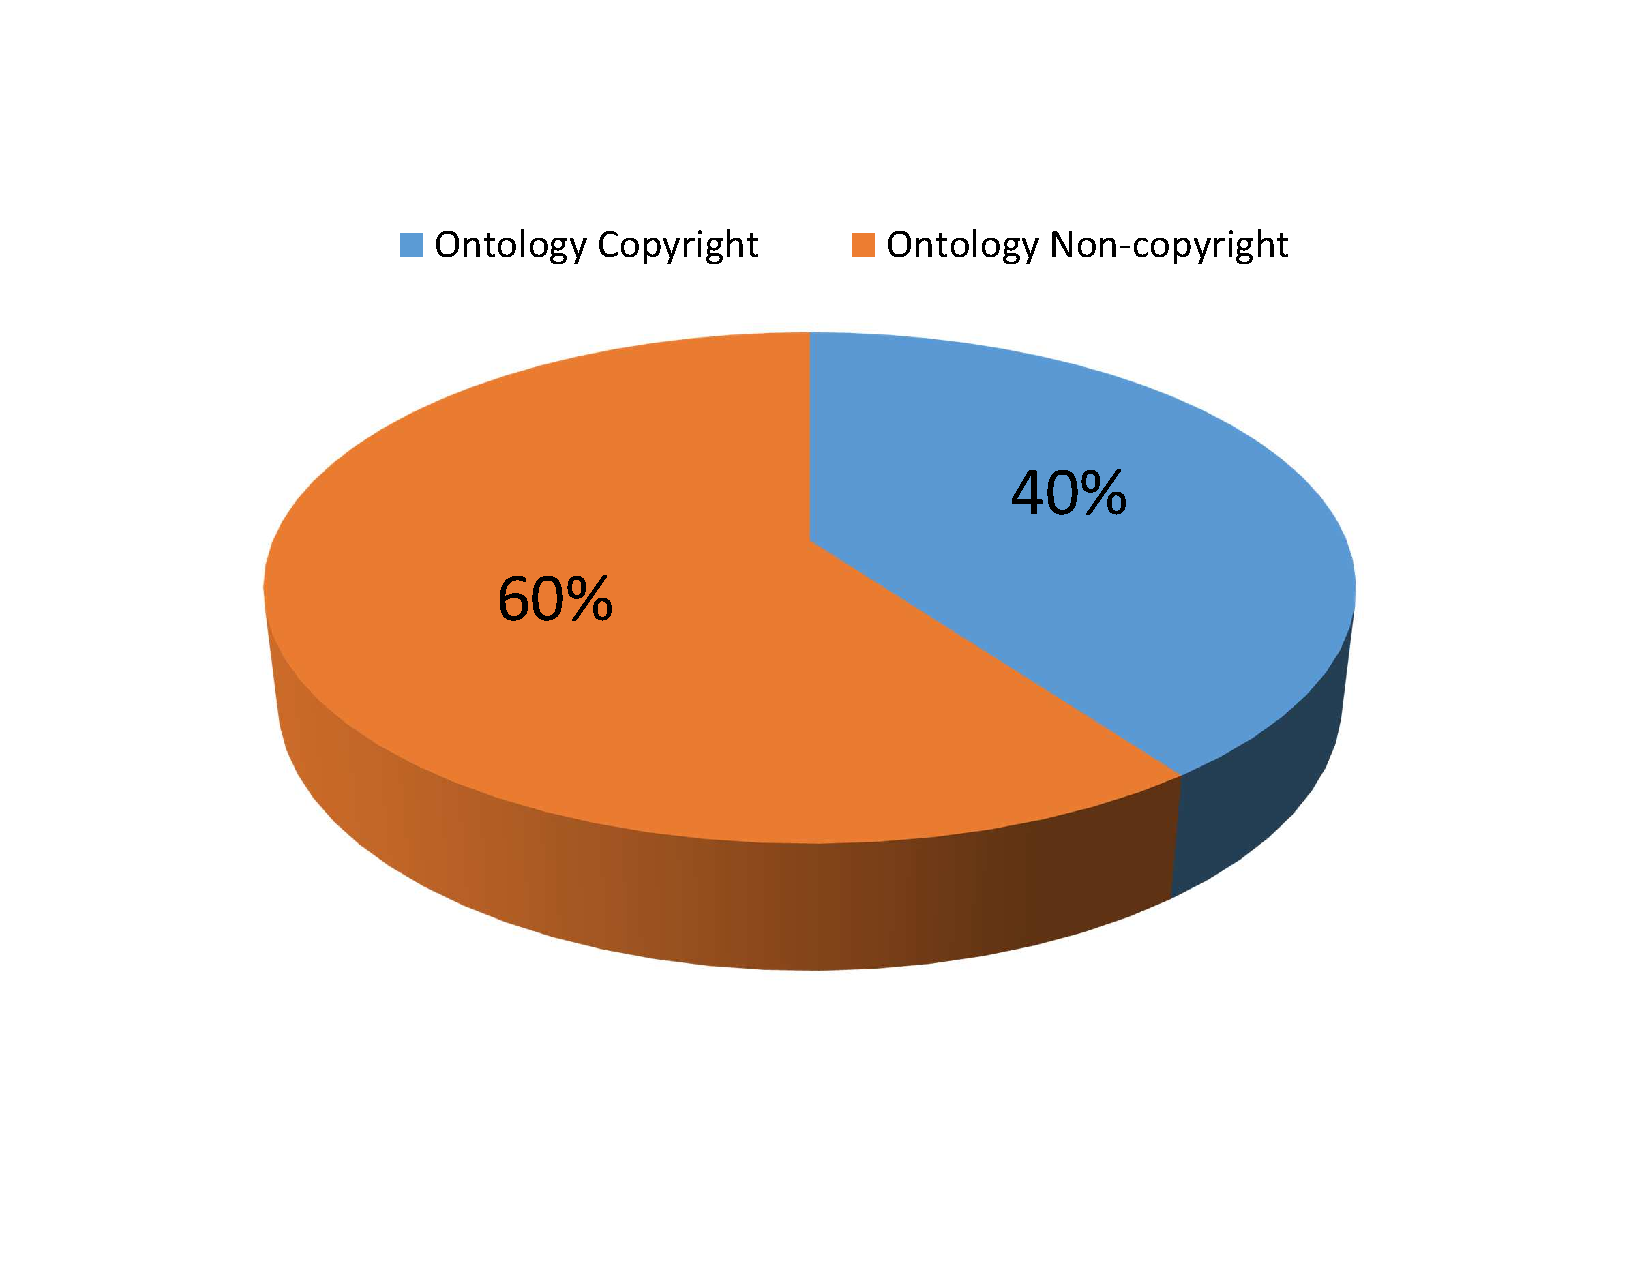
\includegraphics[scale=0.4]{figure-chapterIV/fig4-4}\\
		\vspace{-20mm}
		\caption{Ontology Intellectual Property Evaluation}
		\label{figure4-4}
	\end{center}
\end{figure}






\begin{table}[tp]%
	
	\caption{Quality Order}
	\label{table4.2}\centering %
	\begin{tabular}{cl}
		\toprule %
		Quality Order &	Ontology Name (Acronym) \\\toprule
		
		\textbf{1}&	\textbf{\gls{mason}} \\\toprule
		\textbf{1}&	\textbf{Beyond STEP Ontology}\\\toprule
		\textbf{1}&	\textbf{OntoSTEP}\\\toprule
		\textbf{2}&	\textbf{GoodRelations}\\\toprule
		\textbf{2}&	\textbf{EngMath}\\\toprule
		\textbf{3}&	\textbf{\gls{psl} Ontology}\\\toprule
		4&	SWOP Product Ontology \\\toprule
		5&	SWEET Units\\\toprule
		5&	\gls{pronto}\\\toprule
		5&	ONTOMoPS\\\toprule
		6&	Resource Ontology (TOVE)\\\toprule
		7&	Cutting Process Ontology\\\toprule
		8&	ADACOR\\\toprule
		9&	MSE\\\toprule
		10&	MTM Ontology\\\toprule
		
		
		
		
	\end{tabular}
	
	
\end{table}



\subsection{Performing Competency Questions}\label{subsection4.2.3}

The use of Competency Questions to define the scope of ontologies, and additionally to validate them, was explained in Section \ref{methodology}. This technique was included as a part of the proposed methodology.   Therefore, in Subsection \ref{4.1.2} a set of competency questions for the manufacturing domain was proposed. Here we mention that if one of the ontologies listed in  Table \ref{table4.2} provides appropriate answers to all Competency Questions, then we can proceed to hosting and implementing that ontology as given in our proposed methodology presented in Section \ref{methodology}. However, if no ontology fulfills this requirement, then this will require developing a newer ontology, although preferably reusing existing content.  

Competency Questions were performed on the \gls{owl} ontologies listed in Table \ref{table4.2} considering their quality order, specifically ontologies  with a quality order in the range from 1 to 3. The Query Tab plugin of the ontology editor Protégé was chosen from Table \ref{table1}. This choice was made because, first both the editor and the Plug-In support \gls{owl}, and second because they offer a friendly interface that makes interaction with the chosen ontology possible.  To illustrate this example we chose \gls{cq}3 (Section \ref{4.1.2}), which in natural language is expressed as follows: which machinery enables the realization performance of a given manufacturing operation? It is worth  mentioning that this query is concatenated with \gls{cq}2, which asks questions on product features. Furthermore, \gls{cq}3 can be considered as part of the context of scenarios 1 and 3 described in Section \ref{4.1.1}. In Equation \ref{eq4.1}, this query is formalized with \gls{sqwrl}.

\begin{equation}\label{eq4.1}
	Machine\_Resource(?m) \wedge enablesRealizationOf(?m,``punching") \longrightarrow sqwrl:select(?m,``punching")
\end{equation}


Fig. \ref{figure4-5} illustrates interaction with the ontology. That is, starting with the first ontology presented in Table \ref{table4.2}, that is the \gls{mason} ontology, our chosen ontology was manually populated with data. That means, several instances of the concept \texttt{mason:Machine\_resource} were created, and properties of machines were encoded in the ontology, using information of commercial brochures. In this example, a \texttt{mason:Machine\_resource} was related to a  \texttt{mason:Punching} operation by  a \texttt{mason:enablesRealizationOf} predicate. The Query Tab presented in Fig. \ref{figure4-5} is organized according to Protégé vocabulary, therefore from left to right we can view the terms “Class” which is a concept (\texttt{mason:Machine\_resource}), the term “slot” corresponds to a predicate or property (\texttt{mason:enablesRealizationOf}), and the condition “contains”. Within “contains” we will evaluate wheter or not a concept contains a given individual. The resulting individual has to satisfy the condition drawn by the query. In this case the query evaluates whether or not the given instance is “contained” by any individual in the target class by means of a property. In the illustrated case it was possible to find an instance that fullfils our requirement, that is the individual \texttt{mason:Punching\_press}. The result is shown on the right of the figure in “Search Result”. In natural language we can say that we found machinery that enables performance of punching operations, which is a Punching Press. In other words, we found a result for our query. This procedure was followed with every ontology of Table \ref{table4.2}


\begin{figure}
	\begin{center}
		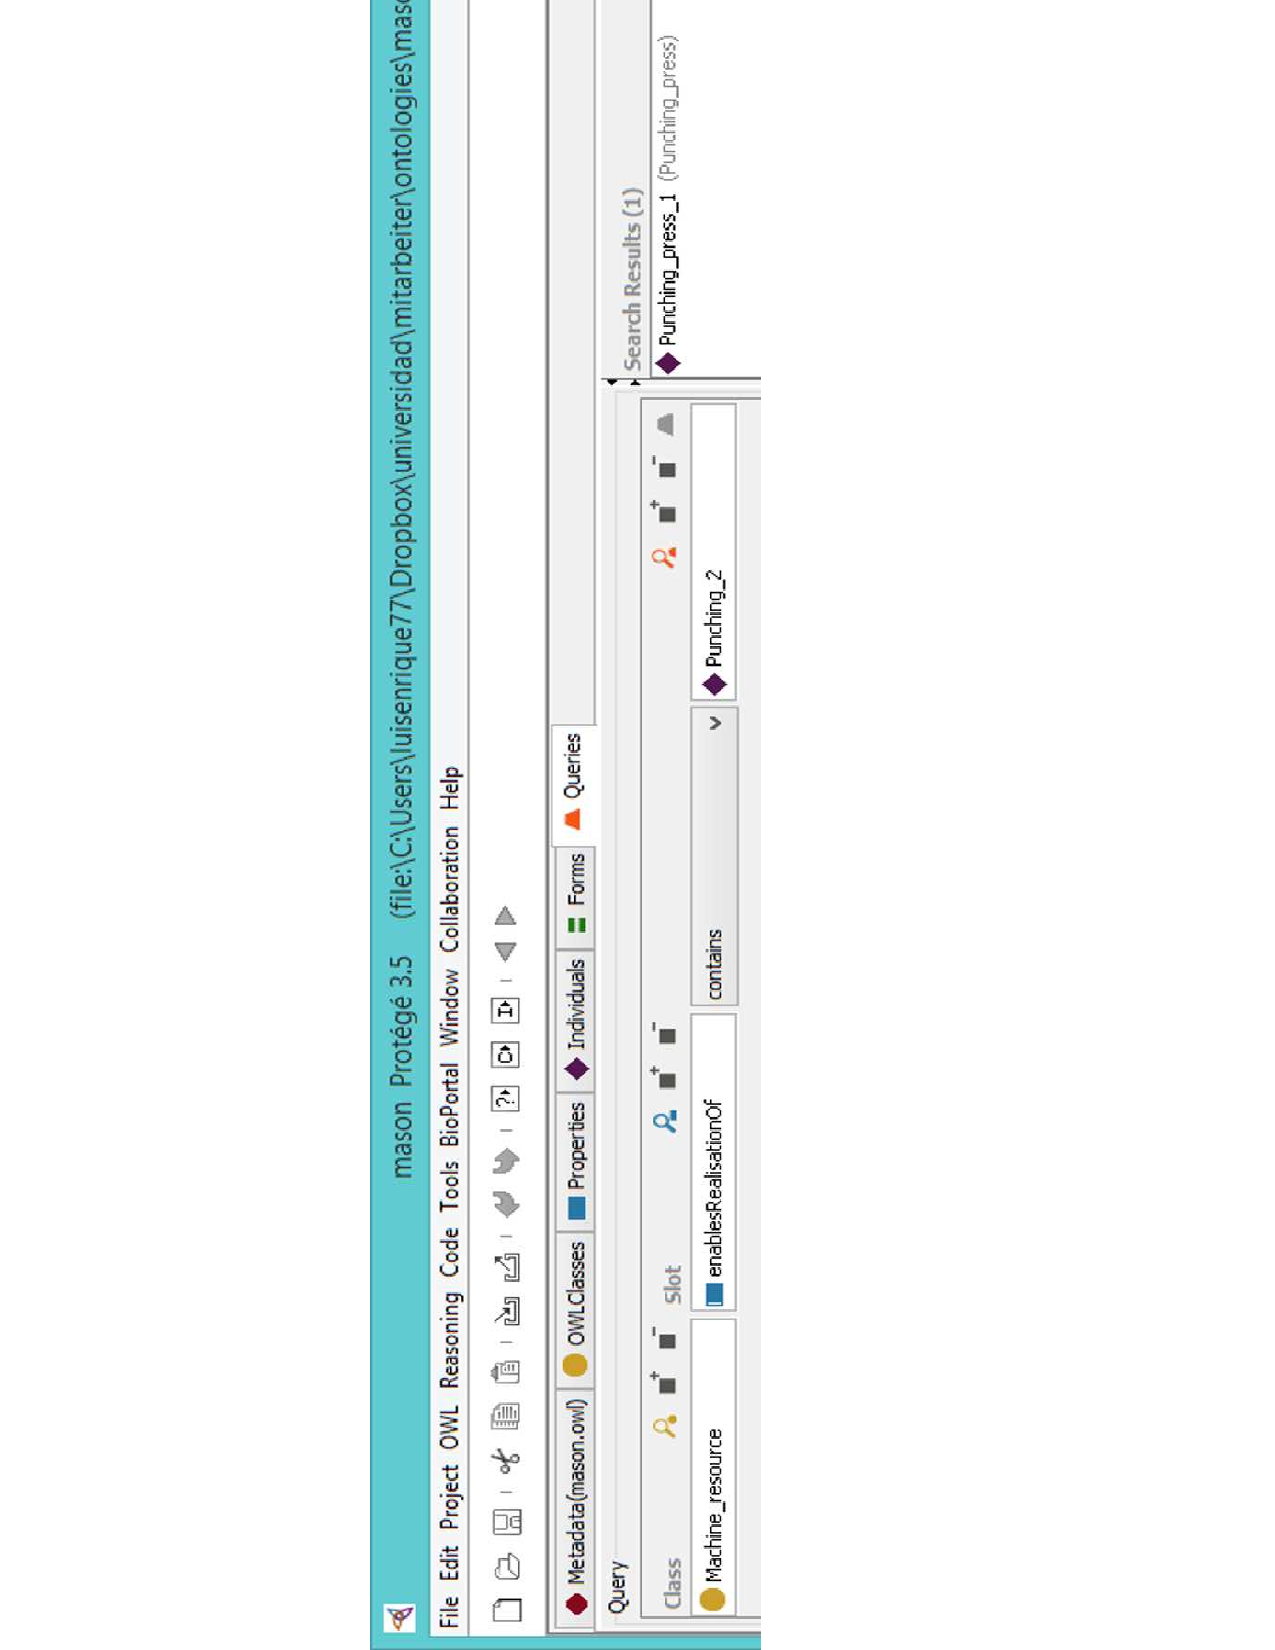
\includegraphics[scale=0.8]{figure-chapterIV/fig4-5}\\
		\caption{Ontology Query in Protégé}
		\label{figure4-5}
	\end{center}
\end{figure}


\begin{equation}\label{eq4.2}	
	\begin{split}
		(defrelation is-occurring-at (?punching ?p) := \\
		(and (activity-occurrence ?punching) \\
		(betweenEq (beginof ?punching) ?p (endof ?punching)))) 
	\end{split}
\end{equation}\\

For ontologies written in other languages (\gls{fol}, \gls{kif}), questions were considered as answerable when the available terminology (concepts and predicates) could be structured to represent the requirement expressed in the query. For instance,   within \gls{cq}7 it is required to answer whether or not an operation or activity is occurring in a given time space. This can represented in \gls{psl} as indicated in Equation \ref{eq4.2}. In \gls{psl} vocabulary an \textbf{activity-occurrence} or manufacturing operation \textbf{is-occurring-at} a timepoint \textbf{p} if and only if \textbf{p} is \textbf{betweenEq} the activity occurrence’s begin and end points.\gls{psl} therefore supports the required representation of \gls{cq}7, and within it we can confirm if a given activity is taking place.



Fig. \ref{figure4-6} shows how many competency   questions were answered by each ontology, according to the procedure described above. 



\begin{figure}
	\begin{center}
		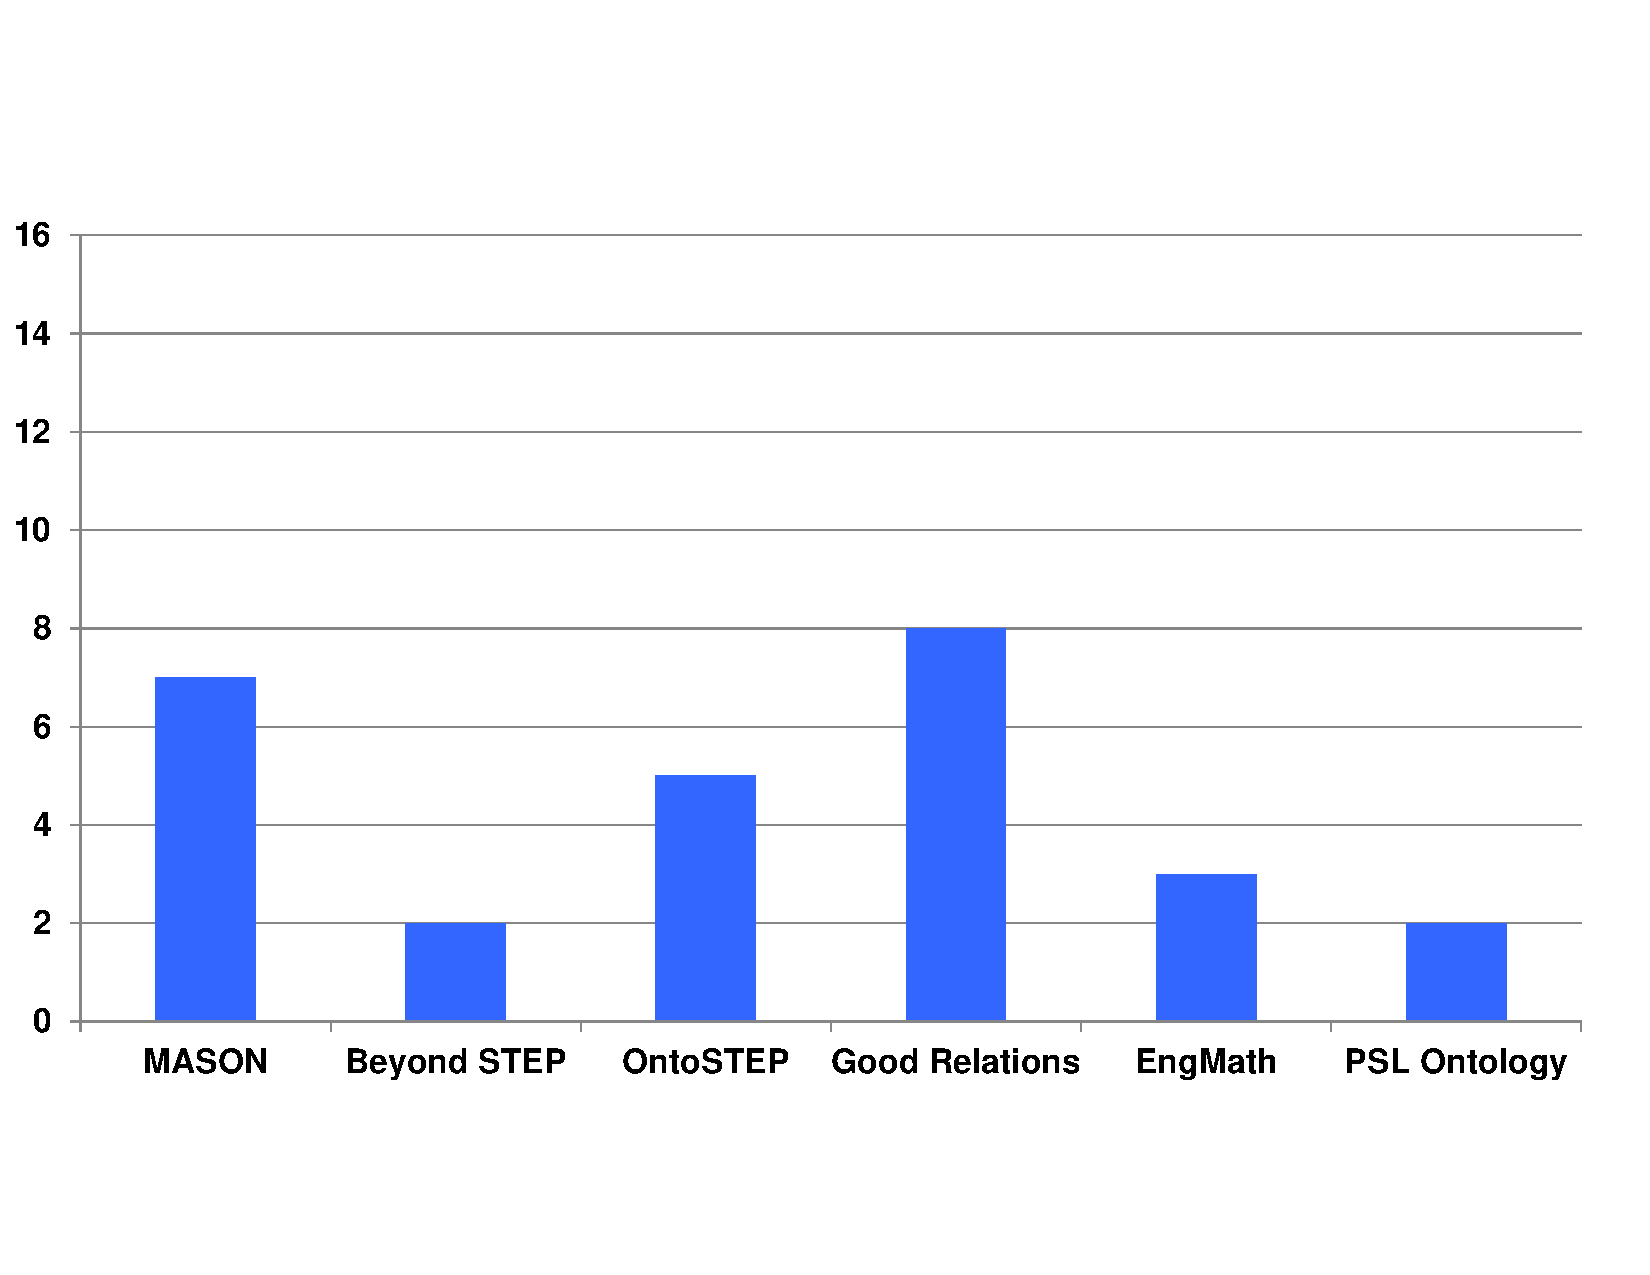
\includegraphics[scale=0.5]{figure-chapterIV/fig4-6.pdf}\\
		\caption{Queries Answered per Ontology}
		\label{figure4-6}
	\end{center}
\end{figure}



If we want to use the number of competency questions answered per ontology as a quality parameter, it could be considered that the quality of selected ontologies is low because most of them represent a quantity of knowledge only sufficient to answer less than 50\% of the questions. Nevertheless, within Fig. \ref{figure4-7} a distributed view can be presented. This graphic breaks down how the selected ontologies \textit{as a whole} provide answers to 15 of 16 queries. Every column represents the number of ontologies that provide adequate answers to the corresponding \gls{cq}. For instance, no ontology provides an answer to \gls{cq}-3, while \gls{cq}-2, \gls{cq}-6 and \gls{cq}-9 found answers from three different ontologies respectively. 


\begin{figure}
	\begin{center}
		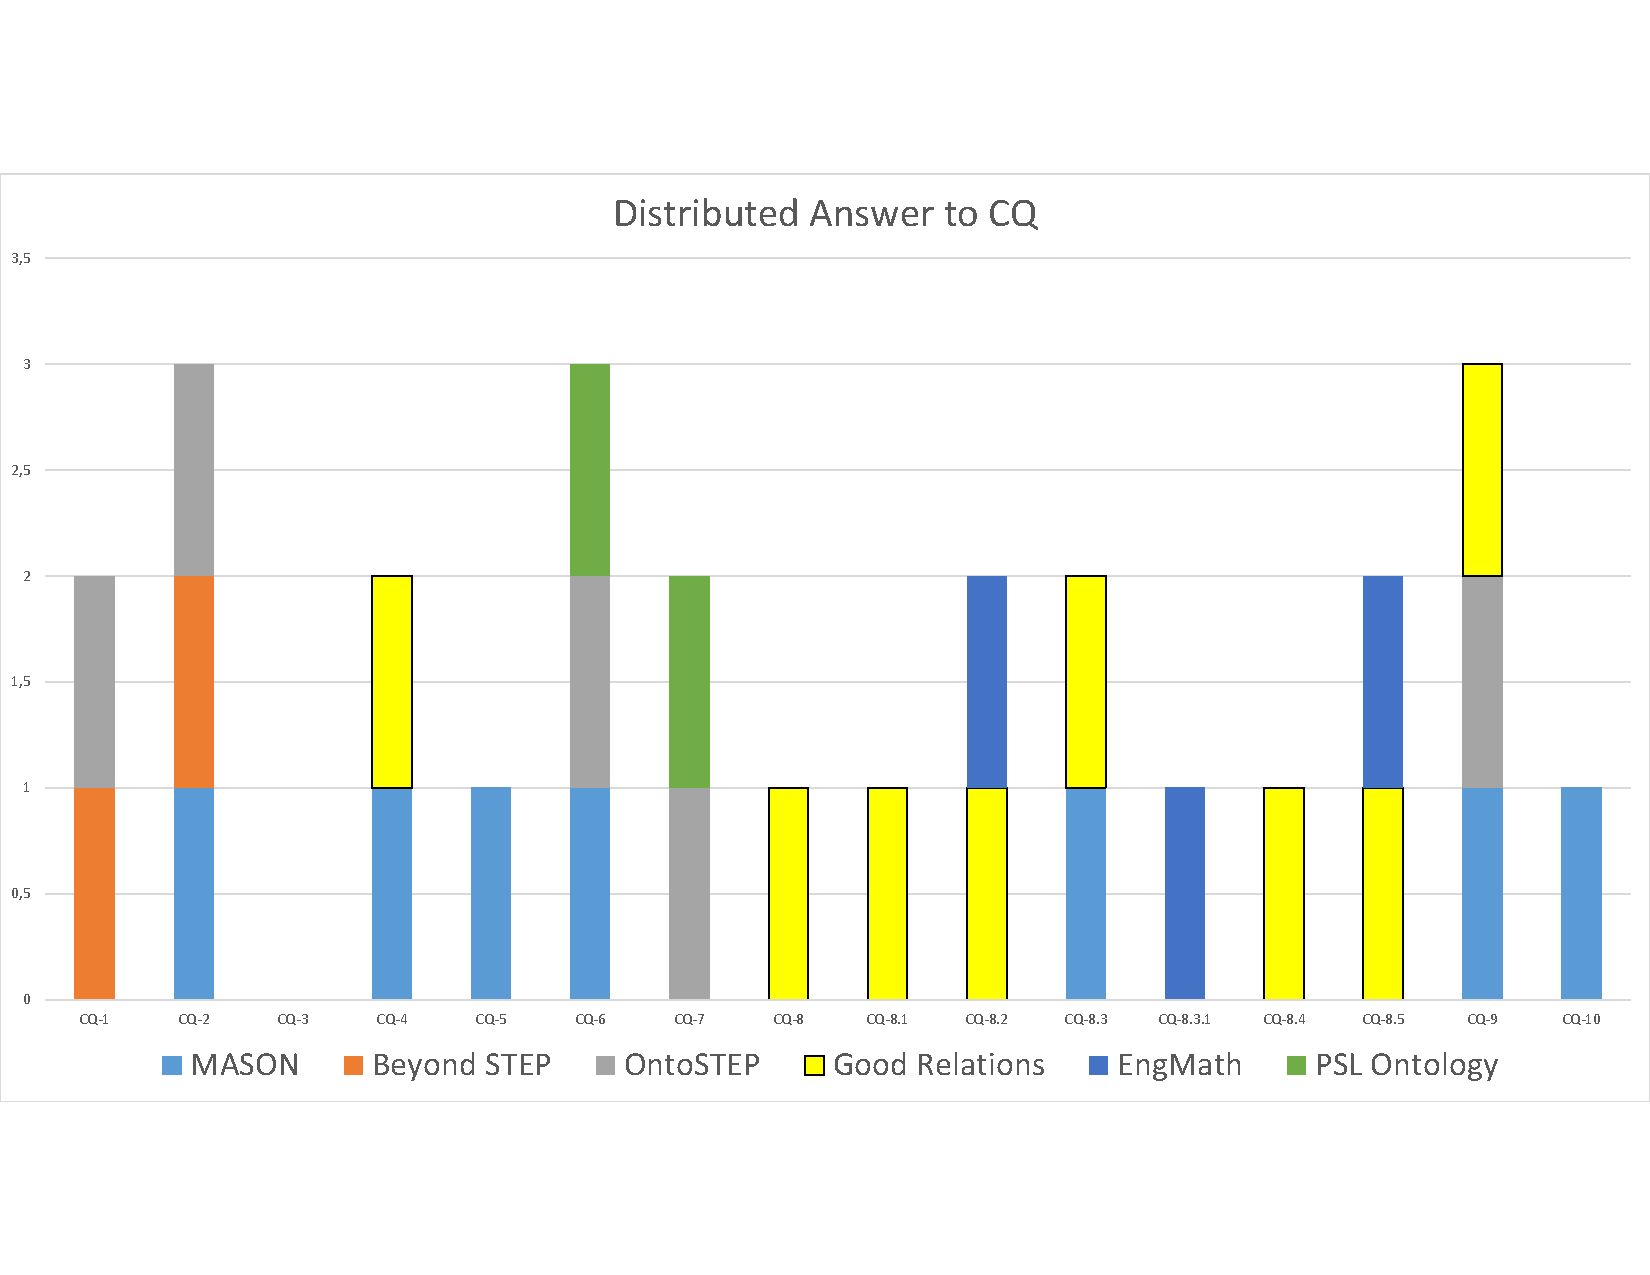
\includegraphics[scale=0.5]{figure-chapterIV/fig4-7}\\
		\caption{Answers Distribution between Ontologies}
		\label{figure4-7}
	\end{center}
\end{figure}



From our point of view, answers to these \gls{cq} certainly support using \textit{modularity}. That means working with a network of ontologies we can be more efficient in the sense of getting more answer to our \gls{cq}'s than working with individual ontologies. In other words, while there is no ontology that provides answers for every \gls{cq}, many \gls{cq} can obtain answers from different ontologies. That means working with these ontologies in a modular architecture, we can obtain answers to 94\% of the given queries, while just using such ontologies alone we would be able to provide answers to only 50\% of the \gls{cq}. 

In fact, more than obtaining an answer for most queries, several ontologies provide an answer to related sets of queries, while many others can be divided into those where the ontology provides an answer to only one query, and others that do not provide answers to any other query.  Such an outcome indicates that, on  the one hand, there is some common knowledge between these ontologies, and it would be possible for a question to obtain answers from different ontologies. On the other hand, there are some questions that obtain answers only from one ontology, indicating that there is certain localized and isolated knowledge in some of them as well. 


\begin{figure}
	\begin{center}
		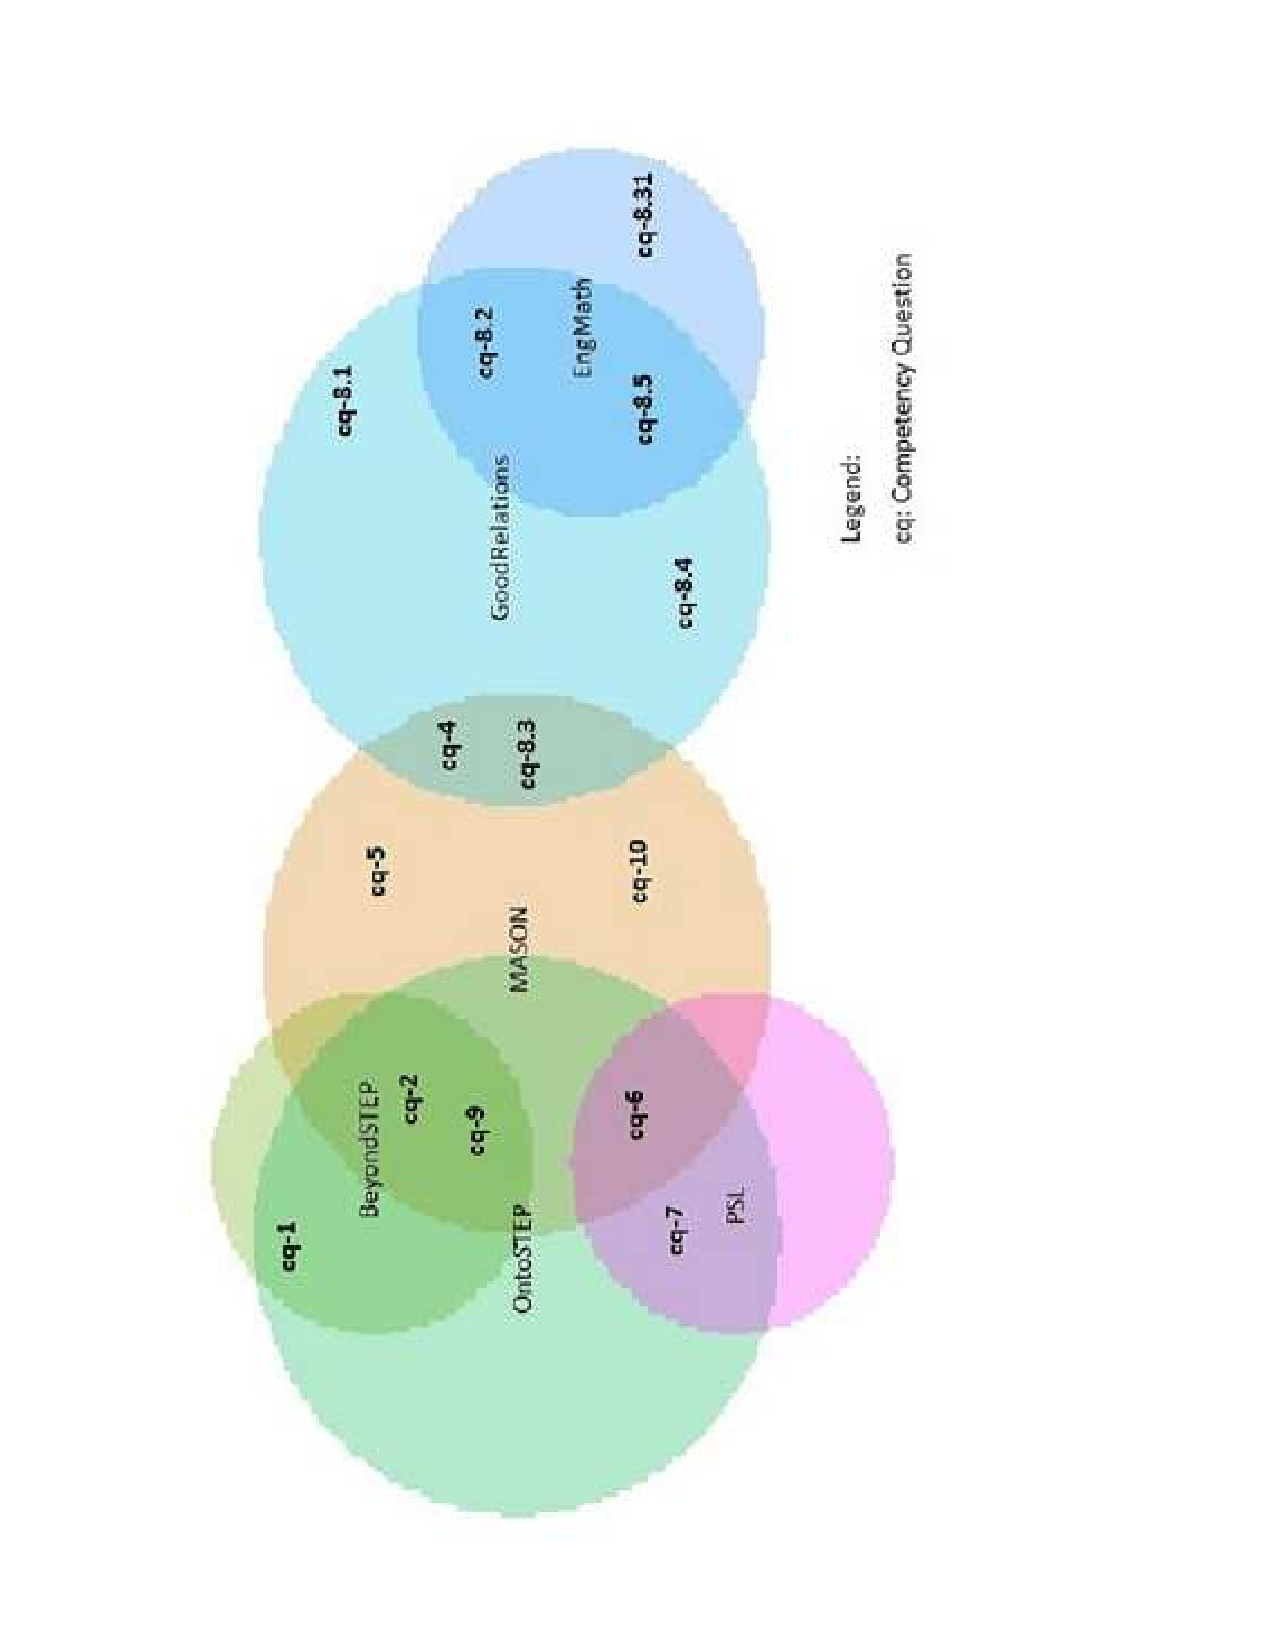
\includegraphics[scale=0.8]{figure-chapterIV/fig4-8}\\
		\caption{Ontological Commonalities in Answers to Competency Questions}
		\label{figure4-8}
	\end{center}
\end{figure}



Fig. \ref{figure4-8} represents another view of the scenario described in the previous paragraph. There, every circle represents one ontology and their overlapping regions indicate commonalities in answers to \gls{cq}s. The position of circles in this figure is also meaningful: from the middle to the left side, there are ontologies related to the products represented as solid   parts, and the manufacturing process representation as well. OntoSTEP nearly subsumes BeyondSTEP and \gls{psl} has commonalities with OntoSTEP and \gls{mason}, but not with BeyondSTEP. This occurs because BeyondSTEP does not mention any process in its terminology. On the right side of this figure is GoodRelations. This ontology is intended to represent products on the Internet, but it does not deal with representing manufacturing processes, therefore it is isolated from \gls{psl}. While it holds some relation with queries that can be answered by EngMath, given that the former highlights the use of International System  Units   in the definition of product features and parameters, which is wthin the scope of EngMath. For instance, in the case of the \gls{cq}-8.5 \textbf{What is the replacement cost?}, which is a query that comes from the fields of cost accounting, projects evaluation and insurance, concepts related to monetary units and physical units are required. Thus, for \gls{cq}-8.5 the concepts \texttt{gr:UnitPriceSpecification}, \texttt{gr:QuantitativeValue} (GoodRelations), and \texttt{system-of-unit} (EngMath) can e considered to provide an appropriate answer to this query. We can also mention that this result differs from what would be expected from ontologies for manufacturing and engineering science in general, given that metric units, the definition and concepts are fundamental in these fields. However, metric concepts do not appear in most of them.


In order to continue with this subject, and to provide sufficient generalization, it is beneficial to make use of Onto\textit{Smart}'s definitions\footnote{https://github.com/luisenriqueramos1977/OntoSmart/wiki/Formal-Definitions}.

Definition 4\footnote{shorturl.at/kBLNZ} can be visualized in Fig \ref{figure4-8}, where a modular domain was obtained. 

In this case, considering the definitions proposed in Onto\textit{Smart}, and the results obtained until now, which are represented as the number of answer to queries (see Fig. \ref{figure4-6} and Fig. \ref{figure4-7} and its distribution in the network of ontologies  (see Fig. \ref{figure4-8}) we can proceed to summarize our findings in order to decide which way to  go from here:

\begin{enumerate}
	
	\item 	First, according to the results outlined in Fig. \ref{figure4-6}, where we can see no ontology provides answers to every \gls{cq}, a fully reusable ontology $o_{r}$, as defined in Definition 3\footnote{shorturl.at/alyH0} of Onto\textit{Smart}, is not present in the manufacturing domain under study, and so a direct step to implementation is not possible for the given use case.   \label{it1} 
	
	\item Second, development from scratch should be discarded, given that the current manufacturing ontologies under consideration provide enough information to answer most of the domain questions  listed in Section \ref{4.1.2}, as we can observe in Fig. \ref{figure4-6}. Therefore, discarding these ontologies would make us lose time and other resources that could be used in developing a new ontology. \label{it2}
	
	\item Third, developing a new ontology with the ones evaluated as parts is another possibility. This ontology is also likely to use one of the existing ontologies as subsumed   and increase the knowledge encoded in the former by integrating the latter within it. \label{it3}
	
	\item Fourth, finding one ontology to be used as an interoperability artifact between a set of ontologies would make it necessary to determine whether an ontology exists that could be categorized as an upper level ontology. The use of this ontology should be similar to that displayed in Multiontology\footnote{https://github.com/luisenriqueramos1977/OntoSmart/wiki/Multiontology} Building Block of Onto\textit{Smart}, where one ontology is used with the sense of providing interoperability among domain ontologies. \label{it4}
	
	\item  Last, it is also possible to have separate ontologies that contribute to providing modeling structures and answers to queries distributed among subdomains.   For instance, a scenario like the one depicted in Fig. \ref{figure4-8}, where answer to queries are distributed among several ontologies.  \label{it5}
	
\end{enumerate}

Option \ref{it3} corresponds to the most common approach adopted in Ontological Engineering, that is: enriching an ontology by importing or merging other ontologies into it. Options \ref{it4} and \ref{it5} correspond to two schools of thought in Ontological Engineering. The former corresponds to the upper level approach, and the latter corresponds to the hyper-ontological approach. In the next subsection these approaches, their implementations and issues within our domain of study are discussed.


\subsection{Mapping, merging and importing}\label{subsection4.2.4}

In this Subsection, we applied Onto\textit{Smart}\footnote{https://github.com/luisenriqueramos1977/OntoSmart/wiki/Hypermodules-Extractions} techniques to ontologies listed previously in Table \ref{table4.2}  in order to clearly define which of the scenarios described at the end of the previous section we are facing. In other words, we have to determine if there is an upper level ontology, or if we have a network of ontologies, such as a Hyperontology.

However, it is necessary to remark that these techniques are simple to implement when dealing with \textit{homogeneous} ontologies written in the same implementation language. In our case most ontologies presented in Table \ref{table4.2} are written in \gls{owl}. Consequently, there were only four ontologies available for immediate mapping of this type; these were \gls{mason}, the BeyondSTEP Ontology, OntoSTEP and GoodRelations. The other high quality ontologies listed in Table \ref{table4.2}, \gls{psl} and EngMath, were not considered for automatic mapping because of its technological  limitation just mentioned, meaning that the ontology language of implementation differs from the language used in most high quality ontologies (\gls{owl}). 

According to the software tools listed in Table \ref{table1}, Protégé (prompt), Falcon and NeonToolKit are ontology editors that support \gls{owl}, thus they were chosen for mappings. Ontologies were mapped by pairs with every tool. The number of positive mappings were counted and tabled. Table \ref{table4.3} shows how this mapping experiment took place and which results were obtained by mapping the ontologies with different mapping tools and specific mapping techniques. In the third column mappings obtained by the PromptTab plug-in of Protégé are listed. In this case only mappings between pair of ontologies were found. In the other cases, no mapping was found.  The mapping experiment was repeated with Falcon. In column four results mapping the target ontologies are listed. Experimenting with Falcon, mappings were found in only one of six cases. 

A third mapping experiment was carried out by the NeonToolKit Alignment plug-in. The fifth column of Table \ref{table4.3} lists every time an alignment was found with this tool.  This time, unlike the previous experiments, a positive mapping was found for each pair of ontologies in most cases. There was a fundamental difference with this tool, that is we had the possibility to set up a similarity measure or threshold. Threshold of 1.0 would let us align only terms exactly written, a lower threshold value (e.g: 0.9, 0.8, 0.7) would let us align similar terms like \texttt{paint} and \texttt{painting}, but a low threshold value (e.g: 0.3, 0.2) could drive have to obtain wrong alignments of term like \texttt{paint} and \texttt{point}. Thus, for our experiments we chose to set up a  threshold of 0.7. As a result, mappings provided by NeonToolKit were considered for further analysis.

Although a performance evaluation of mapping is not in the scope in this research, it is worth remarking that different results were obtained by applying the different alignment algorithms available in each software tool. NeOn alignment plug-in provided the best results, thus these results were taken for working out the modularity.



\begin{table}[tp]%
	
	\caption{Number of Ontology Mappings through Different Tools}
	\label{table4.3}\centering
	\begin{tabular}{p{2.5cm} p{2.5cm} p{2.5cm} p{2.5cm} p{2.5cm} }\toprule
		
		Ontology 1 &	Ontology 2	& Protégé 3.4.4 PromptTab*
		(Number of Alignments)	&Falcon-AO
		2010
		(Number of Alignments)	&NeonToolKit 2.3.1
		Alignment Plug in!
		(Number of Alignments) \\\toprule
		
		\gls{mason} &	BeyondSTEP&	18&	NaN	&34  \\\toprule
		\gls{mason} &	GoodRelations&	0&	NaN&	14 \\\toprule
		\gls{mason}	&OntoSTEP&	SC&	0,85&	101 \\\toprule
		BeyondSTEP&	OntoSTEP&	SC&	NaN&	209 \\\toprule
		BeyondSTEP&	GoodRelations&	0&	NaN	&21 \\\toprule
		OntoSTEP&	GoodRelations&	0&	NaN&	417 \\\toprule
		
	\end{tabular}
	\begin{flushleft}
		* With Lexical matching\\
		!SMOA Name Alignment and trim 0.7\\
		SC: System crashes \\
		NaN: No Alignment found\\
	\end{flushleft}
	
	
	
\end{table}

Mappings obtained with NeonToolKit (fifth column) were carefully checked manually in order to remove mappings that we considered incorrect, thus    \gls{fp} mappings produced by the mapping system were removed and only \gls{tp} mappings were included \cite{oliver_kutz_chinese_2010}. The cleaning process consisted in discarding every mapping falling in each of the following cases:

\begin{itemize}
	
	\item Property–property mappings were discarded.  
	
	\item Redundant mapping through subsumption relations, in other words a concept in source mapped to two or more similar concepts in target. For instance, we obtained mappings  from \texttt{Bezier\_Curve} in source ontology to \texttt{Rational\_Bezier\_Curve} and \texttt{Bezier\_Curve} in the target ontology. That means, NeonToolKit provided two pairs of mappings: (\texttt{Rational} \texttt{\_Bezier} \texttt{\_Curve}, \texttt{Bezier\_Curve}) and (\texttt{Bezier\_Curve, Bezier\_Curve}). Thus, the first pair was discarded, and the second was considered.
	
	\item Similar names, but with different meanings, e.g, mapping of \texttt{Paint} in source to \texttt{Point} in target, were discarded.
	
\end{itemize}


Furthermore, mapped concepts with a threshold lower than 1.0, but with similar meanings, were left in the mapping file, e.g., \texttt{Thread} in source mapped to \texttt{Threading} in target. Then, the total mappings were divided in \gls{fp} and \gls{tp} as depicted in Table \ref{table4.4}. The  output datasets corresponding to this experiment are available online (adding a link - I will publish the link before delivering the thesis).  


\begin{table}[tp]%
	
	\caption{Ontology Mapping in Manufacturing Domain (First Iteration)}
	\label{table4.4}\centering
	\begin{tabular}{p{2.5cm} p{2cm} p{2.5cm} p{1.5cm} p{1cm} p{1.5cm}}\toprule
		
		Ontology 1 & Concepts in source Ontology &	Ontology 2	& Number & of & Mappings
		
		\\\cline{4-6}
		
		&	&	& \gls{fp} & \gls{tp} & Total  \\\toprule
		\gls{mason} &	222 &	BeyondSTEP  &	27 &	7&	34 \\\toprule
		GoodRelations&	37&	\gls{mason}&	14&	0&	14 \\\toprule
		OntoSTEP &	1625&	\gls{mason}&	90&	11&	101 \\\toprule
		BeyondSTEP	&114&	OntoSTEP&	104	&105&	209 \\\toprule
		BeyondSTEP  &			-&	GoodRelations&	21	&0&	21 \\\toprule
		OntoSTEP&	-&	GoodRelations&	414&	3&	417\\\toprule
	\end{tabular}
	
\end{table}





Fig. \ref{figure4-9} shows a graphical representation of the \gls{tp} mappings.  Only true positive mappings  between selected ontologies related to manufacturing are shown. This \gls{tp} was selected according to the criterion previously described with the intention of avoiding incorrect mappings. For instance, mappings of similar terms with different meanings, like point and paint. Similar mappings were considered as \gls{fp} and were discarded. In the figure, we can observe that the number of mappings from BeyondSTEP to OntoSTEP (105) appears to be the most significant one in this set of ontologies, but when the number of concepts of Beyond STEP (114) were considered, and compared against the number of \gls{tp} mappings, it can be observed that more than 92\% of the concepts in BeyondSTEP were present in OntoSTEP. This result shows a scenario similar to the one shown in Fig. \ref{figure4-8}, where BeyondSTEP was mostly subsumed by OntoSTEP.  


\begin{figure}
	\begin{center}
		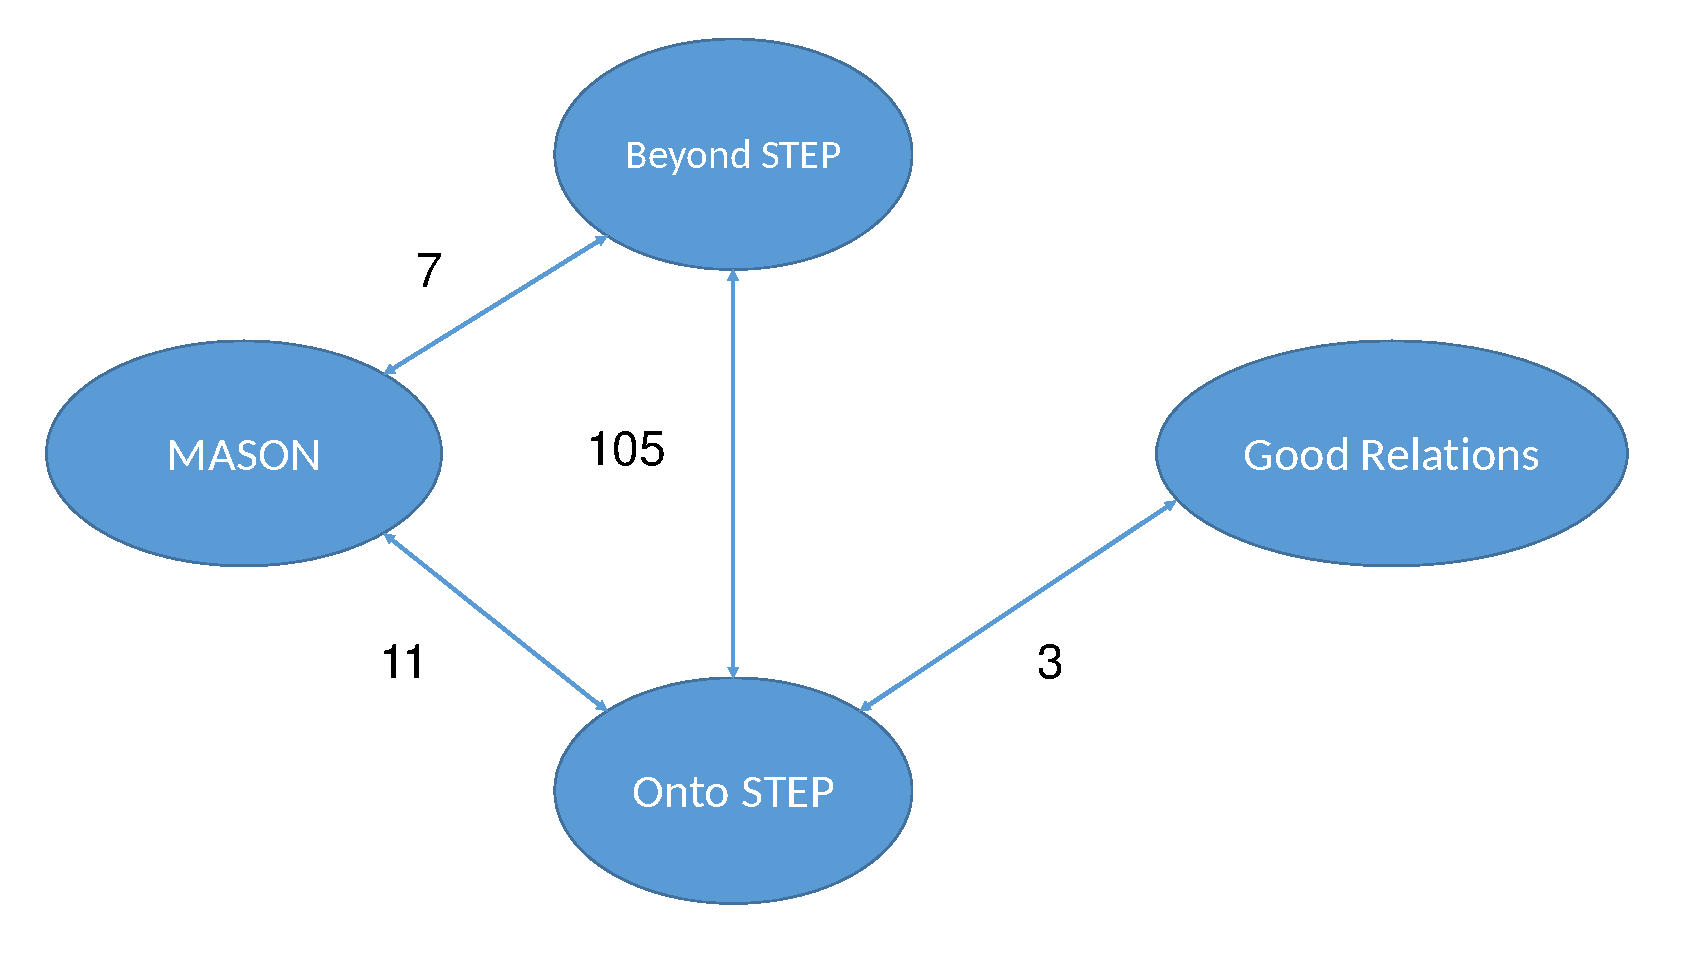
\includegraphics[scale=0.5]{figure-chapterIV/fig4-9}\\
		\caption{Ontological Commonalities in Answers to Competency Questions}
		\label{figure4-9}
	\end{center}
\end{figure}



However, when mappings are reviewed in detail, we find that both BeyondSTEP and OntoSTEP share some common mappings with \gls{mason}. These are the ones related to geometric concepts. Also, the mappings \gls{mason}-OntoSTEP highlight mechanical feature concepts on the one hand, while on the other hand the mappings   \gls{mason}-BeyondSTEP highlight more complex geometric concepts. This mapping situation shows a very common scenario in Ontological Engineering, i.e., the existence of    overlapping ontologies $O_{1}$ and $O_{2}$ which describe independent aspects of a given domain, but with some overlap. 

As our interest consists in finding answers to the competency questions previously listed, a first method would be to grant full access to the knowledge in those ontologies in order to answer these domain questions. This is equivalent to integrating them by merging. To proceed with this, Protégé 4 was selected from Table \ref{table1} as an ontology editor implementing support for merging ontologies. Thus, \gls{mason} and OntoSTEP were merged first, obtaining a new ontology. However, after merging them and running the respective reasoner, it was found that the resulting ontology became inconsistent.

Much has been studied about the issue   of inconsistency for ontology reutilization. For instance, \cite{ghilardi_did_2006} show that the appearance of inconsistencies when merging ontologies also depends on the logic of the ontology language in which the ontologies to be merged are implemented, in other words if we have two ontologies, one written in \gls{owl}, and another written in \gls{fol}, they cannot be merged, because of the language heterogeneity. To date some techniques to deal with inconsistent scenarios have been proposed by \cite{grau_owl_2008}  and \cite{xiang_ontofox:_2010}; both authors considered the need for user intervention and judgment in order to extract those modules from  $O_{1}$ which can be reused in $O_{2}$ avoiding inconsistencies. Others  authors have recommended keeping ontologies separated, but with logical links among these ontologies (e.g \cite{bateman_oasis_2009} and \cite{kutz_carnap_2010}). 

However, from the options given above, those considering human intervention are only feasible when dealing with pairs of small ontologies. In cases where a larger number of ontologies with a larger number of concepts are present, the implementation of appropriate algorithms for generating candidate modules is clearly going to be necessary as long as this proves possible.  Thus, the human intervention possibility is discarded here. Before considering the last possibility  (option \ref{it5}, of the list depicted in Subsection \ref{subsection4.2.3}, that is the  hyper-ontology), we exhausted option \ref{it4}: that is the possibility of finding one ontology of Upper Level as an interoperability artifact. Therefore, retaking Fig. \ref{figure3-1} where our methodology is described, we  decided on Reusability, because we found evidence that the ontologies under study (see Table \ref{table4.1}), provide answers to some of the proposed \gls{cq}, that means we are in a Multiontology environment. Then, we have to evaluate the most commonly found approach in Ontological Engineering, which is using an ontology as an interoperability artifact among other ontologies. That means that  we have to determine if one of the ontologies under study could receive  a higher categorization of upper level.   

In this vein the number of mappings in Fig. \ref{figure4-9} is insufficient to make any conclusions, because most of the mappings are inconsistent in number, and similarly directed to one ontology or distributed among ontologies. Therefore, a second mapping iteration   was carried out in order to obtain a larger network mapping, and obtain more accurate conclusions. 

According to the quality order previously outlined in Table \ref{table4.2}, the SWOP Product Ontology, SWEET Units, \gls{pronto} and ONTOMoPS were considered for this second iteration. In this case, only NeonToolKit was used for further experiences because of the better performance shown in the results obtained from Table \ref{table4.3} from the previous iteration. 

Fig. \ref{figure4-10} represents the output of including the mappings of this second iteration of ontologies. Here, OntoSTEP appears to also have the most mapping sets to every ontology in this network and BeyondStep has six mappings, while SWOP and OntoMoPs have five mappings respectively.  It is worth highlighting that these last two ontologies were not considered for the first iteration because of their lower quality evaluation. However with an automatic tool like NeonTooloKit we have found they have a large set of commonalities in the network of ontologies evaluated. The terms: \texttt{Product, Unit, Assembly, Process} and \texttt{Material} were some of those common terms found. SWOP and OntoMoPs were discarded at the begining because of preliminar evaluations, that did not consider the encoded knowledge in a first step. Those previous evaluation are ilustrated in Fig. \ref{figure4-1} and Fig. \ref{figure4-6}. Nevertheless, at this stage an automatic tool was included, taking us to discard others and retake these ontologies.




\begin{figure}
	\begin{center}
		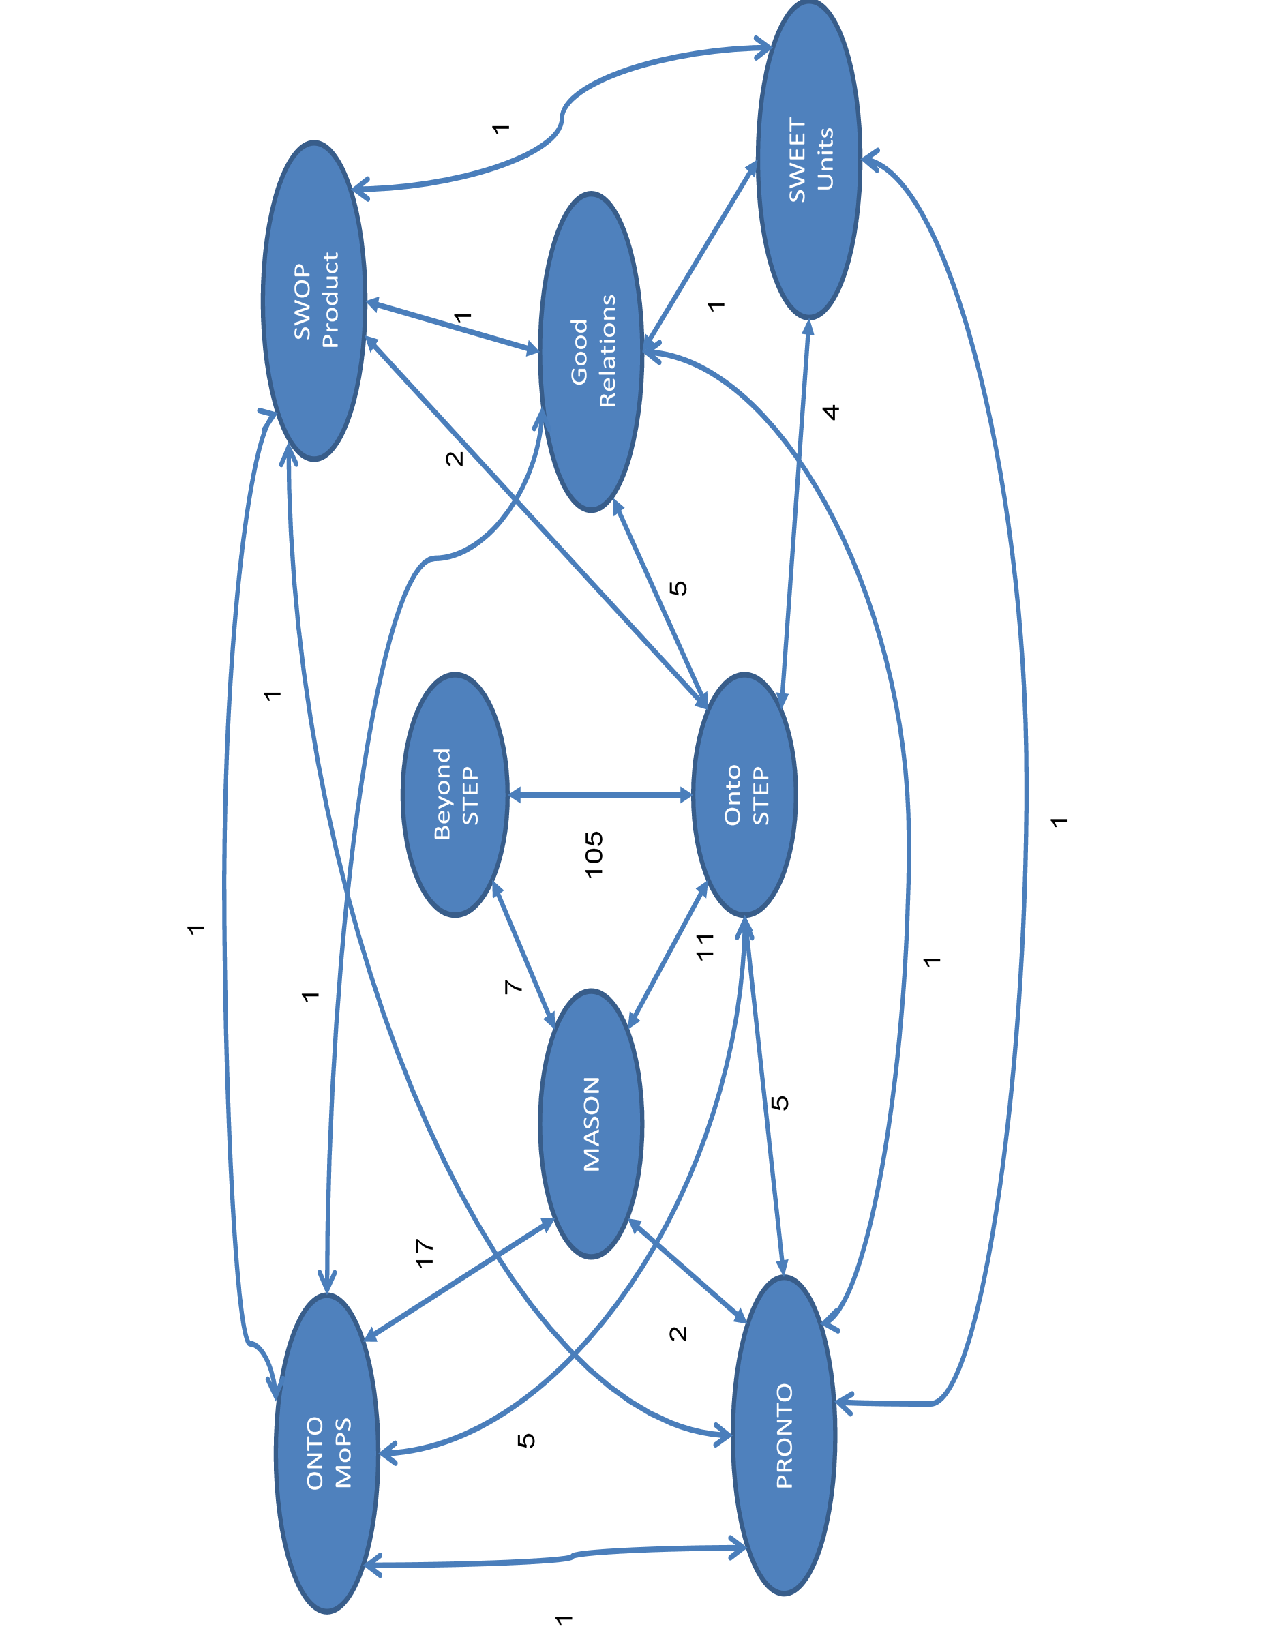
\includegraphics[scale=0.8]{figure-chapterIV/fig4-10}\\
		\caption{Network of Mappings in Manufacturing Ontologies}
		\label{figure4-10}
	\end{center}
\end{figure}



In the specific case of the set of mappings between BeyondSTEP and OntoSTEP, this large set of mappings was expected due to both ontologies having a closely related scope, which is the STEP standard. Although slightly different in the parts of the standard they modeled, the relation among the number of true positive mappings and the number of concepts of BeyondSTEP (92.1\%) allows us to affirm that BeyondSTEP is redundant compared to OntoSTEP.

Discarding the set of mappings between BeyondSTEP and OntoSTEP, a more complex scenario was obtained.  In this case, from the 28 mappings 19 were sets of true positive mappings ranging from only one (7 times) to 16 individual mappings. The sets of only one mapping contained the terms Product and/or Unit. The remainder sets contained terms related to geometry features of products, mechanical features, and other terms repeated less frequently, such as assembly, material and process. Table \ref{table4.5} presents the details of those terms and their frequency. Here we can retake the list of terms we mentioned in Section \ref{4.2.1}, proposed by \cite{martin_design_2003} and \cite{lastra_ontologies_2009} as significant for the manufacturing domain. Those  are \texttt{Product}, \texttt{Process}, \texttt{Resource} and \texttt{Equipment}. All of them except \textbf{Equipment} are present in this table. The obtained mapping terminology was grouped according to the proposal of the mentioned authors. For instance, the terms \texttt{Assembly}, \texttt{Part} and \texttt{Set} were considered as representations of \texttt{Product}. Likewise the terms \texttt{Operation, Change, Transformation, Milling} and \texttt{Drilling}, were grouped as \texttt{Process}. 


There are two additional aspects to comment from this table. At first they appeared as new terms that can be considered significant as well. Those that were grouped as features, which included specific mechanical features, were obtained by machining process, and the other term was Unit. This last term was not grouped with other mappings, however it presents the most frequent after the term \texttt{Product}. Consequently this term has to be considered as significant as the ones proposed by the authors mentioned above.


\begin{table}[tp]%
	
	\caption{Ontology Mapping in Manufacturing Domain (First Iteration)}
	\label{table4.5}\centering
	\begin{tabular}{p{2.5cm} p{2cm} p{2.5cm}}\toprule
		
		Terms 1 &	Mapping Frequency	& Grouping \\\toprule
		Product	&7&	Product\\\toprule
		Assembly&	3&	Product\\\toprule
		Part&	1&	Product\\\toprule
		Set&	1&	Product\\\toprule
		Circular Slot&	2&	Features\\\toprule
		chamfer&	1&	Features\\\toprule
		slot&	1&	Features\\\toprule
		pocket&	1	&Features\\\toprule
		Line&	2&	Features\\\toprule
		Operation&	1&	Process\\\toprule
		change&	1&	Process\\\toprule
		Transformation&	1&	Process\\\toprule
		Process	&1&	Process\\\toprule
		Milling&	1&	Process\\\toprule
		Drilling&	1&	Process\\\toprule
		Event&	1&	Process\\\toprule
		Resource&	1&	Resource\\\toprule
		Tool&	1&	Resource\\\toprule
		Machine	&1&	Resource\\\toprule
		Lathe&	1&	Resource\\\toprule
		Organization&	1&	Resource\\\toprule
		Person&	1&	Resource\\\toprule
		Material&	2&	Resource\\\toprule
		Unit&	6&	Unit\\\toprule
		
		
	\end{tabular}
	
\end{table}



We consider that because of the number of mappings shown in Fig. \ref{figure4-10}, which is larger than the number of mappings shown Fig. \ref{figure4-9}, we had to continue working with the network of ontologies shown in the later. 

Of course, it is necessary to remember that our goal is to determine whether or not in this network we can identify one of the following patterns:

\begin{itemize}
	\item[a] An ontology that could be used as an interoperability artifact between other ontologies, or
	\item[b] Ontologies that could be used as separate modules in a network of ontologies. 
\end{itemize}


Here we observe the issue that, besides having a network with significant terms, to date there is no systematic and objective procedure to determine   when an ontology can be   considered as upper level. Moreover, we have to remark that some authors have proposed their manufacturing ontologies as \gls{ulo}, without providing a proper reason, analysis or methodology to support such a statement. Therefore, it is necessary to accurately define when an ontology is “Upper Level”. In Onto\textit{Smart} \footnote{https://github.com/luisenriqueramos1977/OntoSmart/wiki/Hypermodules-Extractions}, we proposed a group of metrics and a criteria to determine when such \gls{ulo} scenario appears.
	
	


\begin{figure}
	\begin{center}
		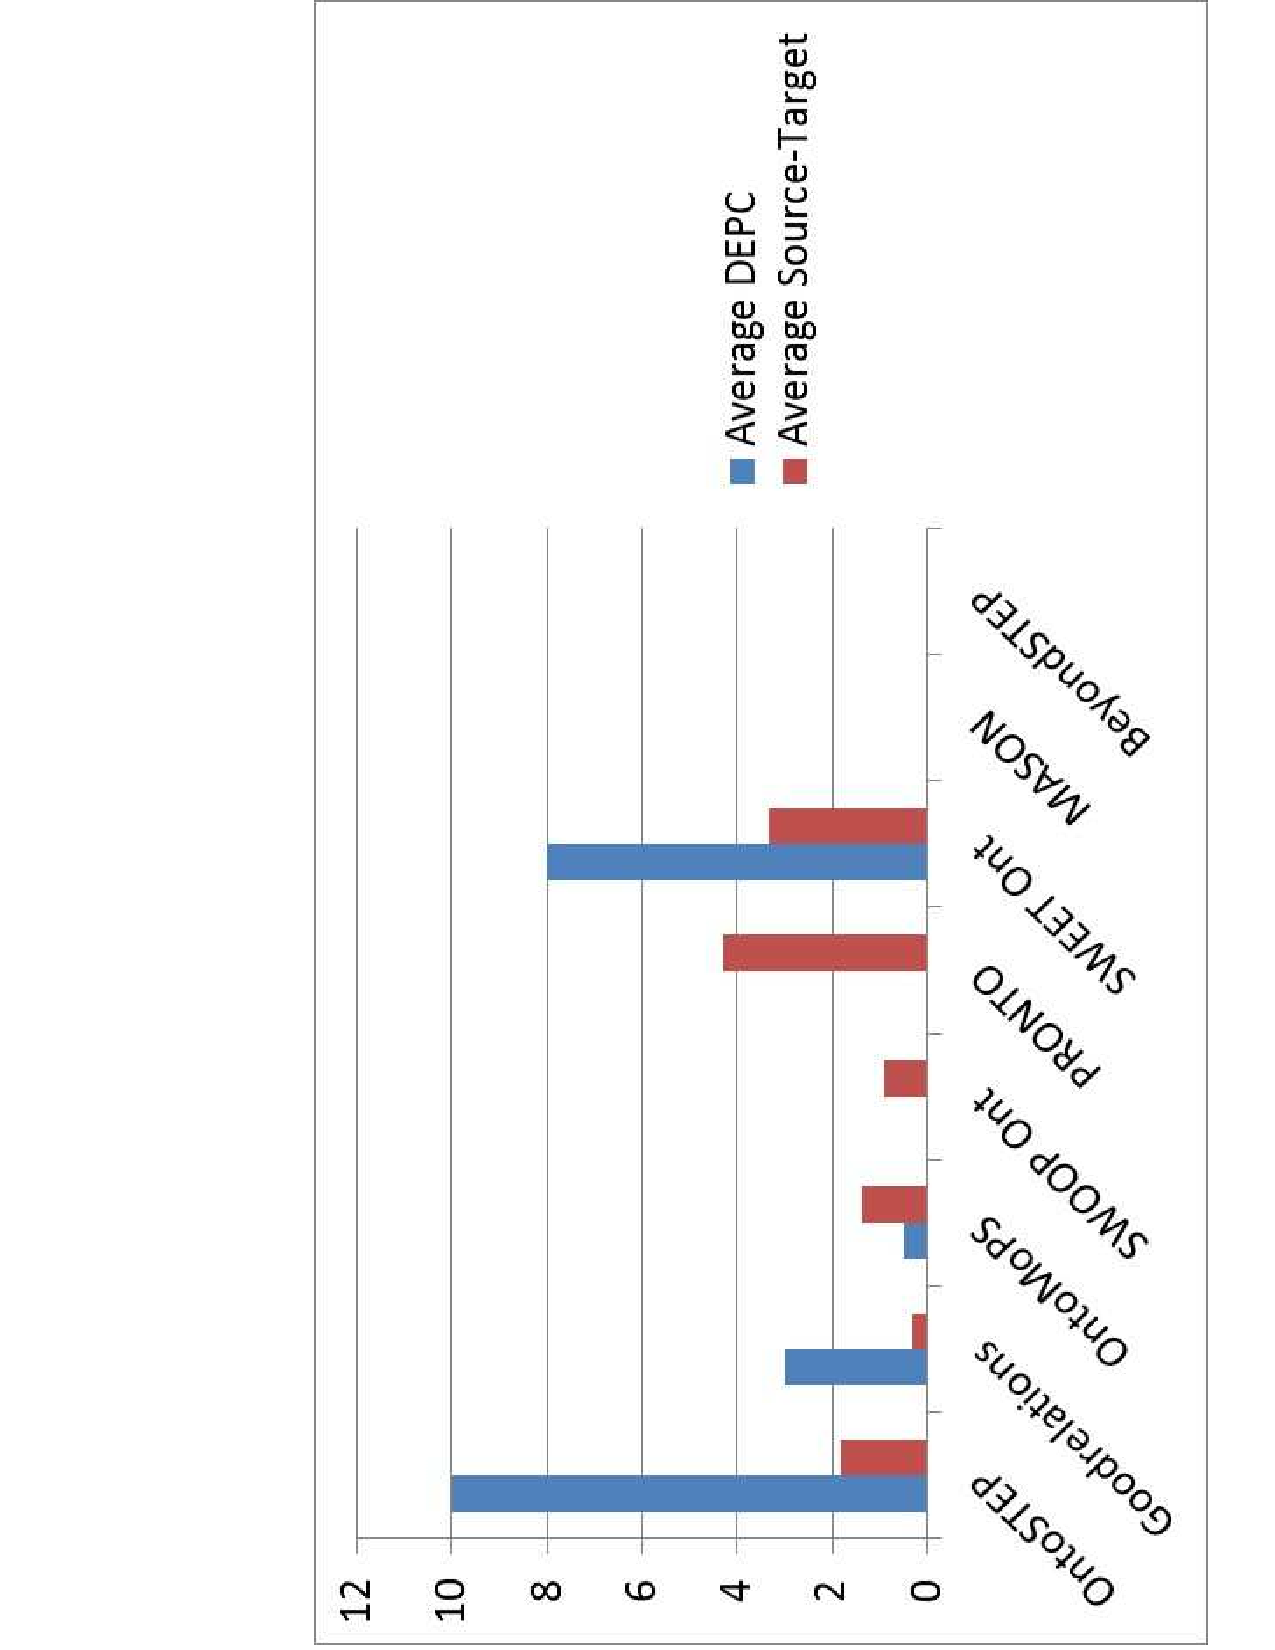
\includegraphics[scale=0.5, angle=-90]{figure-chapterIV/fig4-13.pdf}\\
		\caption{Relative Upper Relationship among Ontologies}
		\label{figure4-13}
	\end{center}
\end{figure}



With the definition of the previous metrics, we calculated the results for the adopted ontologies, and  display the results in Fig. \ref{figure4-13}. As we stated in the previous paragraphs, when the concept of deployment measurement  was introduced, this evaluation is intended to determine: first how an upper ontology is compared to other pairs of ontologies that have mappings among them and, second, the interoperability level  that could be provided by this ontology in a hypothetical network of systems where the other ontologies are implemented. For authors like \cite{borgo_role_2004}, this interoperability is granted by means of shared ontologies, but while they provide a subjective method for alignment of \gls{ulo}´s with manufacturing ontologies, and other authors like \cite{lemaignan_mason:_2006} declare their manufacturing ontologies as \gls{ulo}´s without providing enough support for such a statement, we consider that more objective metrics are required. In this vein the figure depicted above breaks down how the results were obtained applying the metrics to the network of ontologies shown in Fig. \ref{figure4-10}. That is, the upper relationship between ontology and its respective mapping environment. Unlike the previous  views provided in Fig. \ref{figure4-9} and Fig. \ref{figure4-10}, with the results depicted in Fig. \ref{figure4-13}, we have a criterion to determine how upper an ontology is compared to others in a network. 


Fig. \ref{figure4-10} introduced above is interpreted as follows: Every ontology evaluation yields two columns. The left column corresponds to the average of  deployment of concepts among the ontology evaluated as an upper one, and the right column corresponds to the  average of mapped   concepts in the source and the target ontology. To consider one of the evaluated ontologies as relatively upper in comparison to the others within the network under study, the two following assumptions are made:

\begin{itemize}
	\item [a] The column on the left should be smaller than the column on the right for the ontology under evaluation. When this occurs, it means that the deployment of mapped concepts in source and target ontologies is larger than the deployment in the upper ontology.
	
	\item [b] The column on the left is greater than 2. This value for the source and target indicates that for each mapping concept at least two new concepts are linked to it by arcs. This means that, as in the previous points, the mapped concept has been deployed in the source and target ontologies, and that it is not a mapping with a leaf node.
	
\end{itemize}

According to the criterion indicated above, and considering the results depicted in Fig. \ref{figure4-13}, we can mention that in the manufacturing network of ontologies shown in Fig. \ref{figure4-10} there is a lack of any single ontology that could be considered to occupy a relatively upper level in the network. In other words, according to our metrics, none of the manufacturing ontologies evaluated would serve as an interoperability artifact among other ontologies. 

The relevance of this discussion on the presence of \gls{ulo}´s in the network of ontologies presented in Fig. \ref{figure4-10} lies on one hand in the fact that some of the ontologies presented used in this evaluation have been declared as \gls{ulo}´s by their proponents without supporting   their statements in a detailed analysis of previously existing ontologies in the domain. \gls{mason} and \gls{swop} are some of these \gls{ulo}s. On the other hand, although the concept of \gls{ulo} is clearly defined from the philosophical point of view and many \gls{ulo}´s are clearly identified, the category of ontologies according to the hierarchy indicated in \cite{gomez_perez1}  is still subjective. This issue may cause interoperability misinterpretations when using an ontology in a hierarchy higher than where it should be according to its \textit{ontological contribution} to the given target domain, manufacturing in our case. Consequently, with this partial result of our research, in Fig. \ref{figure4-13} we highlight the necessity of evaluation of ontologies in a given network of ontologies  prior to declaring them as \gls{ulo}s. If we declared ontology to be upper level for a given domain, to our knowledge it means it can be used to enable interoperability between systems that use lower level ontologies. This “level” of the ontology is not related to quality, but with reusability. This means the more, \textit{upper the ontology} the more reusable it is, because it is more general, however the upper is the ontology the less usable it is, which is a disadvantage. Therefore, Ontological engineers shall be able to manage such a categorization. 

From our point of view, what some authors have tried to express when declaring their ontologies as \gls{ulo}´s, is that they assume their ontologies have a higher level of reusability than the other ontologies they compared in their studies. Such a feature would make their ontologies more reusable, but according to our evaluation it is not simple to highlight one of the evaluated ontologies for permitting interoperability among the others. 

Because it was not possible to find the ontology category of Upper Level in the evaluated network. In the following subsection, we will proceed to describe the next steps of our methodology in order to determine whether or not it is possible to establish other kinds of relations between those manufacturing ontologies. 

\subsection{Hyper Modules Extraction}\label{subsection4.2.5}

As discussed in previous Subsections, modularity can be pursued as an alternative to the \gls{ulo} approach, intended to enable maintenance, publication, validation and processing of ontologies \cite{daquin_modular_2009}. Two main modularity approaches have been distinguished from each other in the literature, the former corresponds to the division of a large ontology into modules, thus rendering such an ontology to be more manageable, and the latter corresponds to the generation of small modules from links between some collections of ontologies in an storage.  Defining so-called ‘hyperlinks’ between ontologies is intended to enable the interconnection of    related ontologies, but without merging the logical content of those ontologies. 

In addition to mappings between concepts that are considered equivalent, which is the foundation of hyperotological networks, we argue that the identification and consideration of subsumption relations   between equivalent concepts in this Hyperontology will allow us to identify \textit{hypermodules}. Onto\textit{Smart} provides algorithms 1\footnote{shorturl.at/aknIM} and 2\footnote{shorturl.at/htKTW} to identify such modules. 

 

\begin{table}[tp]%

\caption{List of Monomodules}
\label{table4.6}\centering
\begin{tabular}{ p{4cm}}\toprule
	
	\textbf{Monomodules} \\\toprule
	Event\\\toprule
	Material\\\toprule
	Set\\\toprule
	Organization\\\toprule
	Person\\\toprule
	
\end{tabular}

\end{table}


As we indicated above, with the implementation of our algorithm in the network of ontologies presented in Fig. \ref{figure4-10} it was also possible to find a group of six hyper-modules of multi-module type. Every multi-module, contains several concepts subsumed by a root concept which in turn is connected to another concept in another ontology through mapping. These modules were named \texttt{Unit, Product, Process, Features, Resources} and \texttt{Geometry}. Regarding the specific concepts, it is necessary to remember the list of concepts mentioned in Subsection \ref{subsection4.2.4} proposed by \cite{martin_design_2003} and \cite{lastra_ontologies_2009} as significant for the manufacturing domain. Those terms are \texttt{Product, Process, Resource} and \texttt{Equipment}. Moreover, we are including the root concepts \texttt{Unit, Features, Geometry} and the concepts \texttt{event, material, set, organization} and \texttt{person} (\texttt{mono-modules}). With this information we proceeded to present every resulting hyper module of multi-module type, at first for every-module evaluating graphics is presented, and then an ontological view of the module is shown, this view was obtain after editing the hierarchical view of the hyper module in an ontology editor, Protégé for this case. After describing every hyper module, they will be included in a single view that integrates the hyper modules of the Hyperontology with the network of ontologies.

\subsubsection{Hyper module of Unit}\label{subsubsection4.2.5.1}

In Subsection \ref{subsection4.2.4} we introduced Table \ref{table4.5} to present the most frequent terms found in the network of ontologies shown in Fig. \ref{figure4-10}. With the application of our proposed algorithm, the concept \texttt{Unit} appears again as a part of a hyper module of multi module type. This concept is integrated with the concepts \texttt{BaseUnit}, \texttt{Mega}, \texttt{micro}, \texttt{meter} and \texttt{degree Celsius}. It is necessary to mention the relevance of these terms for Science and Engineering,   given that metrology, as the science of measurement, takes part in those fields. Nevertheless, besides the importance of the term \texttt{Unit} for manufacturing, it  does not appear in every ontology of the network; moreover the other terms that form part of this hyper module appears in only 2 of those ontologies.   

In Fig. \ref{figure4-16} we show the results obtained calculating the values of \gls{bs} and \gls{ds}  of the concept \texttt{Unit}   and some of its subsumed terms among ontologies included in network  shown in Fig. \ref{figure4-10}. There, the concepts present in this multi-module are evaluated in two steps: first an evaluation of the ontologies that contain the concept \texttt{Unit} and, second, around every term subsumed by \texttt{Unit}. Most of the terms presented there have a \gls{bs} of 0.4 and a \gls{ds} of 0.26. This result means that, although the \gls{bs} is closer to 50\%, when measuring the domain under study, the average \gls{ds} indicates a weakness more than a strength on the terms related to \texttt{Unit}. Going into details, the term \texttt{Unit} is presented in 5 of 8 ontologies of the network, while the other terms are present only in 2 of 8. 


\begin{figure}
\begin{center}
	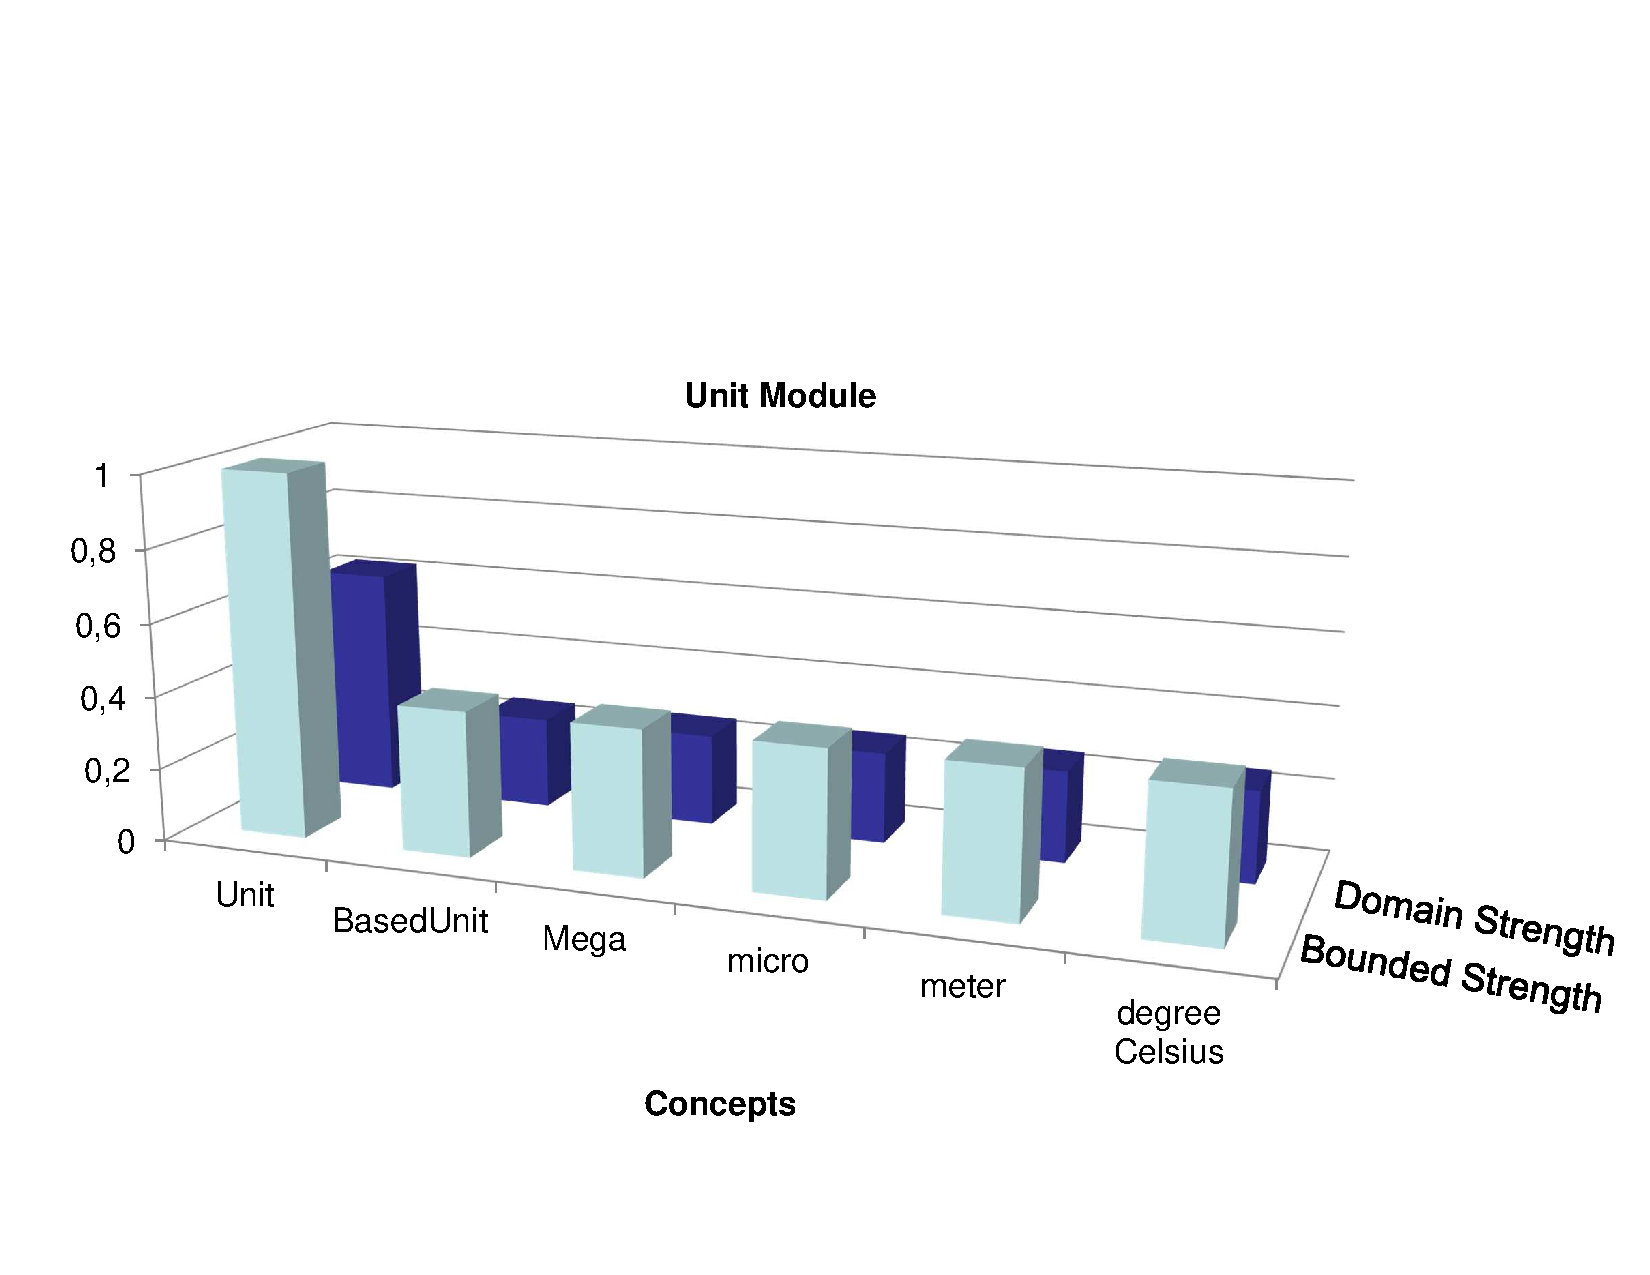
\includegraphics[scale=0.5]{figure-chapterIV/fig4-16.pdf}\\
	\caption{Strength of Concepts Bounded by Unit}
	\label{figure4-16}
\end{center}
\end{figure}

\begin{figure}
\begin{center}
	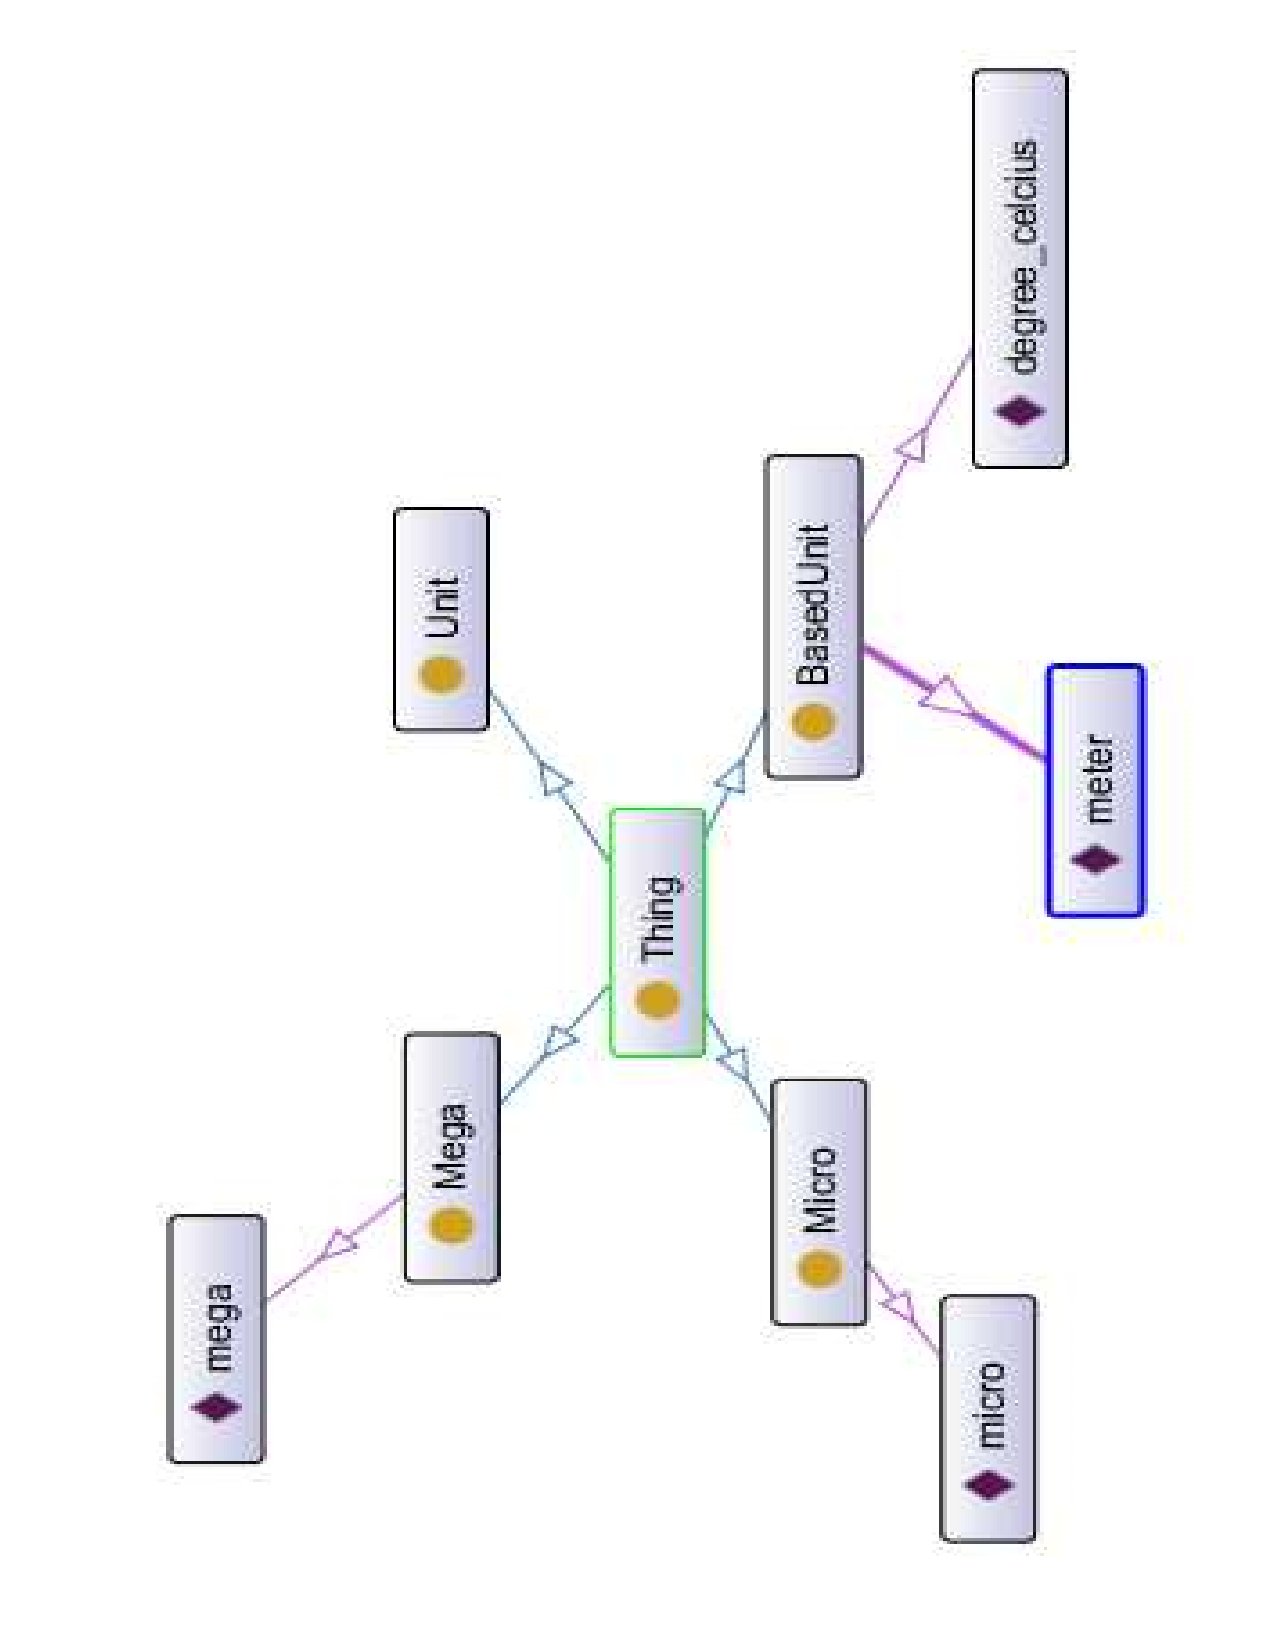
\includegraphics[scale=0.5, angle =270]{figure-chapterIV/fig4-17.pdf}\\
	\caption{Partial Hyperontology for the term \texttt{Unit} graphed with Protégé}
	\label{figure4-17}
\end{center}
\end{figure}


Fig. \ref{figure4-17} shows the concepts and instances that appear mentioned in Fig. \ref{figure4-16}. This set of concepts was obtained as a partial result of executing the \texttt{compute\_hypermodule} routine which is part of our algorithm. This figure shows the result as an ontology. 

\subsubsection{Hyper module of Product}\label{subsubsection4.2.5.2}

Similarly, and following the procedure described above, the Hyper module \texttt{Product} was obtained. This hyper module is integrated   by the terms \texttt{Product, Part} and \texttt{Assembly}. It is worth noting the relevance of these terms in Semantic Manufacturing because,   on the one hand the Product can be considered the center of this conceptualization, and products many times are integrated by some type of parts, generating an assembly. On the other hand the presence of the concepts \texttt{Part} and \texttt{Assembly} in this hyper module indicates the existence of a relation that comprises the product, and this type of relation is known as part-hood relations. Later, as part of our methodology, when Axiomatization and Heterogeneity activities take place, the part-hood relations issued by \gls{owl}, will be taken up and discussed. Below we present the analysis related to this hyper module. 


\begin{figure}
\begin{center}
	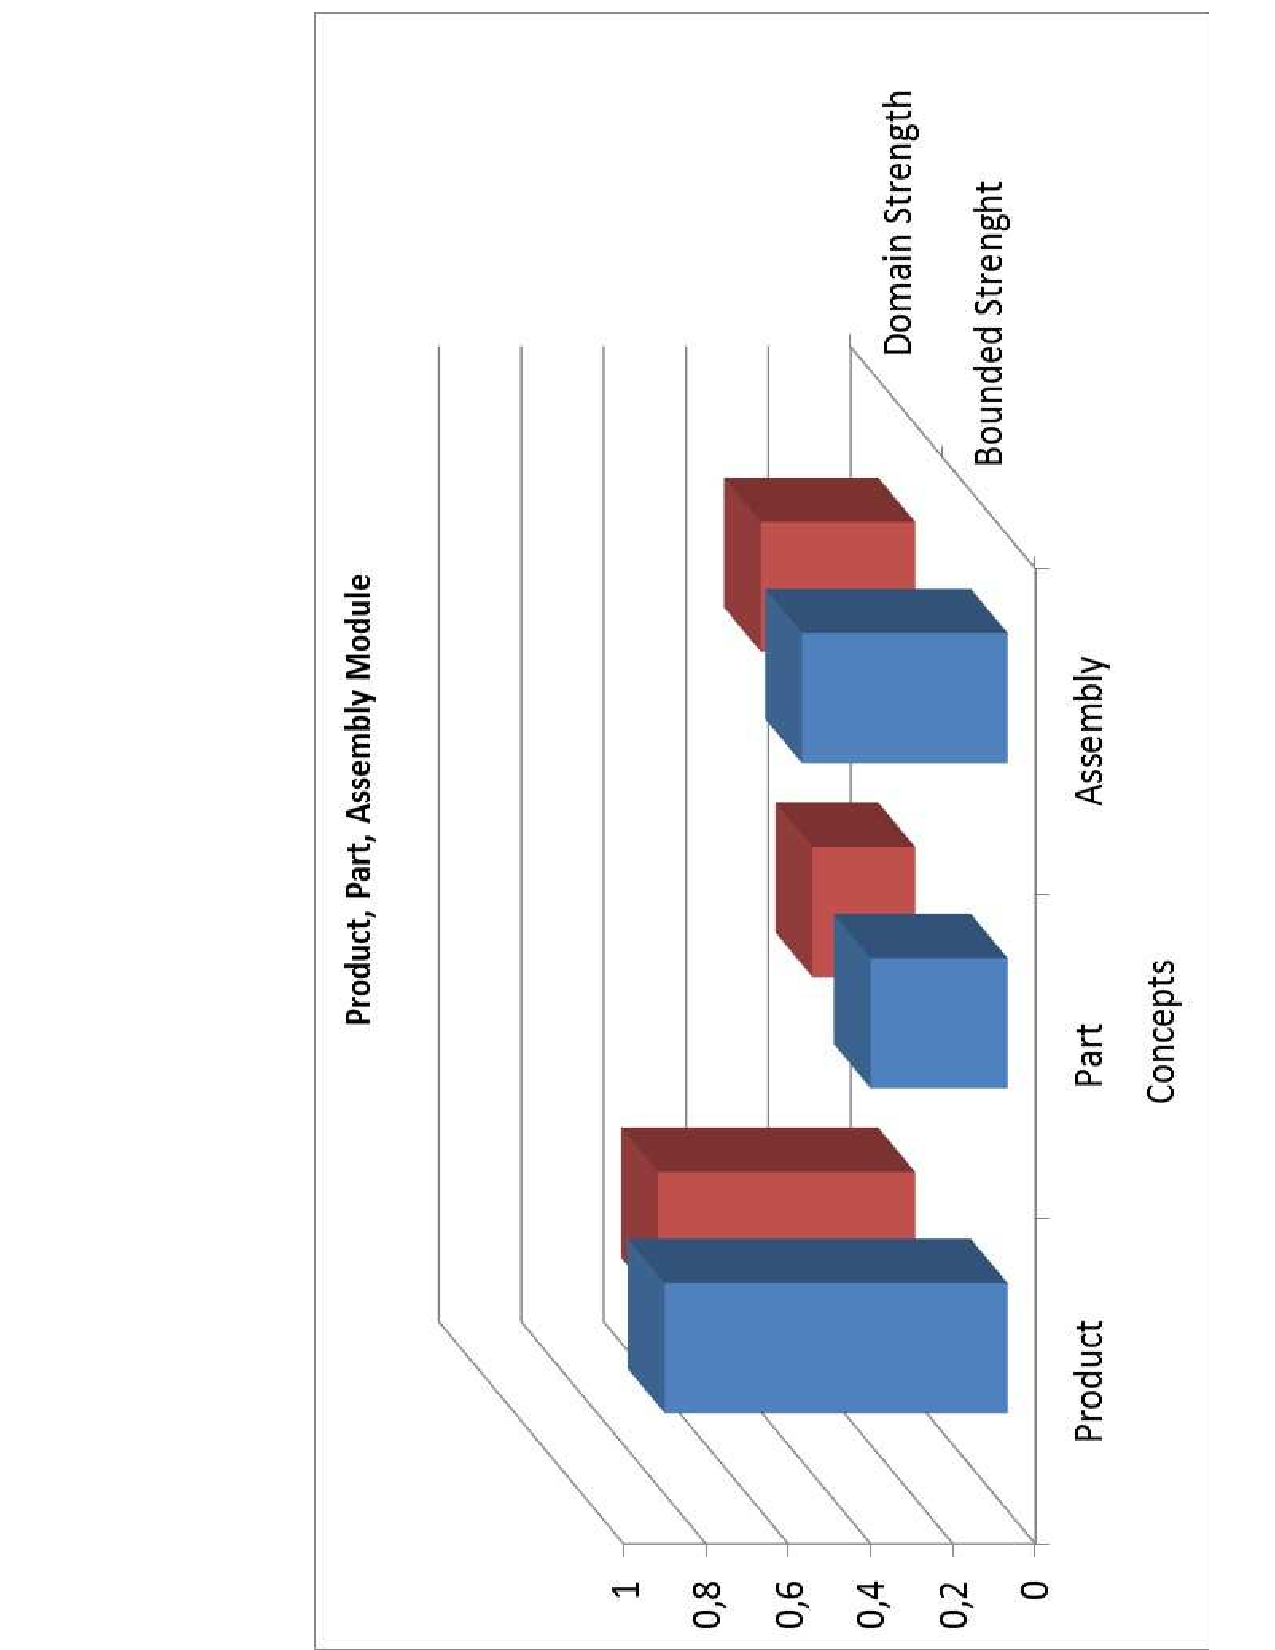
\includegraphics[scale=0.5, angle=-90]{figure-chapterIV/fig4-18.pdf}\\
	\caption{Product Hyper Module}
	\label{figure4-18}
\end{center}
\end{figure}

\begin{figure}
\begin{center}
	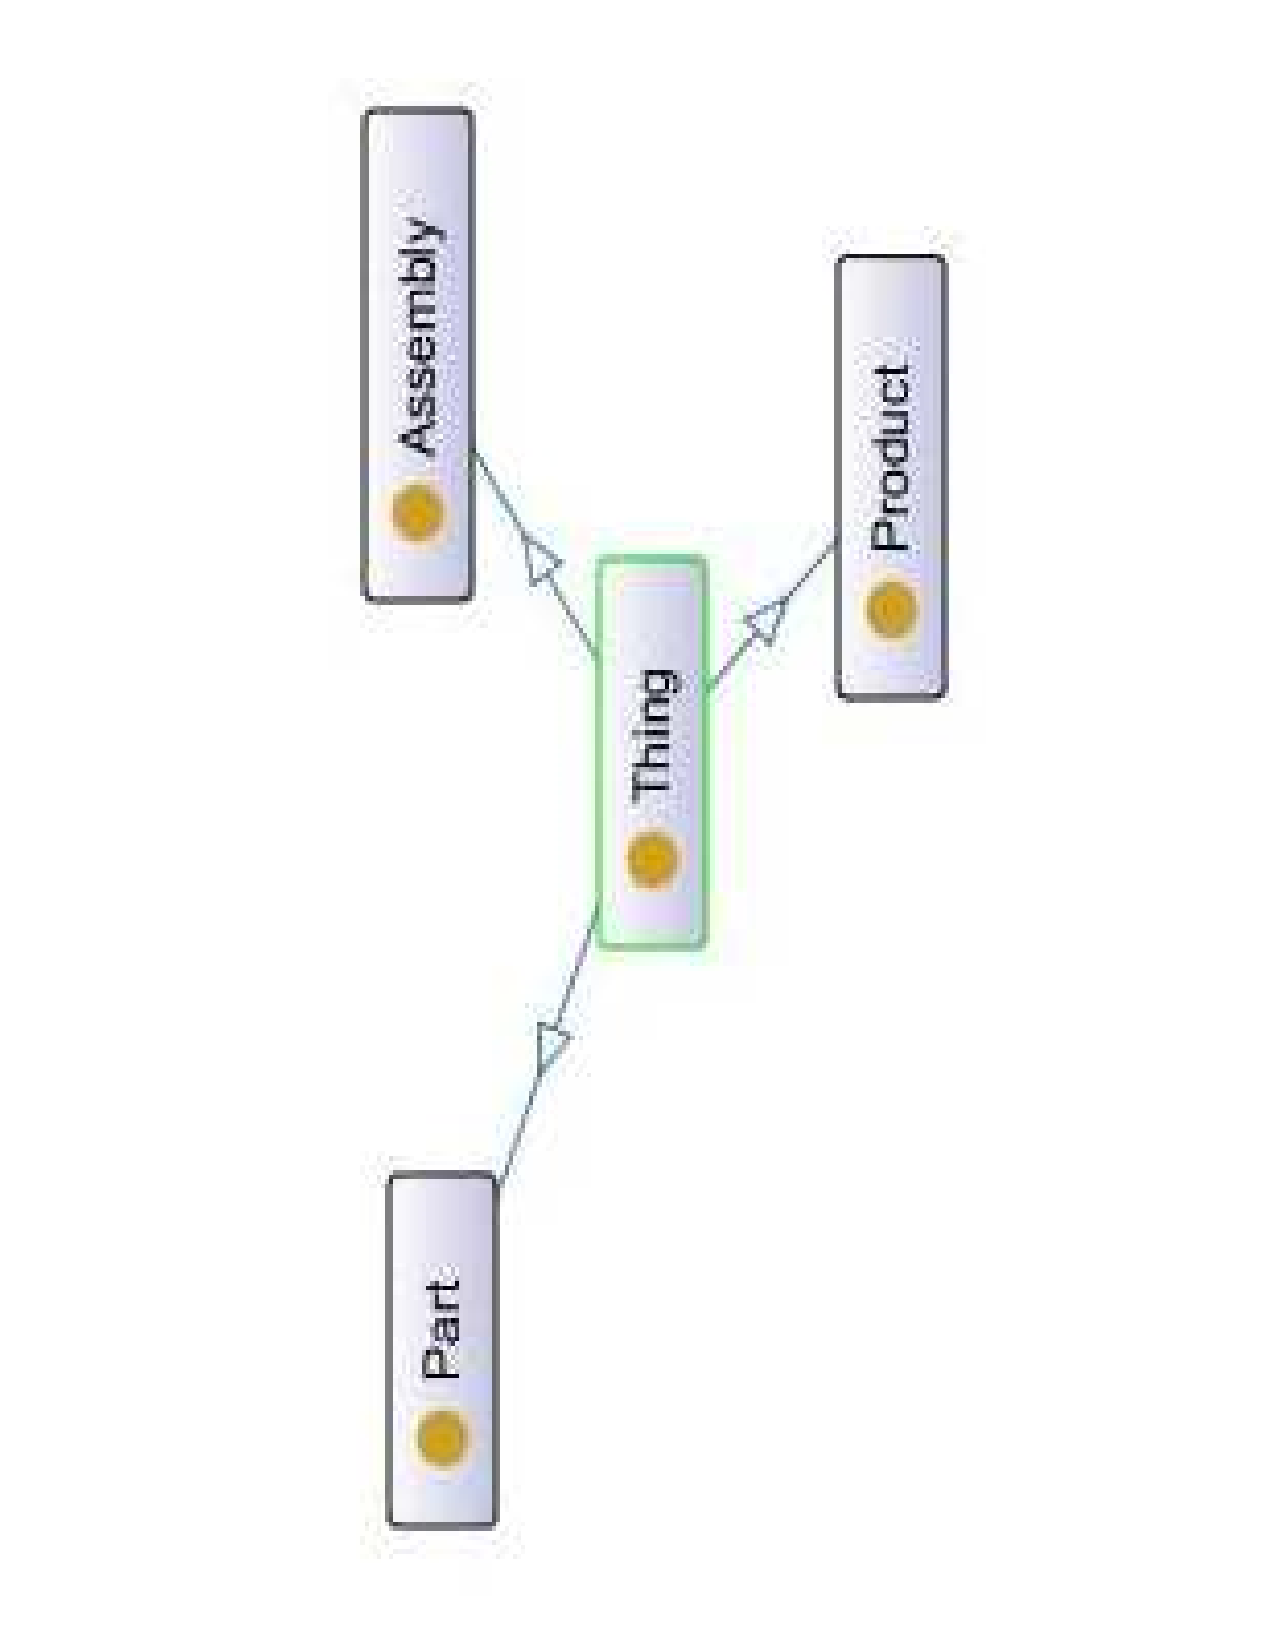
\includegraphics[scale=0.5, angle=270]{figure-chapterIV/fig4-19}\\
	\vspace{-20mm}
	\caption{Members of the Hypermodule Product}
	\label{figure4-19}
\end{center}
\end{figure}


Fig. \ref{figure4-18} shows the results of the statistical analysis we performed, which is the term \texttt{Product} has a \gls{bs} of 0.83, followed by \texttt{Assembly} with a \gls{bs} of 0.5; and the term \texttt{Part} with a \gls{bs} of 0.33 Moreover \texttt{Product} has a \gls{ds} of 0.625 followed by \texttt{Assembly} and \texttt{Part} with a \gls{ds} of 0.375 and 0.25 respectively. In the case of the term \texttt{Part}, and following a criterion similar to the one used for the hyper module \texttt{Unit}, we can state that there is a weakness in it, which means there is a low likelihood of achieving interoperability through it.  After analyzing  this hyper module according to the proposed \gls{bs} and \gls{ds} metrics, we proceed to represent it as an ontology in Fig. \ref{figure4-19}. This figure corresponds to a simplified view given that the corresponding ontologies, and other hyper-modules have to be integrated in a complete view, present in the hyper ontology as integrated by hyper modules in an ontologies network. 


\subsubsection{Hyper-module of the Process}\label{subsubsection4.2.5.3}

Following the statistical   analysis of results, Fig. \ref{figure4-20} introduced the hyper module of \texttt{Process}. \texttt{Process} and \texttt{Operation} are meaningful concepts for the manufacturing domain. In this vein, the concept \texttt{Process} has been mostly adopted to define ontologies related to this terminology. Nevertheless, from the graphic it can be concluded that in this network the concept \texttt{Operation} is found with more strength   (\gls{bs}: 0.6) than the concept \texttt{Process} (\gls{bs}: 0.4). Other terms found in this Hypermodule were \texttt{Change}, related to \texttt{Process} and \texttt{Operation}, and the terms \texttt{Cutting, Drilling, Milling} and \texttt{Addition}. 

The last four terms mentioned above are closely related (\texttt{Cutting}, \texttt{Drilling}, \texttt{Milling} and \texttt{Addition}), given that   the three terms correspond to a manufacturing application domain named machining, and all of them belong to \gls{mason}. We go into details of these results because the authors of \gls{mason} declared it is an Upper Level Ontology. These concepts have a low \gls{bs} and \gls{ds} (0.2 and 0.125 for each respectively) which makes them highly usable, but less reusable because of their specificity. This result is not necessarily related to quality, because the effectivity of this ontology will depend more on the skills of the ontologist than the ontology itself. But, the resulting values of \gls{bs} and \gls{ds} of those \gls{mason} concepts serves  to categorize \gls{mason} as an Application Domain Ontology. This is not an isolated result. In previous Section we  mentioned the research of other authors who have made similar remarks about their work, but with the implemented metrics,  procedures followed, and results obtained, the classification made by these authors  on  ontologies as \gls{ulo}´s can be questioned. 


\begin{figure}
\begin{center}
	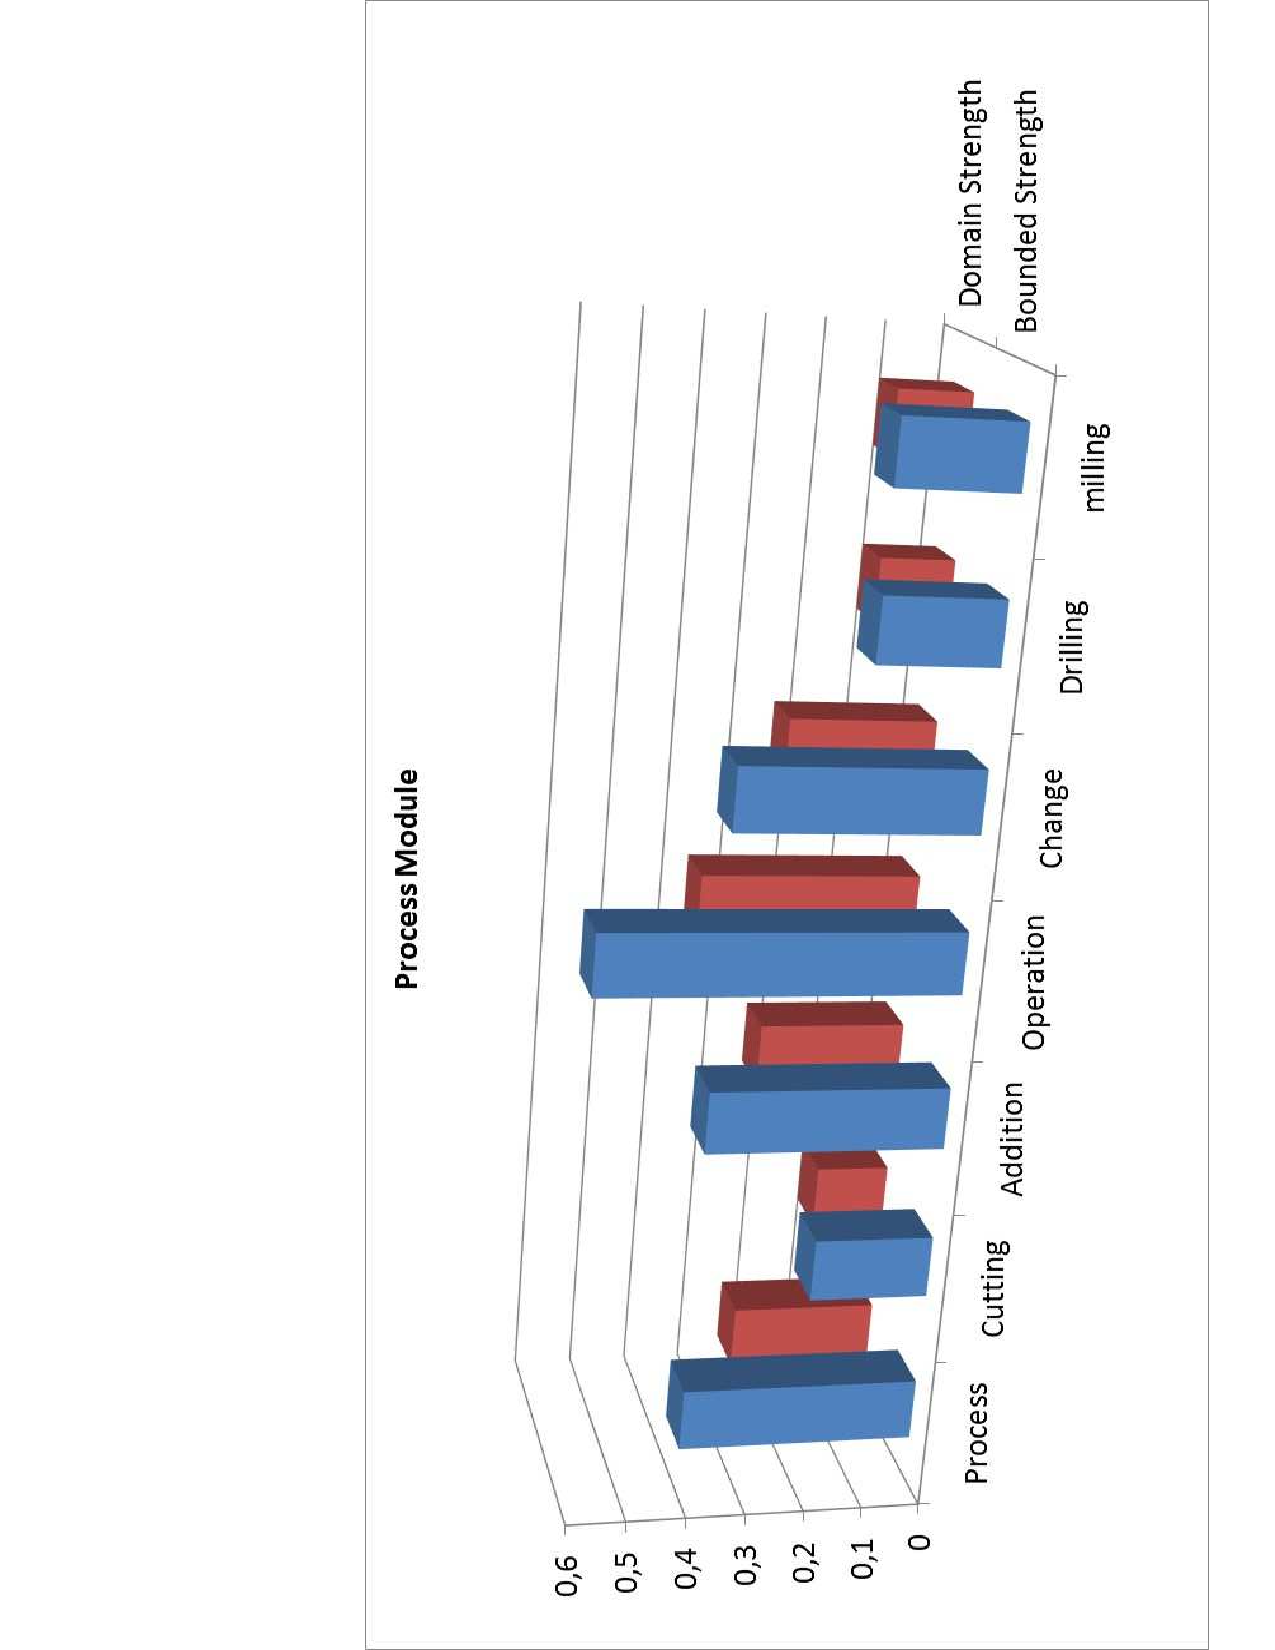
\includegraphics[scale=0.5, angle=-90]{figure-chapterIV/fig4-20}\\
	\caption{Hyper Module Process}
	\label{figure4-20}
\end{center}
\end{figure}

\begin{figure}
\begin{center}
	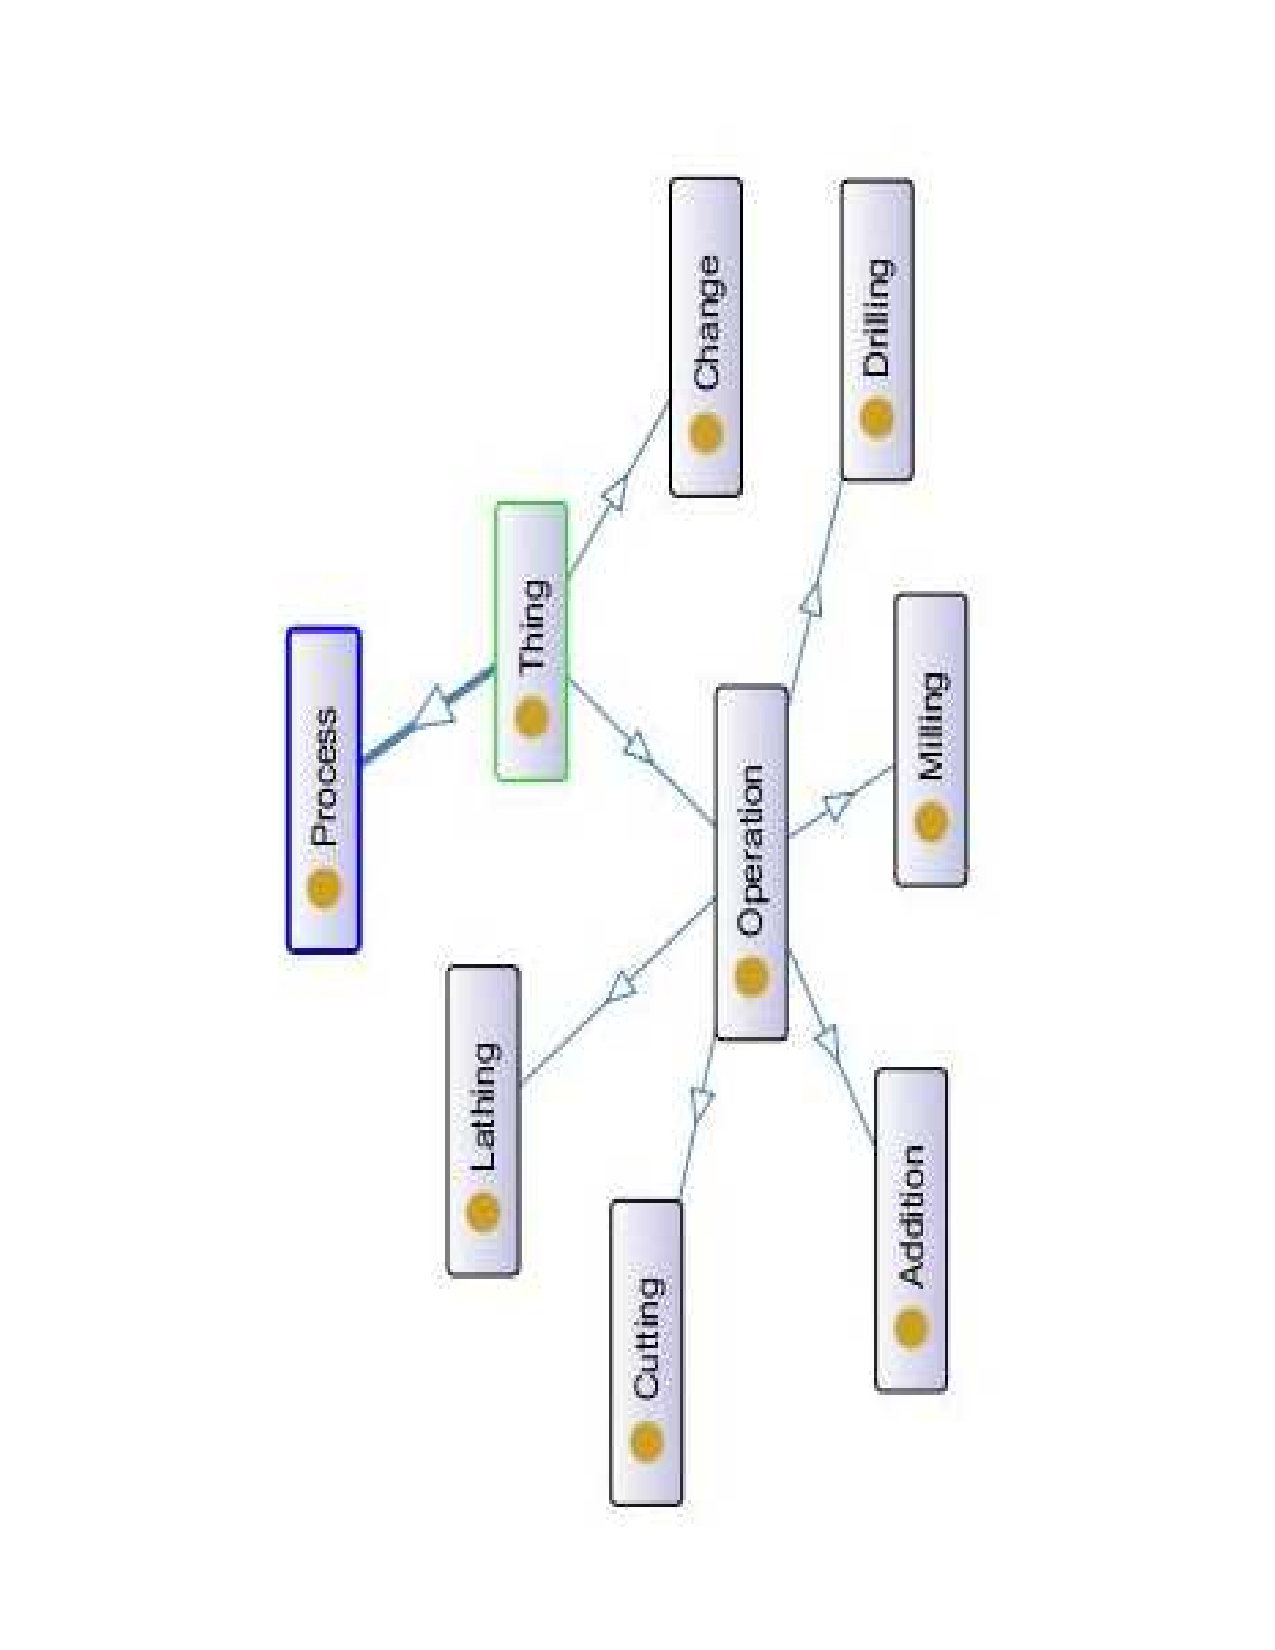
\includegraphics[scale=0.5, angle=270]{figure-chapterIV/fig4-21}\\
	\vspace{-40mm}
	\caption{Hyperontology of Process}
	
	\label{figure4-21}
\end{center}
\end{figure}

In Fig. \ref{figure4-21} we introduce an ontological view of the Hyperontology of the \texttt{Process} as resulting from Fig. \ref{figure4-21}. The concept \texttt{Operation} was used as root concept for specific operations due to its higher \gls{ds} (0.375), while \texttt{Process} and \texttt{Change} remained  at the same \texttt{Operation} level. \textbf{meaning}

\subsubsection{Hyper module of Features}\label{subsubsection4.2.5.4}


Continuing with our Hypermodule extraction, we processed a hyper module containing some features commonly found in mechanization processes. We named this hyper module of features. Some of the concepts contained by this module are \texttt{Circular\_Pattern}, \texttt{Threat}, \texttt{Slot}, \texttt{Pocket}, and \texttt{Chamfer}. Most of the terms were found in \gls{mason} and Onto STEP, which will allow information exchange among both ontologies. It is necessary to highlight that the features mentioned below are common in mechanization processes, but they are not the only ones and they were also not found in the other 6 ontologies. For instance, \gls{pronto} was proposed to represent products and their features, however no hyper-mapping was found in the network, because   they referred to different Application Domains: \gls{mason} corresponds to machining processes, and \gls{pronto} to breaking up or separating processes.


\begin{figure}
\begin{center}
	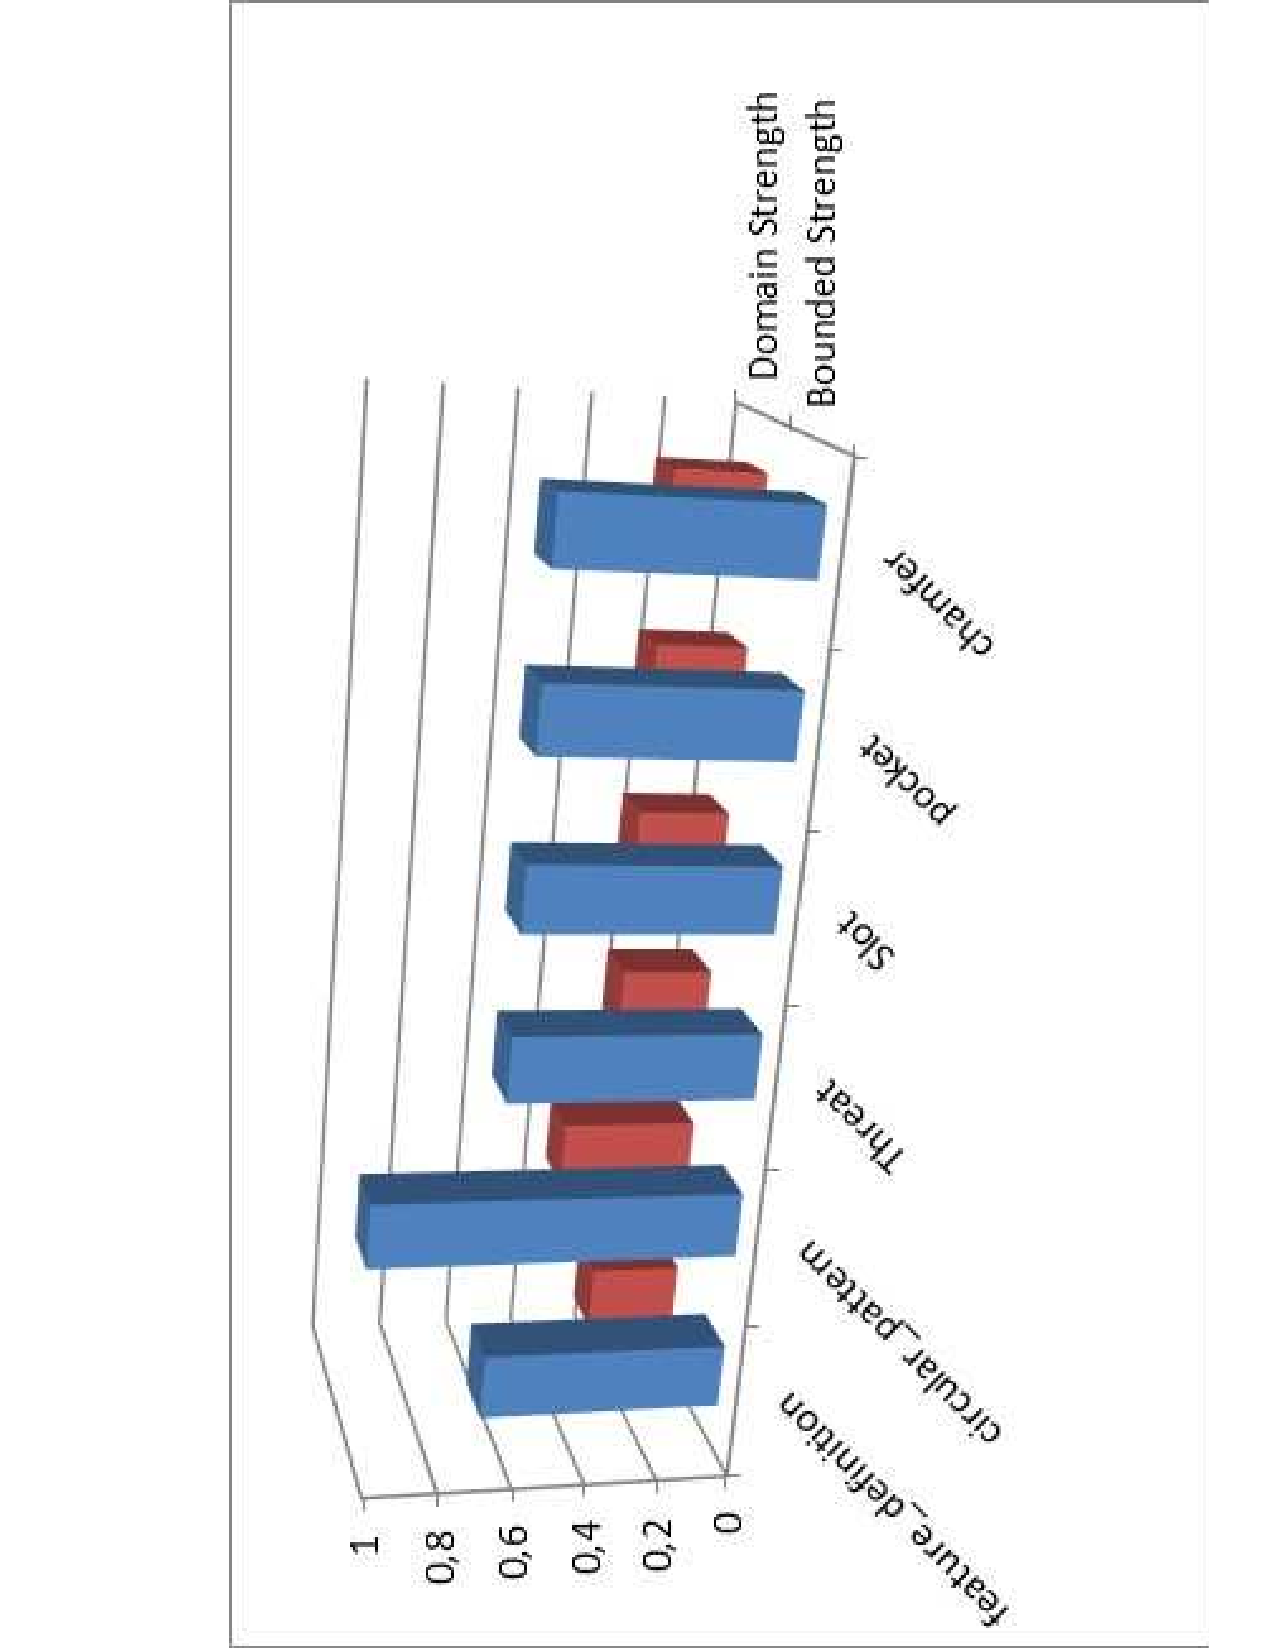
\includegraphics[scale=0.5, angle=-90]{figure-chapterIV/fig4-22.pdf}\\
	\caption{Hypermodule of Features}
	\label{figure4-22}
\end{center}
\end{figure}

Fig. \ref{figure4-23} shows the Hyperontology of Features, where concept \texttt{Features} is the  root concept in this ontology. These Features mostly apply to mechanization procedures. 


\begin{figure}
\begin{center}
	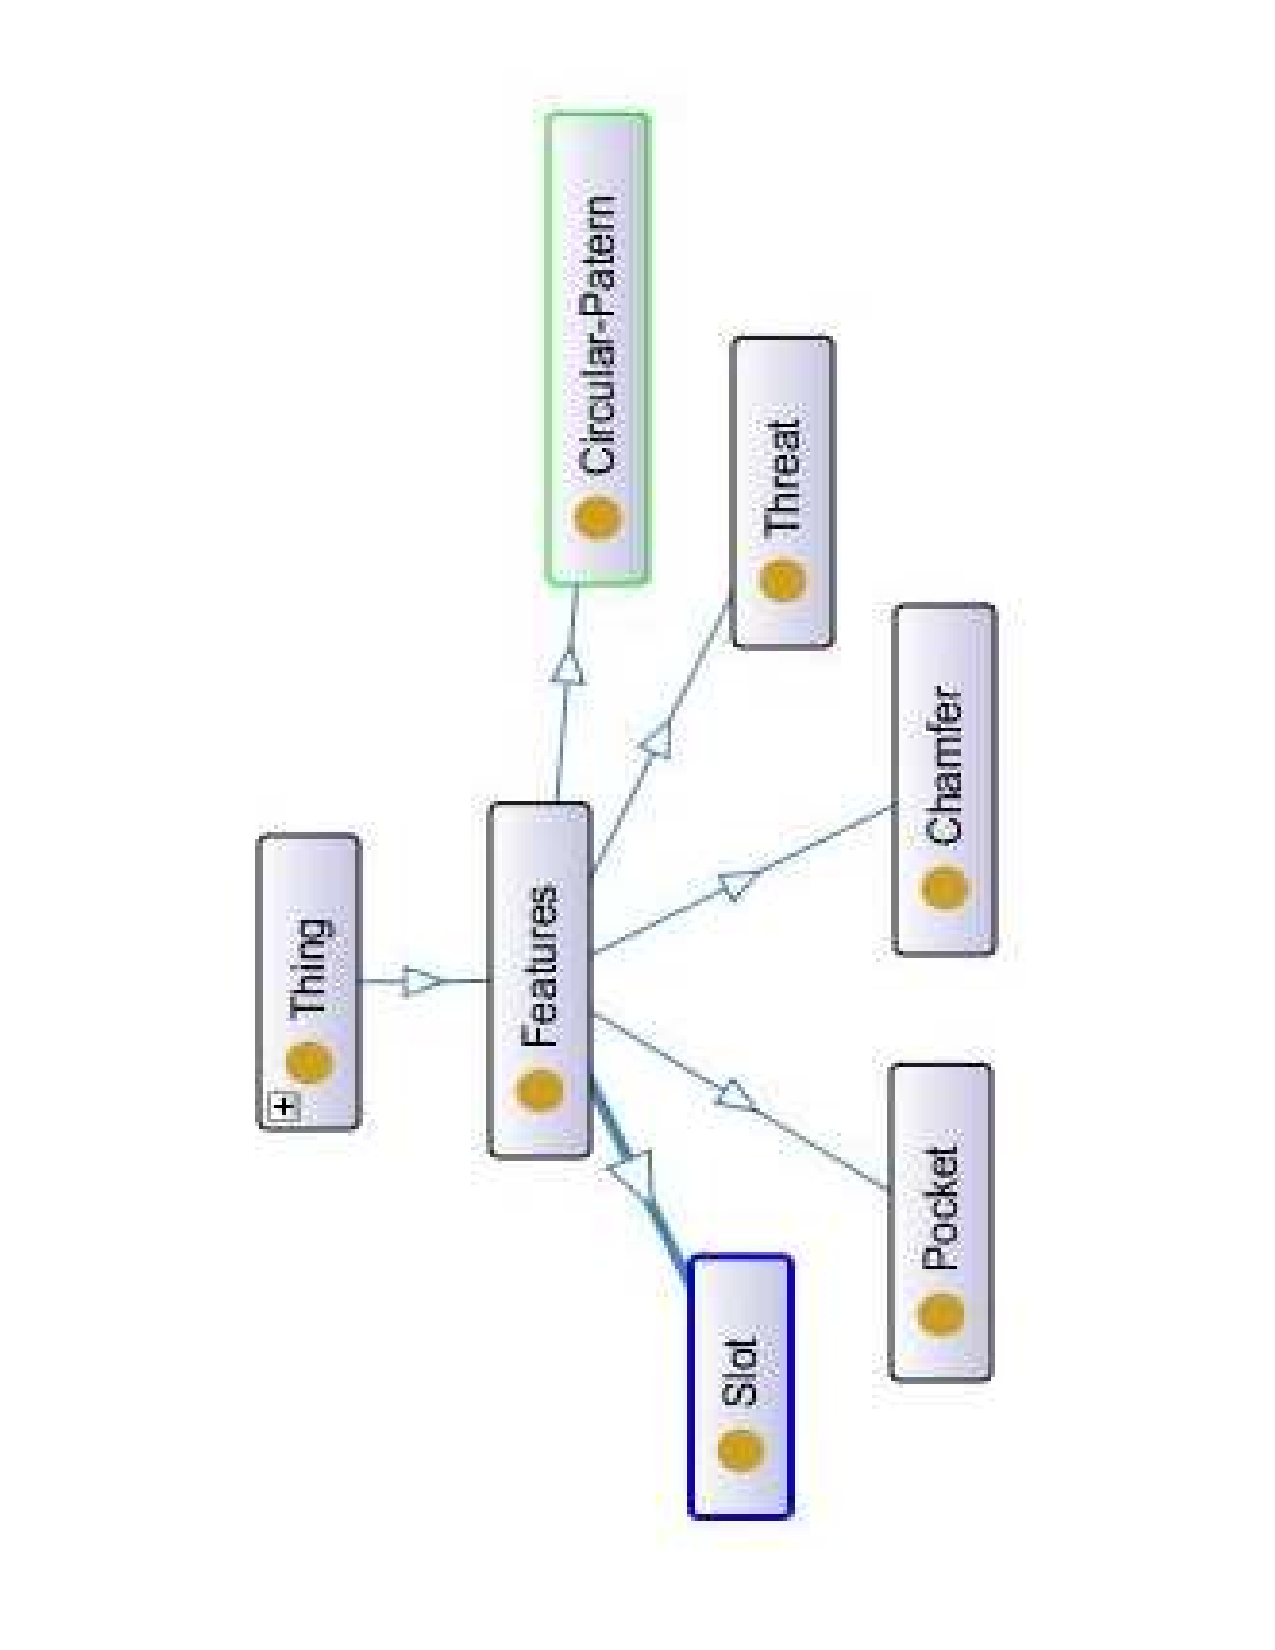
\includegraphics[scale=0.5, angle=270]{figure-chapterIV/fig4-23}\\
	\caption{Hyperontology Features}
	\label{figure4-23}
\end{center}
\end{figure}

Continuing with the description of the hyper modules obtained by the execution of the proposed algorithm, we obtained \texttt{Resource, Machine, Tool, Lathe} and \texttt{Drill} concepts. All these concepts were  found in the \gls{mason} and OntoMoPS ontologies, while in OntoSTEP only 2 of them were found. 

If we return to the results previously obtained during the evaluation of the Hyper module of Features, we found that the features and the resources to get the features manufactured on the raw material are present in the \gls{mason} ontology as well. For instance, with a Lathe we can make circular patterns. This is a commonality that until now has only appeared in this case. Where \gls{mason} appears with common concepts that relates two pairs of ontologies: a first pair OntoStep-\gls{mason} where the concept \texttt{Feature} is developed, and a second pair \gls{mason}-OntoMoPS where the concept \texttt{Resource} is developed. Some of the resources mentioned in the latter pair are required as machinery for manufacturing the Feature mentioned in the former pair. 

In this vein, Fig. \ref{figure4-24} contains the result of applying the \gls{bs} and \gls{ds} parameters to the network where these \texttt{Resource} and \texttt{Drill} concepts have a \gls{bs} of 1, while the others have a \gls{bs} of 0.66. Besides having the same \gls{bs} value, \texttt{Resource} is more general than \texttt{Drill}, where \texttt{Drill} is a type of machining. The resulting ontology is shown in Fig. \ref{figure4-25}.


\begin{figure}
\begin{center}
	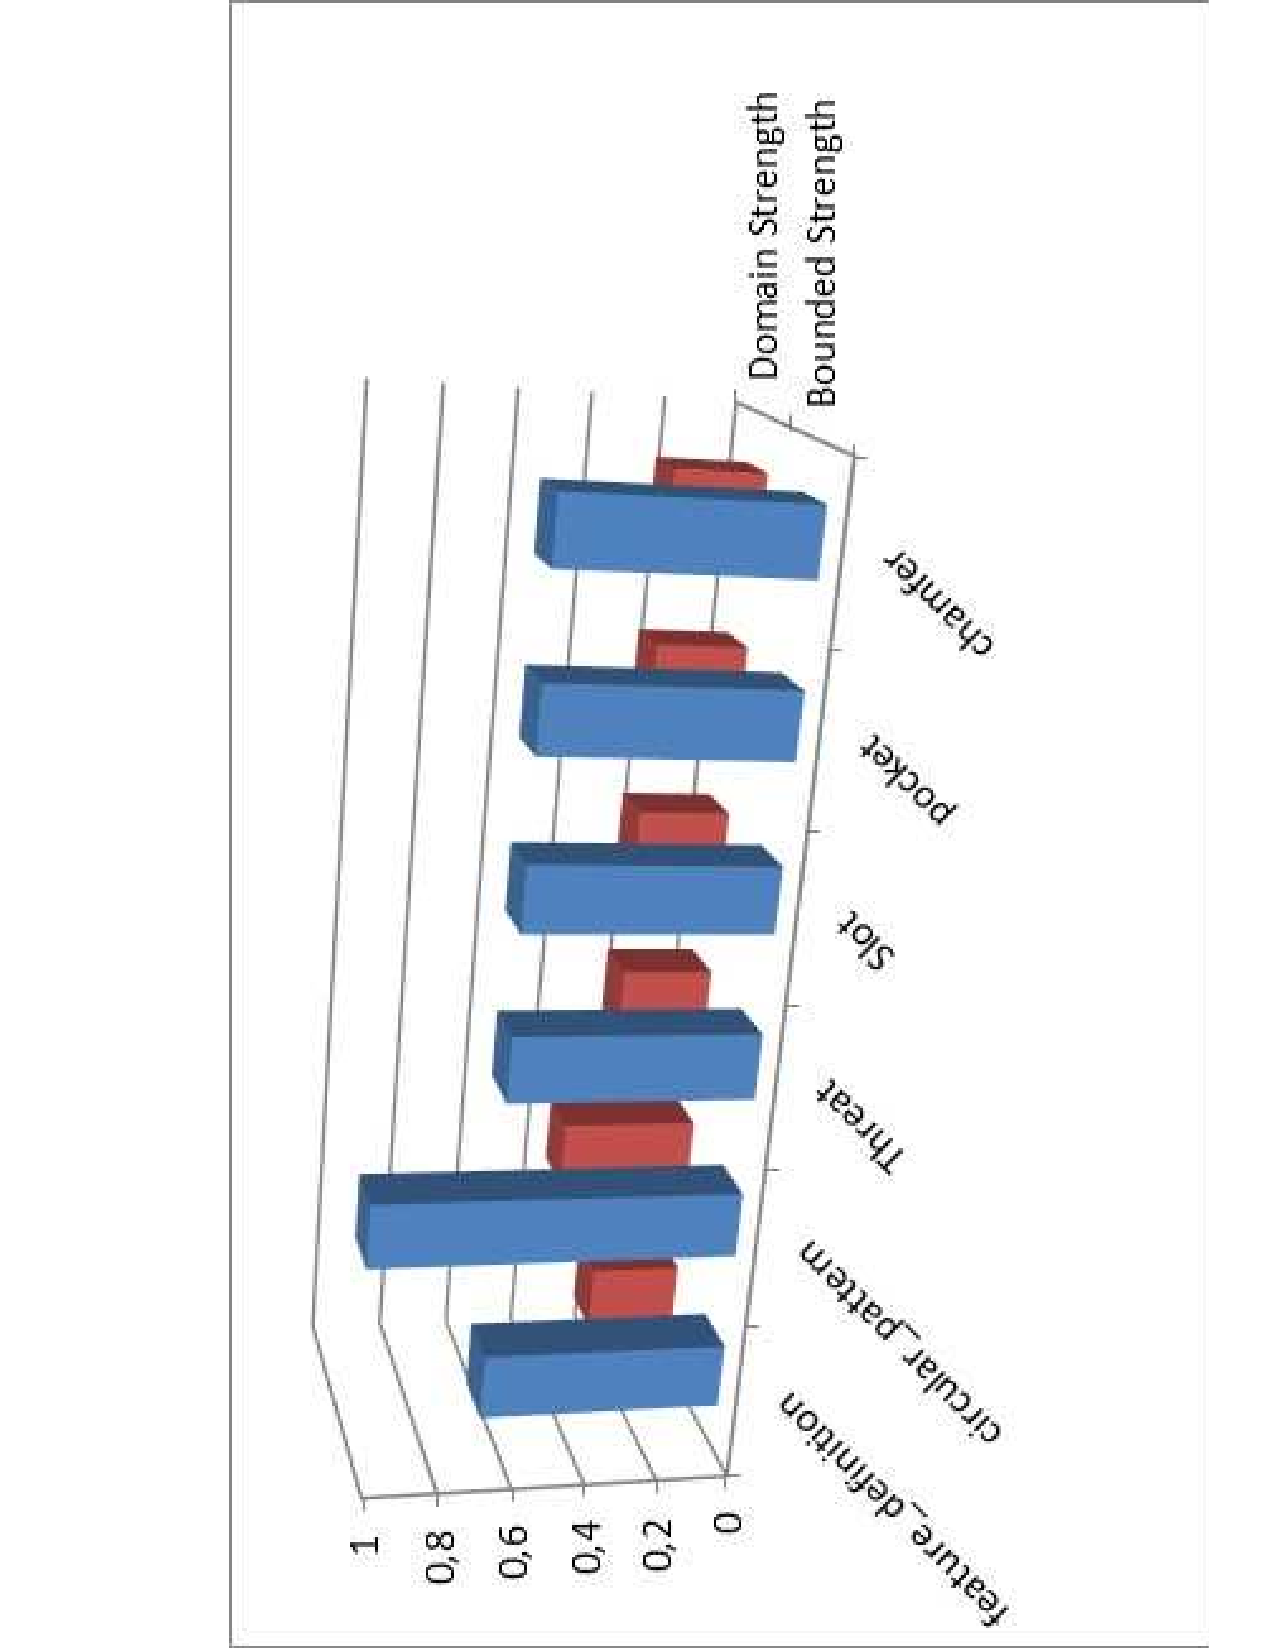
\includegraphics[scale=0.5, angle=-90]{figure-chapterIV/fig4-24.pdf}\\
	\caption{Hypermodule Resources}
	\label{figure4-24}
\end{center}
\end{figure}

\begin{figure}
\begin{center}
	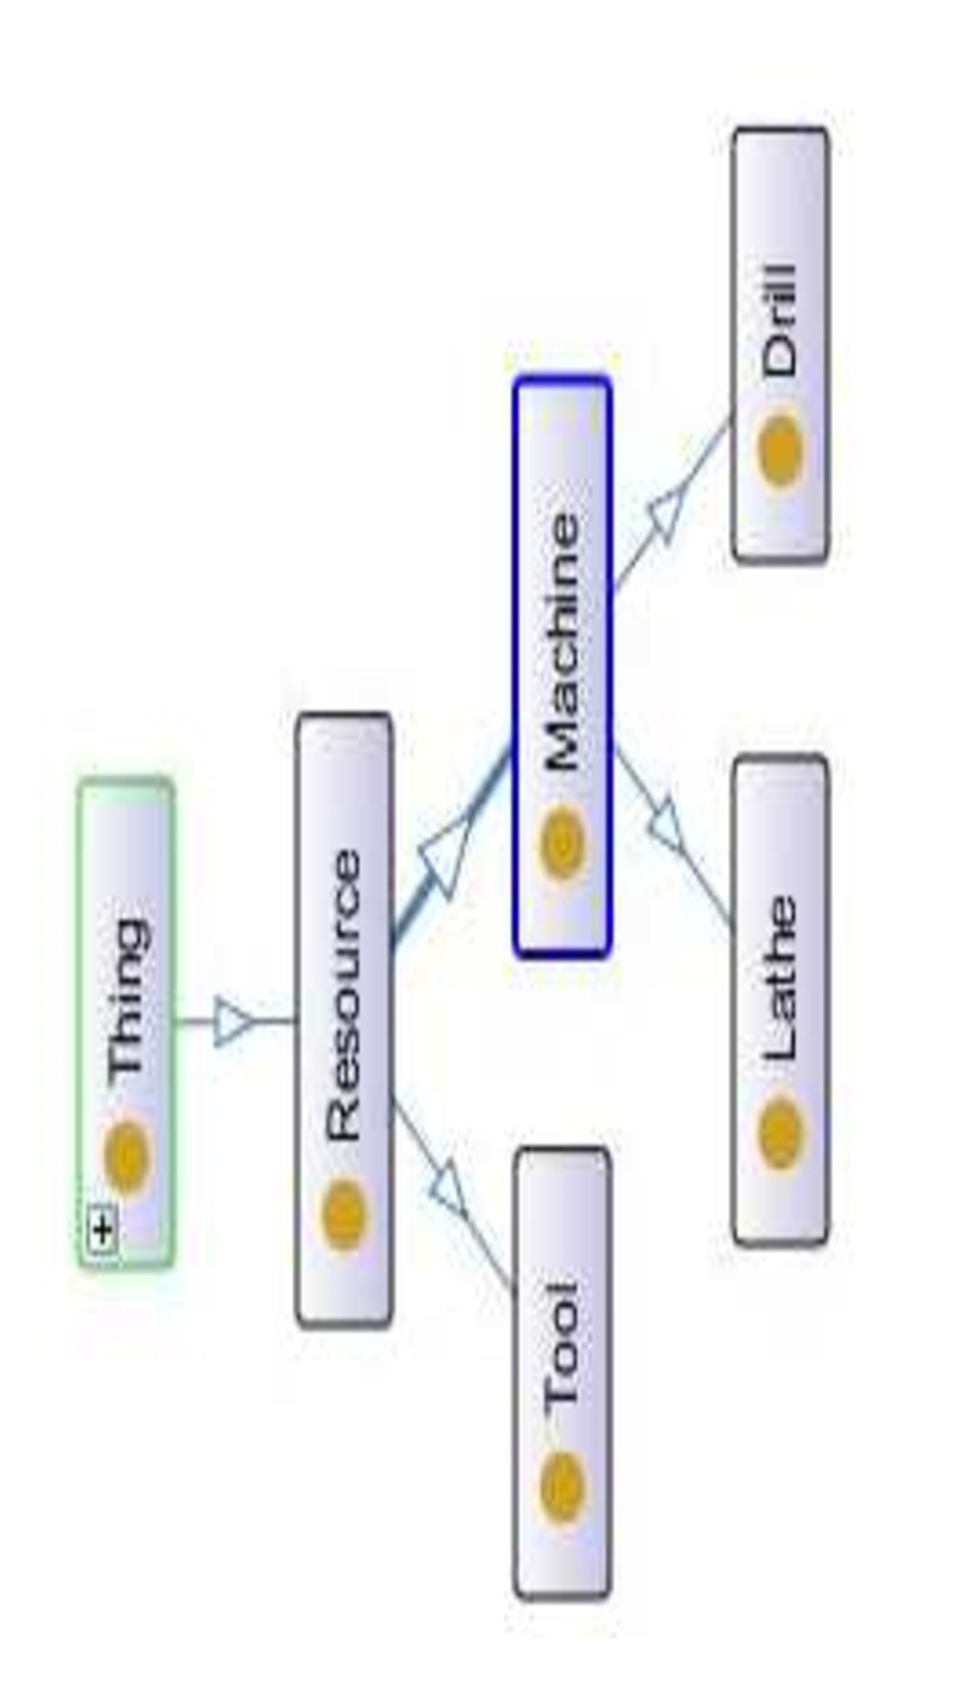
\includegraphics[scale=0.5, angle=270]{figure-chapterIV/fig4-25}\\
	\vspace{-40mm}
	\caption{Hyperontology of Resource}
	\label{figure4-25}
\end{center}
\end{figure}

\subsubsection{Hyper module of Curve}\label{subsubsection4.2.5.5}


The last hyper module we found following the proposed algorithm, corresponds to the  \texttt{Line, Conic, Curves, Circle, Hyperbola, Ellipse} and \texttt{Parabola} concepts. The mappings found correspond to 2 ontologies only, those are OntoStep and BeyondSTEP, while the other ontologies of the network remain isolated. 

In this case, the \gls{bs} of every concept is equal to 1, meaning that every concept is in all ontologies of the boundary, and  \gls{ds} is equal to 0.25 which means that these concepts make up less than 25\% of the ontologies. Fig. \ref{figure4-27} introduces the categorization of these concepts. Considering \texttt{Line} and \texttt{Conic} as \texttt{Curves}, and \texttt{Circle}, \texttt{Hyperbola}, \texttt{Ellipse} and \texttt{Parabola} as \texttt{Conics}. 



\begin{figure}
\begin{center}
	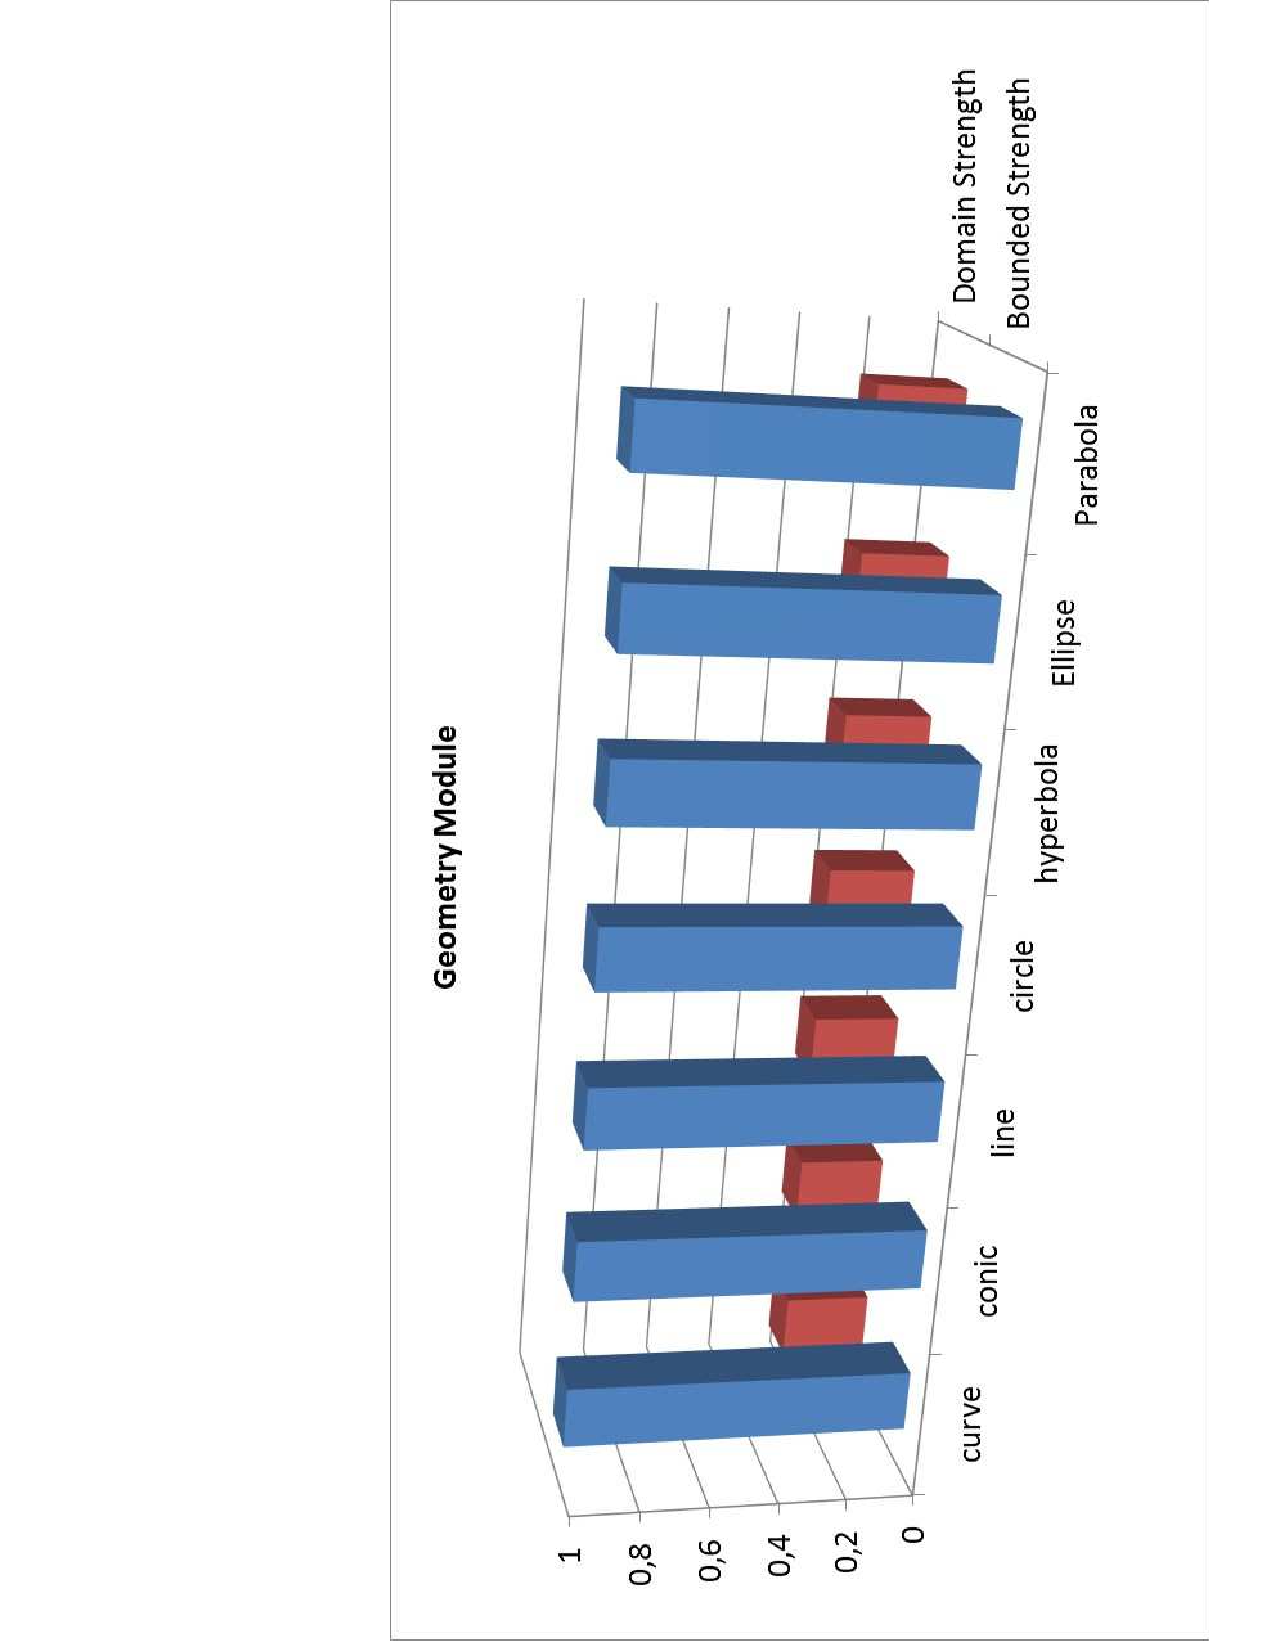
\includegraphics[scale=0.5, angle=-90]{figure-chapterIV/fig4-26}\\
	\caption{Geometry Hypermodule}
	\label{figure4-26}
\end{center}
\end{figure}





\begin{figure}
\begin{center}
	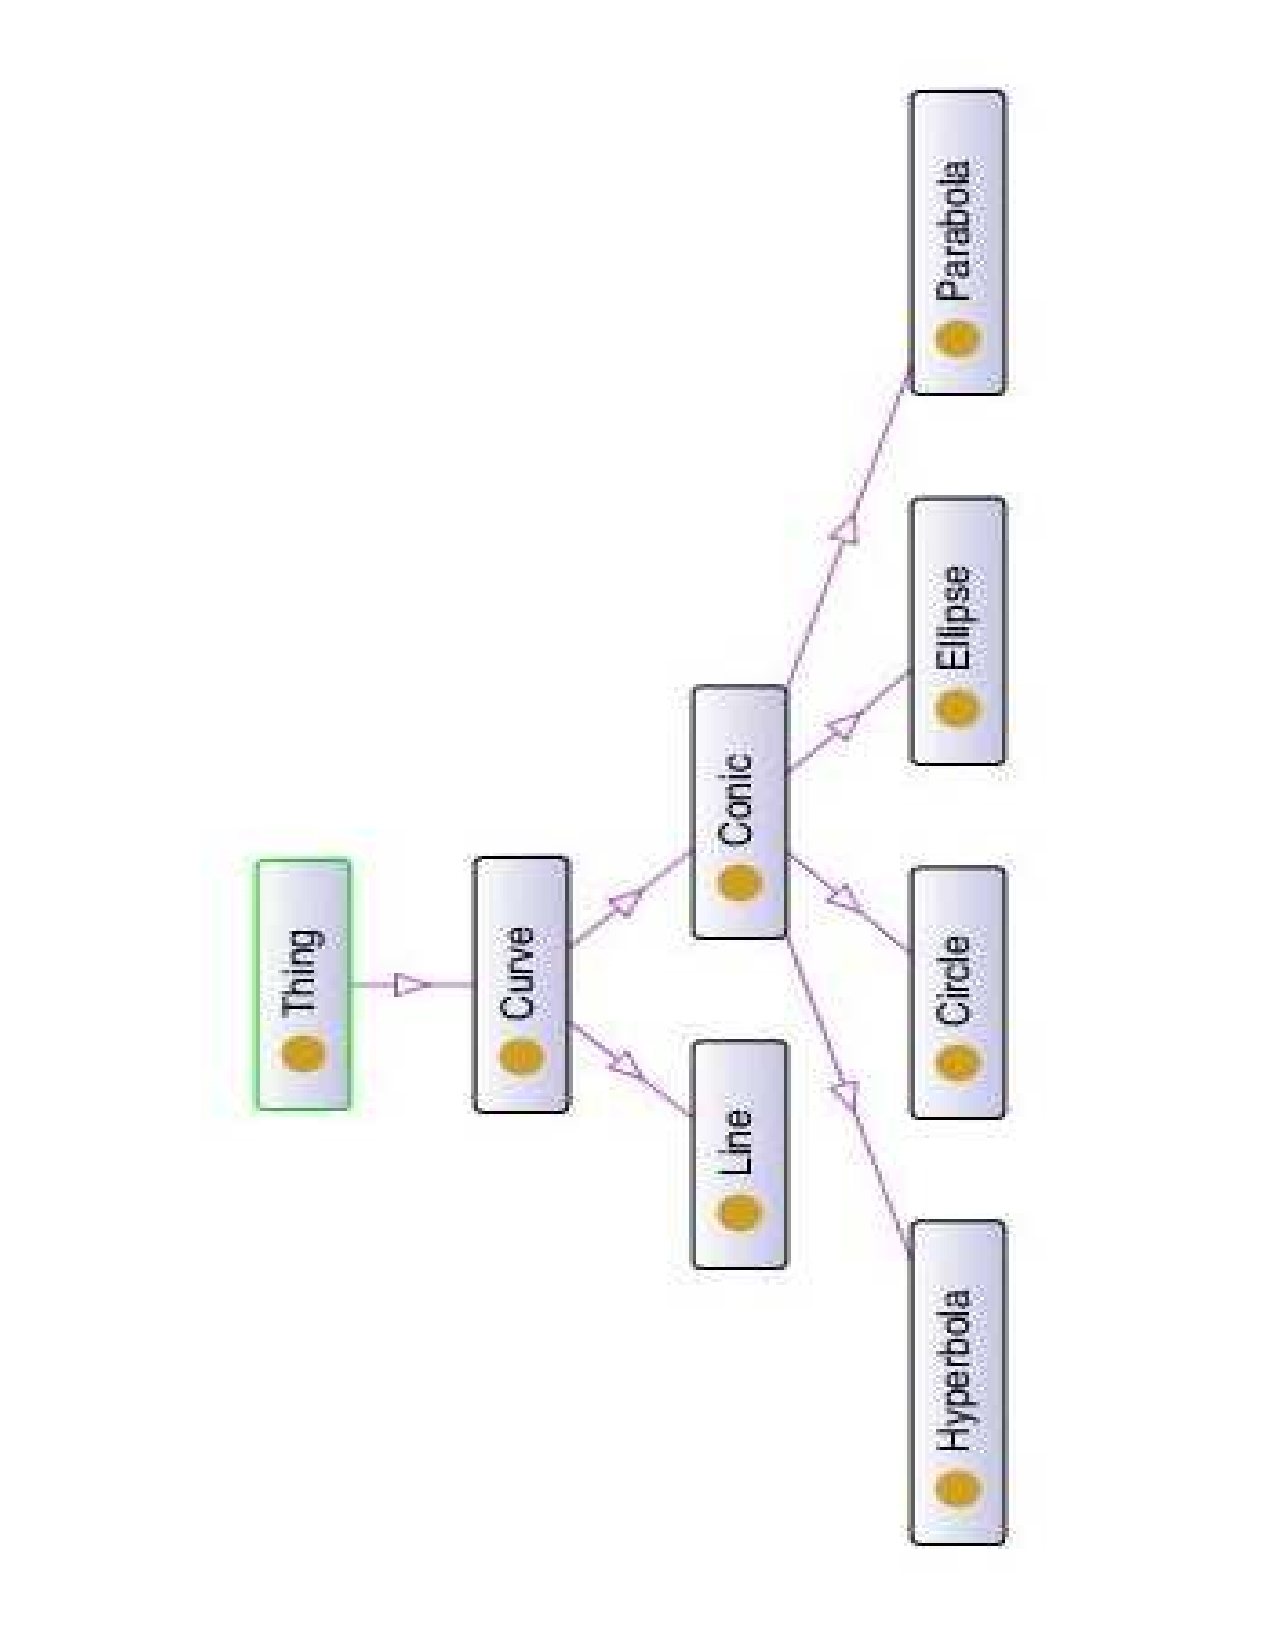
\includegraphics[scale=0.5, angle=270]{figure-chapterIV/fig4-27}\\
	\vspace{-20mm}
	\caption{Geometry Ontology}
	\label{figure4-27}
\end{center}
\end{figure}




With the hyper module of curves we complete the application of the algorithms proposed in Onto\textit{Smart}. The obtained hyper modules now have to be integrated with the network of ontologies shown in Fig.\ref{figure4-10}. At this point it is worth remarking that our hyper ontology will be formed by some hyper modules, and in the case of our algorithm we have proposed two types, mono-modules and multi-modules. This Hyperontology is an interoperability artifact that is located on top of the network of ontologies, and the mappings obtained from the algorithm serve as hyperlinks. With these notions we proceed to summarize our findings in Fig. \ref{figure4-28}, which at the same time serves as the representation of our complete Hyperontology. At the bottom of the figure, we show the network of ontologies from Fig. \ref{figure4-10}. At the top, every Hypermodule is drawn; the mono-modules containing only one concept in yellow, and the multi-modules containing several concepts in black. 


This figure illustrates the complexity of representing a domain of discourse, concretely considered in this case for manufacturing. For instance, a product can be goods or  service. If we choose to represent goods, some products could be represented as a \gls{cad} drawing, while others, like liquids, cannot be represented in this way. In the case of the resulting hyper ontology, it will only serve for representing solids according to the Features terminology it contains.

Furthermore, it is likely to find at least two   ontologies with restricted scope. Those include, for example, the Sweet Ontology, which only has a mapping through the hyper module of \texttt{Unit} toward 4 more ontologies, and BeyondStep which has two mappings through the concepts \texttt{Features} and \texttt{Geometry} toward 3 more ontologies. Such mappings allow us to extend those apparently restricted scope  ontologies through these mappings toward more complex ontologies.

Moreover, if we consider ontologies with an apparently  different scope in a manufacturing domain, like \gls{mason} (manufacturing) and GoodRelations (ecommerce), their commonalities allow certain information exchange through this network, in this specific case information about the product. In contrast, information of the manufacturing process is not exchangeable because these concepts are not part of GoodRelations terminology. 

Here we complete the activities of modularization planned in our methodology, before proceeding onto the steps of Axiomatization and Heterogeneity. Moreover in Section \ref{section4.4} an application example with the obtained hyper ontology in Fig. \ref{figure4-28} will be introduced. 



\begin{figure}

\begin{center}
	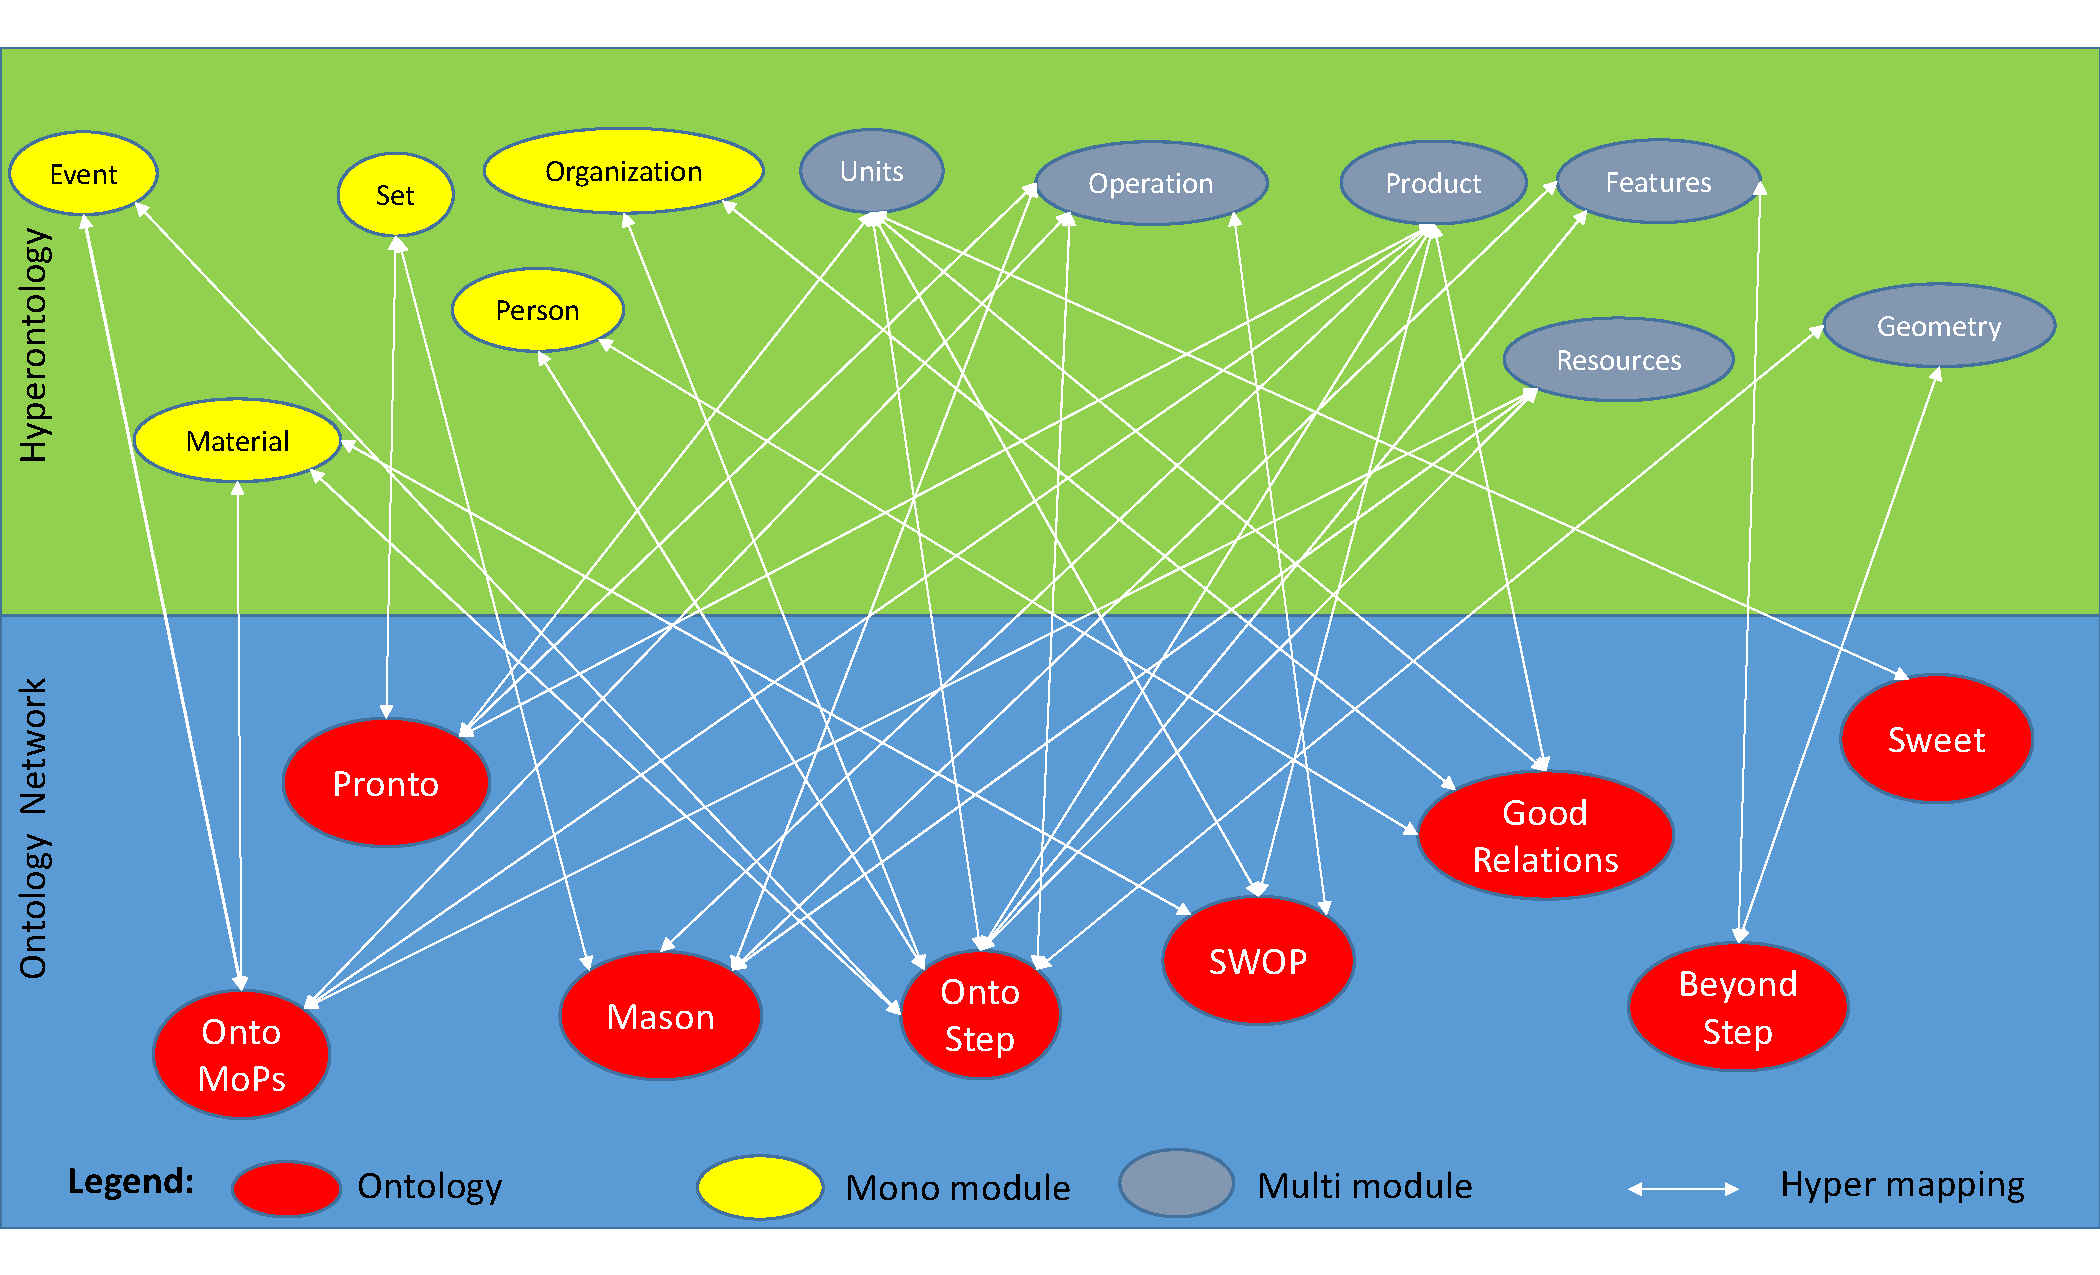
\includegraphics[scale=0.6, angle=90]{figure-chapterIV/fig4-28.pdf}\\
	\caption{Resulting Hyper ontology}
	\label{figure4-28}
\end{center}
\end{figure}



\section{Between Light Weight and Heavy Weight Ontologies}\label{section4.3}


Continuing with the development of our methodological approach as depicted in Fig. \ref{figure3-1} of our Proposed Methodology, we have to proceed to determine whether or not heavyweight ontologies are required, following the procedure indicated in Subsection \ref{methodology}. In this stage we applied the metric $al$ which lets us know the average of defined concepts in an ontology; moreover we proposed a criterion to determine whether or not a heavyweight ontology is required in our application\footnote{https://github.com/luisenriqueramos1977/OntoSmart/wiki/Axiomatization}. 

Following the proposed criteria, first it is necessary to determine whether heavyweight ontologies are needed, which depends of the application requirements. Thus we have to consider the following aspects: All ontologies considered in Fig. \ref{figure4-28} were written in  \gls{owl} and \gls{owl} is based in \gls{owa}, which means an individual is considered as a member of a concept, and it is necessary to provide a specific definition of the concept or restrictions through  closure axioms. These closure axioms allow the classification of individuals as members of a class. This classification feasibility is a fundamental characteristic in Ontological Engineering.  

To illustrate this classification need in engineering, we can   consider the \gls{afr} approach, which consists in recognizing certain features from \gls{cad} files. In the hyper module of Features, some of the most common mechanical features mentioned in the literature are included. When \gls{afr} is executed on a digital design, the following classification takes place: a group of geometrical elements receive mechanical and manufacturing semantics when they are classified according to some specific features, defined by a set of axioms. 

There is also the \gls{fms} approach, which assumes that with an intensive utilization of Numeric Control (NC) techniques, automatic materials handling and computer hardware and software, the manufacturing time for customizing goods should be considerably reduced. Here a classification is also involved whenever from a group of resources (machinery) we have to decide which can fulfill our manufacturing requirements   and how they should be organized in the factory. 

Another example can be provided considering market segmentation principles. In this case customers are divided into groups or segments, based on their preferences, and products can be assigned to certain segments of customers according to the satisfaction levels they are able to provide for each group or segment. 

Through the description of the three common scenarios mentioned above, we can consider that heavyweight ontologies are required in such scenarios in order to enable classification. 

After defining the requirement of heavyweight ontologies for manufacturing, we applied the formula proposed in Onto\textit{Smart}\footnote{shorturl.at/oI347} to obtain the relation between defined and primitive concepts in an ontology, with the intention of defining the purpose of the evaluated ontology, controlling vocabulary or classification.  Thus, we can confirm our position that manufacturing ontologies should have mostly defined concepts with the intention of making such ontologies usable.   



\begin{figure}
\begin{center}
	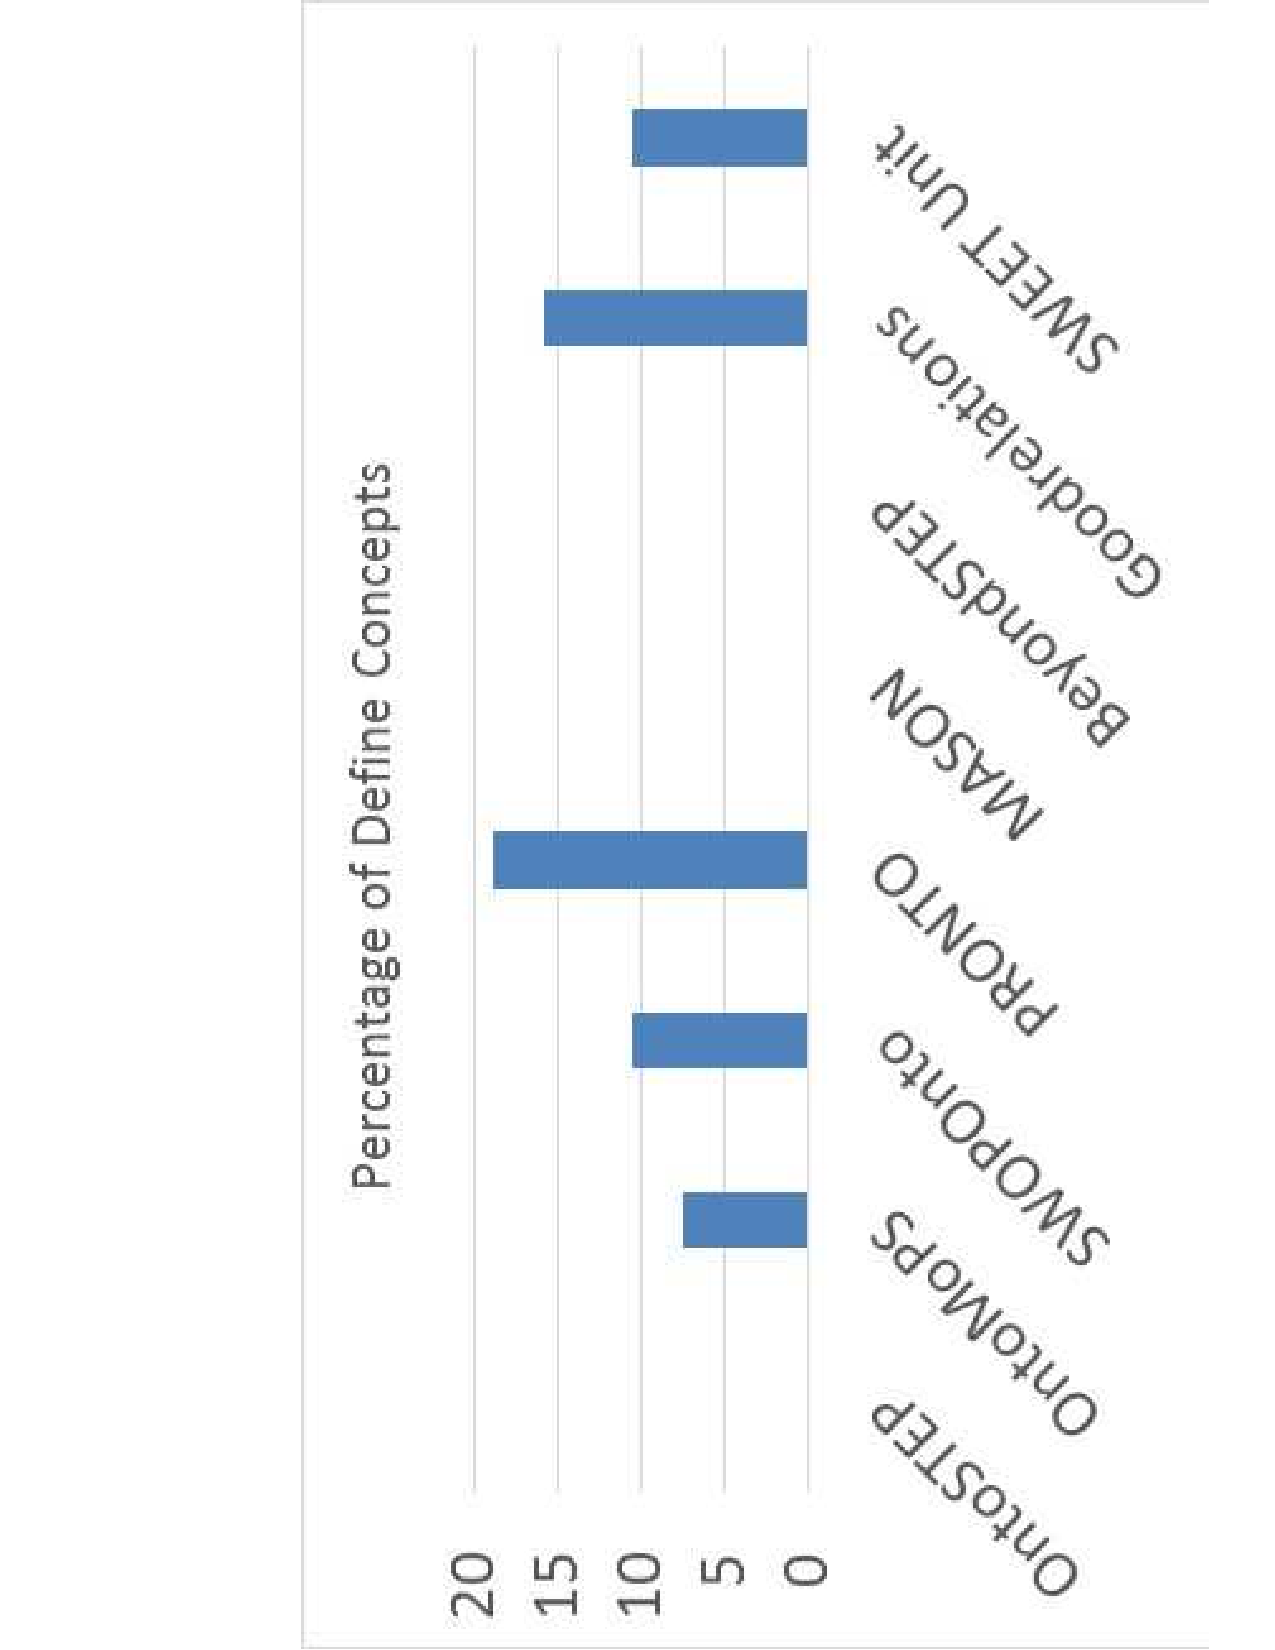
\includegraphics[scale=0.5, angle=-90]{figure-chapterIV/fig4-29.pdf}\\
	\caption{Defined    Concepts in Network}
	\label{figure4-29}
\end{center}
\end{figure}



Fig. \ref{figure4-29} presents a view of the presence of defined concepts in the network of ontologies under evaluation. From the 8 ontologies considered, 5 have some defined concepts in different proportions, varying from 7 to 19\% of the total. Here, an apparent contradiction appears: that is while in the previous paragraph we stated that heavyweight ontologies are needed for applications like \gls{afr} and \gls{fms}, Fig. \ref{figure4-29} shows that in many ontologies like OntoSTEP, \gls{mason} and BeyondStep, there are no defined concepts. However, in other ontologies like \gls{pronto} and GoodRelations there are defined concepts present,  ranking from 15\% to 19\%.

To relate usability with heavyweight ontologies, we consider the result obtained in the case of the GoodRelations ontology, because from ontologies mentioned in Fig. \ref{figure4-29} only this has shown use outside of academia. This ontology is used in some of the most important   search engines and it is well accepted in the ecommerce community \cite{hepp_references_2013}. Moreover it has an appropriate platform for making it available to a community of users. Approximately 16\% of this ontology is made up of defined terms, and its basic use consists in allowing goods selection according to user criterion. 

Another necessary consequence of this result can be concerning OntoStep and BeyondStep. From the percentage of defined concepts in OntoStep and BeyondStep shown in Fig. \ref{figure4-29},  we can assure they are lightweight ontologies because they contain no defined concepts. Thus, if we wish to perform \gls{afr}, many terms in these ontologies shall be defined, in other words OntoStep and BeyondStep, are incomplete for \gls{afr} and \gls{fms}, and the Ontological Engineer will need to perform additional work defining concepts to make these ontologies usable with this type of tasks. 

In this Subsection we discussed axiomatization requirements, and showed that from the list of ontologies we have evaluated, many were lightweight. This result does not make these ontologies useless, but it does make necessary additional work to define appropriate concepts in order to make them usable in tasks like \gls{fms} and \gls{afr}. For these tasks, in our opinion, heavyweight ontologies are required. 

Following with our methodology shown in Fig. \ref{figure3-1}, we proceed to the heterogeneity activities. However as we will later demonstrate, this decision is based on application requirements, so in the next Section we present an application example where domain requirements will take us back to heavyweight ontologies in order to fulfill the application goals.  



\section{Implementing Heavyweight Ontologies}\label{section4.4}


At the beginning of report, \gls{cax} systems were introduced as an attempt to improve manufacturing automation, optimization and acceleration levels. For example, during this research we observed how AutoDesk developed its \gls{dxf}, a \textit{de facto} standard for the exchange of \gls{cad} data facilitating reading a \gls{cad} design previously deployed using other software tools such as AutoCAD® of AutoDesk. A detailed explanation of this standard can be found in the \gls{dxf} Reference Manual \cite{autodesk_dxf_2009}.  This standard defines geometric primitives such as LINE, CIRCLE, ARC and ELLIPSE entities. A group of codes is specified for each one, indicating what type of data value or feature they follow. It is also possible to extract from a \gls{dxf} file descriptions of text, surfaces, color and texture, but the information on solids is encrypted \cite{choi_exchange_2003} and limits data information exchange among \gls{cad} design. In the same way, the work flow starting from the manufacturing design is restricted to the AutoDesk family of products. Therefore, besides the important advantage of \gls{cax} systems, these technologies have shown patent shortcomings, one of these is the lack of interoperability.  This interoperability issue occurs because most vendors allow interoperability along the workflow of the tools they offer, but interoperability between tools of different vendors tends to be limited in some way.


In recent years there has been a movement toward the utilization of the ontological approach in engineering applications for the representation of  \gls{cad} models to capture feature semantics and to use such models among different systems maintaining the designer’s purpose. \cite{abdul-ghafour_common_2007} presented an architecture for a Data Exchange among different \gls{cad} software tools, where ontologies are proposed to represent terminologies of several commercial \gls{cad} software tools, and a main ontology would serve as a Common Design Feature Ontology. \cite{abdul-ghafour_common_2007} proposed to write and store ontologies of each \gls{cad} system using \gls{owl}, generating ontologies of such systems.   These ontologies have to be mapped into a Common Design Ontology to make them interoperable across different software applications. Similarly, \cite{andersen_building_2007} proposed an ontology of \gls{cad} model information; this proposal is described as an introduction to ontologies and shapes representation and deals only with the STEP standards as also done by \cite{abdul-ghafour_common_2007}, presenting a taxonomy of terminologies included in the STEP standard. 

In contrast, building on the proposal of \cite{abdul-ghafour_common_2007}  we  have proposed a different data exchange approach \cite{ramos_ontological_2010}. There, intermediate ontologies were avoided and a general \gls{cad} terminology was used without adopting specific standard \gls{cad} terminology. We considered this could be a disadvantage for an approach that, on the one hand, claims to be ontological while, on the other hand, it is only being related to one \gls{cad} standard. Fig. \ref{figure4-30} presents our first attempt to deal with this interoperability issue in \gls{cad}.  In this figure, we exemplify the architecture with \gls{dfx} and \gls{iges} standards. Consequently, in the figure  there are four parsers: Two preprocessors parsers for exchanging \gls{dfx} into \gls{owl}, and two postprocessors parsers for exchanging \gls{owl} in \gls{dfx}, similarly in \gls{iges}. As soon as a standard is converted into \gls{owl}, the reasoning framework of the Semantic Web becomes available. With a \gls{cad} design based on \gls{owl}, it is possible to provide reasoning on the \gls{cad} ontology, in order to exchange from one format to another. 


\begin{figure}
\begin{center}
	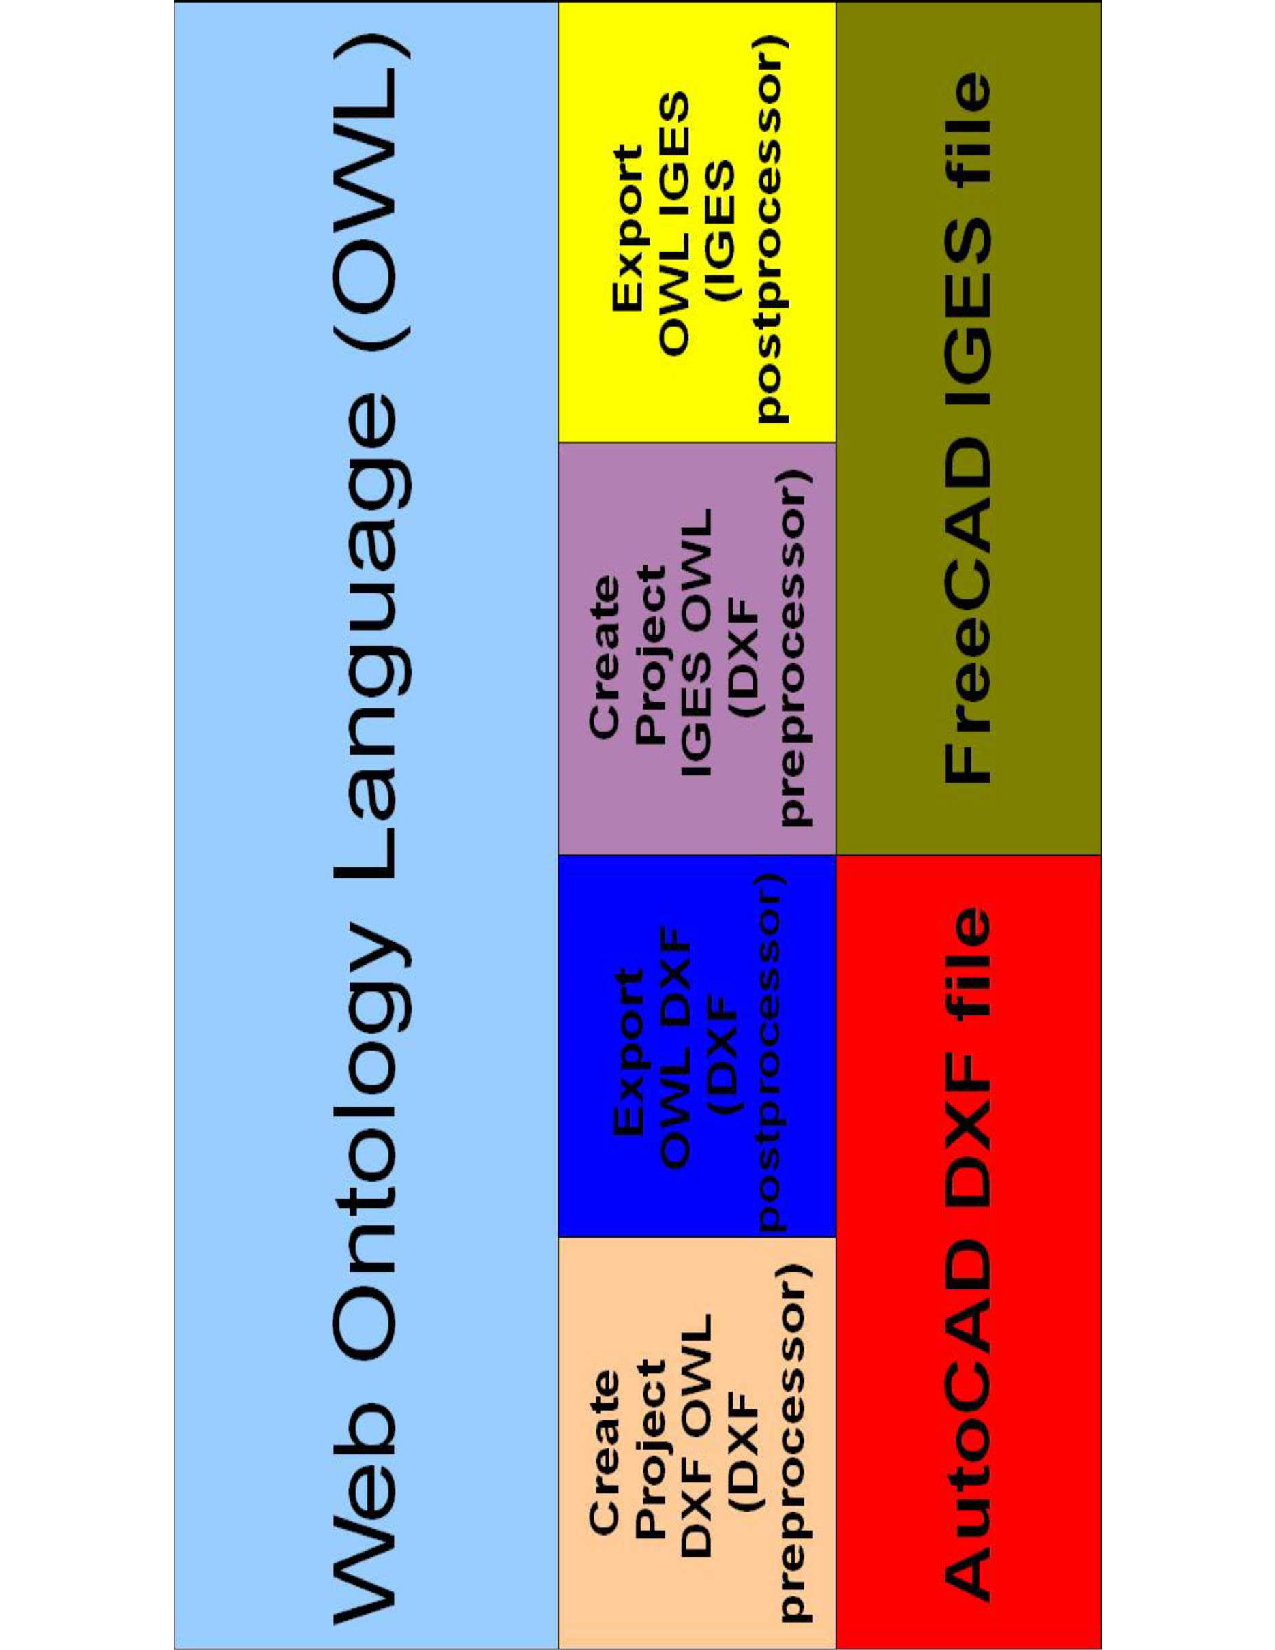
\includegraphics[scale=0.5, angle=270]{figure-chapterIV/fig4-30}\\
	\caption{\gls{owl} Based \gls{cad}   Exchange Framework}
	\label{figure4-30}
\end{center}
\end{figure}

In order to assess the usability of the Semantic Web in manufacturing, other uses additional to exchanging data of specific \gls{cad} formats like \gls{dxf} and \gls{iges} shall be considered. The issue of representing and reusing the designer’s purpose in a \gls{cad} designs is one of those. This issue is illustrated in Fig. \ref{figure4-30} and Fig. \ref{figure4-31}. The former shows a common mechanical piece used in engineering, better known as a flange. The latter shows the same piece obtained by automatically parsing a \gls{dfx} file into a \gls{cad}–\gls{owl} file generated by means of a plug-in called “\gls{cad} Viewer Tab”, which we developed as part as our previous work related with this research. This plug-in was integrated in Protégé. This plug-in implements the procedure   of our proposed architecture, specifically the “Create Project \gls{dfx}  \gls{owl}” parser shown in Fig. \ref{figure4-30}.

Even though both figures seem to have the same representation of a mechanical piece, they are actually not the same. Only primitives (circles) are what have been actually exchanged from AutoCAD into \gls{dxf}, and so into \gls{owl}. This means that while the viewer may perceive a flange, for the computer they just remain as circles. Thus design purpose (knowledge) is lost during the exchange due to missing semantics.



\begin{figure}
\begin{center}
	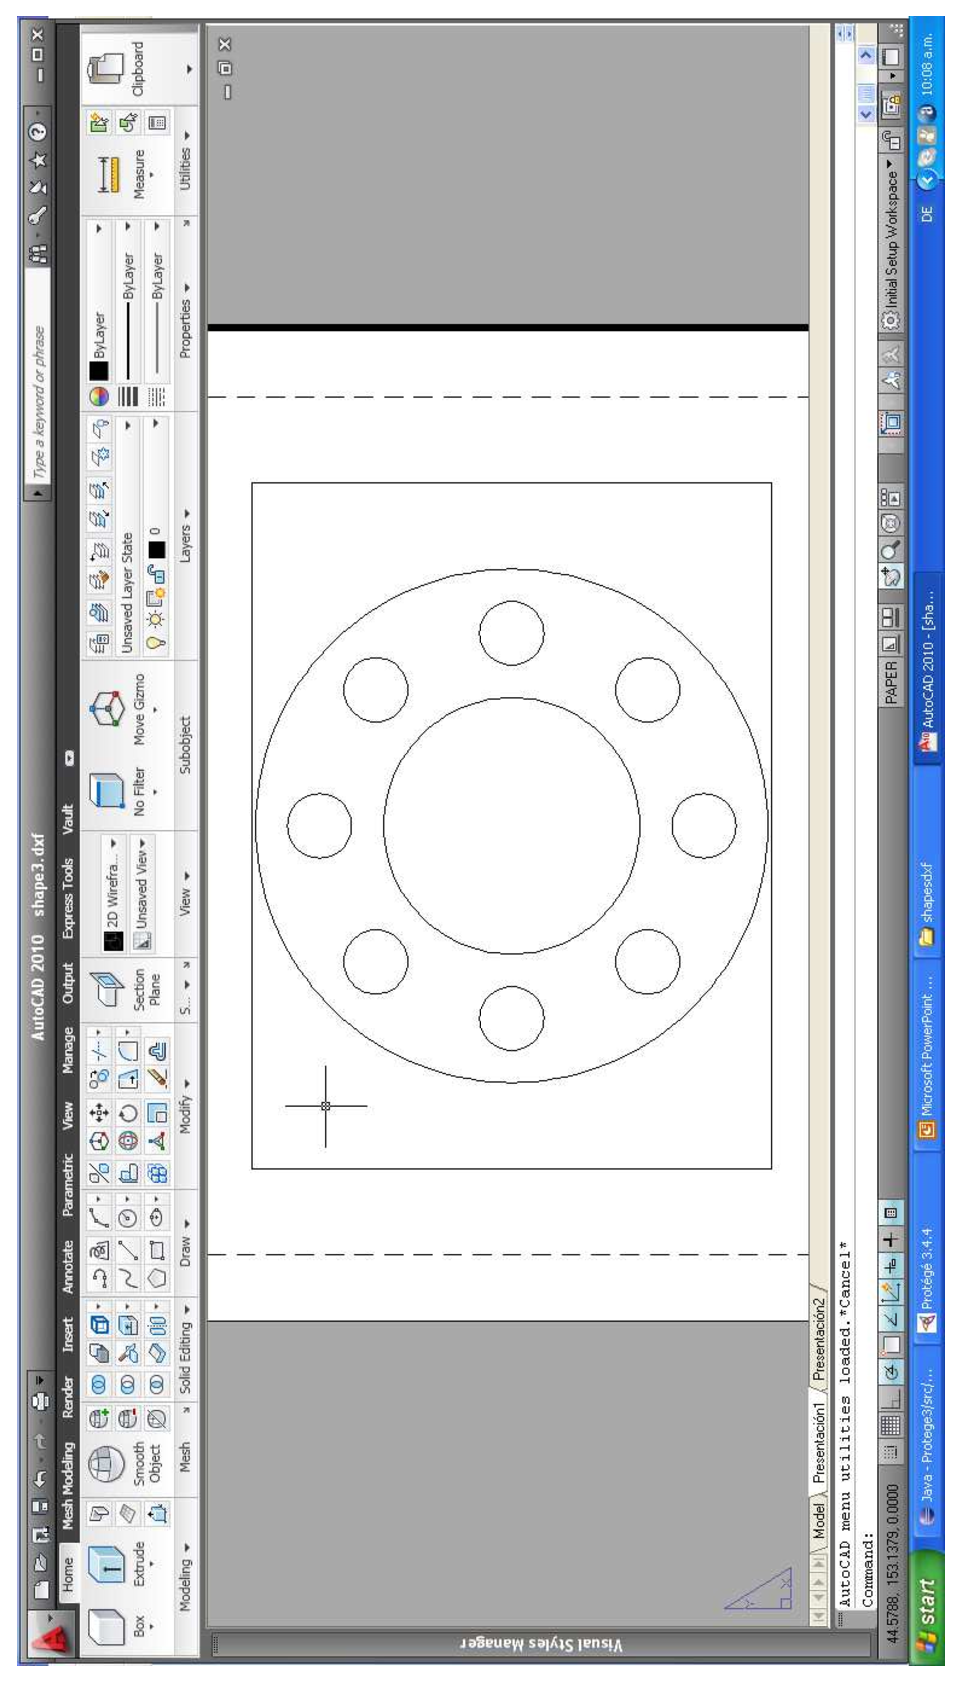
\includegraphics[scale=0.5, angle=270]{figure-chapterIV/fig4-31}\\
	\caption{Shape in AutoCAD}
	\label{figure4-31}
\end{center}
\end{figure}





\begin{figure}
\begin{center}
	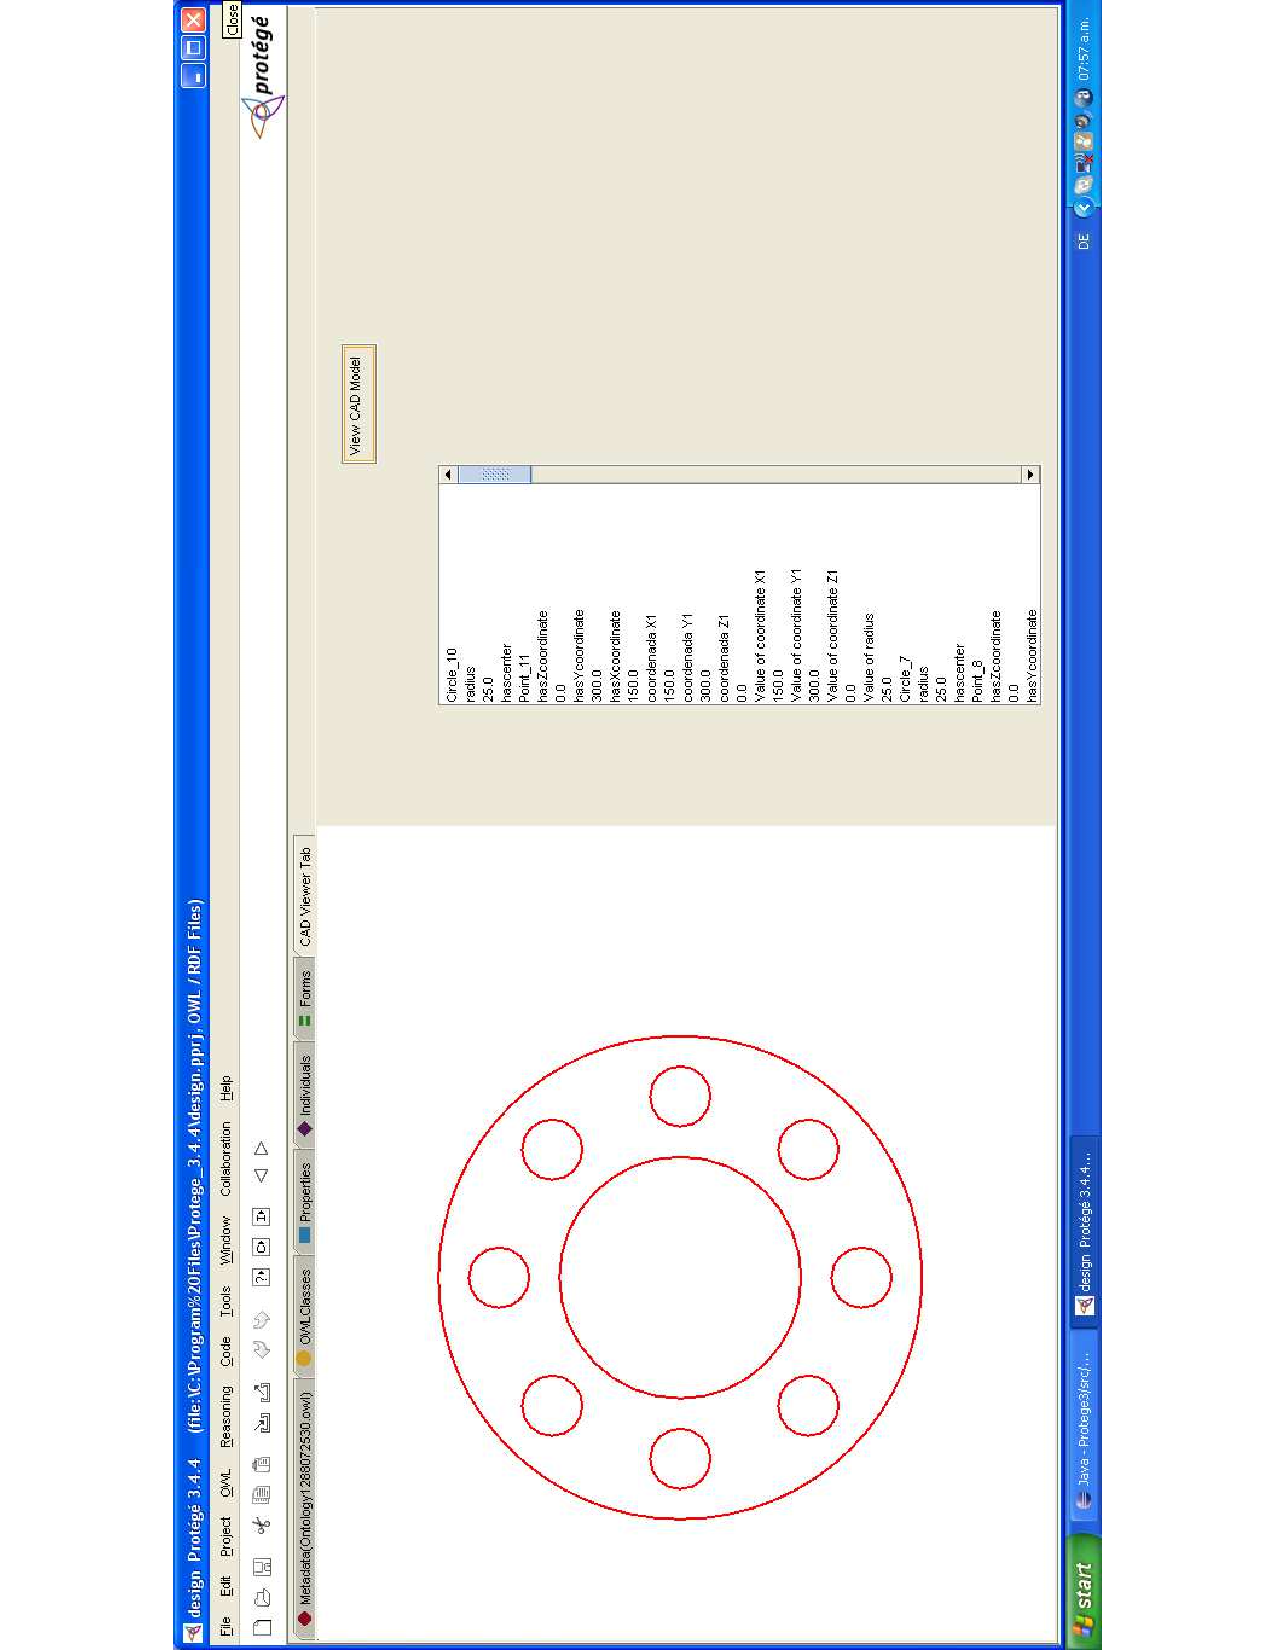
\includegraphics[scale=0.5,angle=270]{figure-chapterIV/fig432}\\
	\caption{Shape in OntoCAD}
	\label{figure432}
\end{center}
\end{figure}


In order to recover the designer intent, it is necessary to provide tools or representations to capture the designer’s knowledge. Moreover, it would be appropriate to support the knowledge of the manufacturing engineer, quality control, and other related tasks as well. 

Fig.\ref{figure4-33} illustrates how we consider Semantic Web Technologies should be ordered in a general framework to make the requirements mentioned in the previous paragraph. Going into details, in Fig.\ref{figure4-33} we propose a foundation of the initial architecture.

In the middle of the architecture, we placed Semantic Web technologies for 2D, and a 2D features ontology. Thus, primitives can be interpreted as features, and quality control can be applied to them. At the top of the architecture, Semantic Web technologies adapted for 3D interpretation are included. A GUI was developed in order to allow visualization of the design. Although this framework apparently covers the aforementioned requirements, we want to introduce a more technical example to view detailed limitations of  the \gls{owl}  language for representing certain manufacturing scenarios, and to link it to our evaluation and definition of the above hyperontology.


\begin{figure}
\begin{center}
	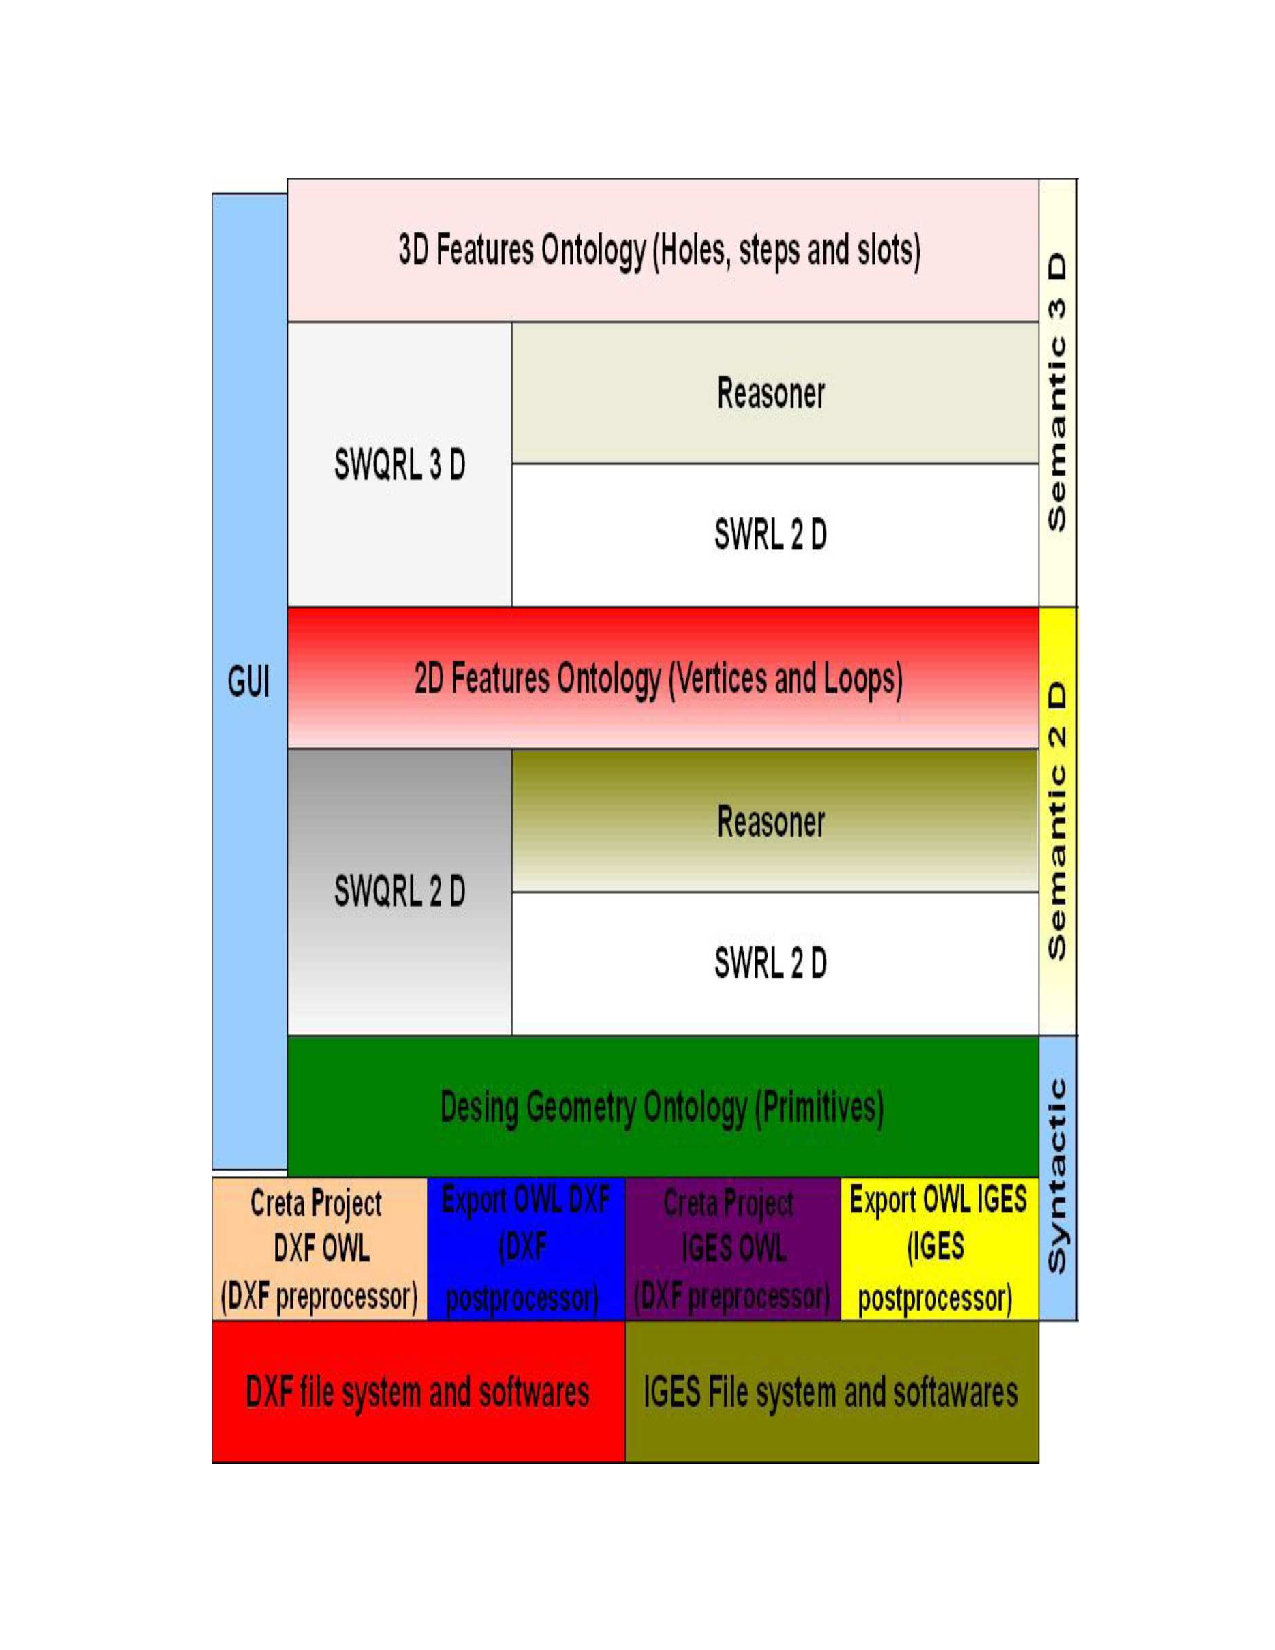
\includegraphics[scale=0.8]{figure-chapterIV/fig4-33}\\
	\vspace{-40mm}
	\caption{OntoCAD Framework}
	\label{figure4-33}
\end{center}
\end{figure}

As we mentioned in the previous paragraph, we want to introduce a more technical example from the manufacturing point of view, in order to require the major expressiveness of \gls{owl}. Such an expressiveness level demand can be found even in the manufacturing process of 2D design. Sheet   metal parts are some of these. These elements are commonly used in several products manufactured in modern industry: aerospace, automotive, appliances, machine tools, etc. are only some of these. Although various software tools are available for making digital designs for such metal parts, trying to use those designs as input for process planning and manufacturing is not simple.  The majority of standards for \gls{cad} do not represent the particular features required when manufacturing. For instance, declaring when a circle corresponds to an inner edge or an outer edge has significant consequences during manufacturing, although this may not be necessary when displaying designs. Allowing interoperability across the \gls{cad}-\gls{cam} process should enable designers to select optimal manufacturing conditions. For instance, to choose a sheet thickness that would prevent crashes when punching holes.


In order to achieve such interoperability, manufacturing features must be extracted from \gls{cad} files.  Extracting these features demands identifying certain patterns in the \gls{cad} files that shall receive additional manufacturing-relevant enrichment.  Information about features is further used to determine the machining tools and manufacturing processes required to manufacture a given design \cite{cayiroglu_new_2009}. Feature information can also then be used to pre-check designs in order to detect production rule violations. If these violations are not detected in an early stage of design, the life cycle of development increases, raising production costs and time to market \cite{radhakrishnan_design_1996}. Manual recognition of the targeted features is not a viable alternative, however: \gls{afr} is required. Nevertheless, even nowadays \gls{afr} is not fully integrated with \gls{cad} software tools. It is applicable only to parts with relatively simple geometry and still requires human intervention to obtain the features identified. Moreover, such techniques are generally supported only in expensive \gls{cad} software tools that are beyond the reach of small scale industry \cite{kumar_trends_2005}. 


In \cite{ramos_ontology-based_2011}   we proposed the partial application of the framework presented in Fig. \ref{figure4-33} in order to deal with the shortcomings of \gls{afr} from sheet metal designs and designs checking. This ontology-based framework should facilitate interoperability across the entire \gls{cad}-\gls{cam} process. Our system integrates both a \gls{cad} and a features ontology; these ontologies were written in \gls{owl} (Web Ontology Language) and represent 2D primitives as lines, arcs and circles in the \gls{cad} ontology and as edges, slots, tab and holes in the features ontology. In order to provide rules and query support, \gls{owl} was complemented with \gls{swrl} and \gls{sqwrl}. The result is an ontology-based system that allows us to automatically extract the most common manufacturing features referred to in the literature.


One of the main issues of \gls{afr} is the abstraction level involved in the manufacturing domain \cite{shah_functional_1988}. On the one hand, designers make designs from the functionality and usability point of view, with its own restrictions and rules. On the other hand, manufacturing engineers evaluate a design from the manufacturing point of view, considering factory constraints. This is mainly the reason why quite distinct standards, formats and tools have been developed. In the two domains, two different interpretations of the requirements take place for the same purpose, so an interoperability channel between them is needed.  This channel needs to enable the interchange of information of products as well as the evaluation of designing and manufacturing restrictions. 

In Fig. \ref{figure4-34}, we introduce the mapping architecture implemented for dealing with this situation. Knowledge transfer between domain ontologies was enabled by a third, mapping ontology, which keeps track of the related concepts of both domains. This mapping ontology was developed using the Prompt plug-in \cite{noy_prompt_2003}. This latter architecture can be considered as a simplified and specialized view of Fig. \ref{figure4-28}, where two terminologically similar ontologies, \gls{mason} and OntoStep were hypermapped with BeyondStep within a feature’s Hypermodule. Terms present in those ontologies are naturally related to the 3 dimensional domain given the relations found by the results obtained from the extraction of the feature’s hyper module, which was described in Section \ref{subsubsection4.2.5.4}. We want to remark that the application, based on the architecture depicted in Fig.\ref{figure4-34}, has a limited scope and it was developed as part of our initial experiences, while the Hyperontology proposed in Fig.\ref{figure4-28} has a large scope within the manufacturing domain. 

Moreover, Fig. \ref{figure4-34} makes evident how we deal with one of \gls{owl}’s shortcomings, which was the \gls{owl} limitation in performing inference over inferred knowledge. In other words, if in a given \gls{kb} we applied certain rules to determine the quality of a design, and we inferred the design or some parts of it are technically correct, the inferred design or its parts cannot be further reused, unless we record them as asserted knowledge into the same \gls{kb}. 

This \gls{owl} issue is also depicted in Fig. \ref{figure4-33} when we try to move upstream through the architecture, given that in the case of \gls{dxf} only primitives are exported in this format. Thus 2D features can be inferred in a first stage, but if we try to go forward for a 3D inference, it is necessary to recreate an environment to enable reusing the previously inferred knowledge. Such an environment implies mapping between  several ontologies as in the case displayed in Fig. \ref{figure4-34}. 


\begin{figure}
\begin{center}
	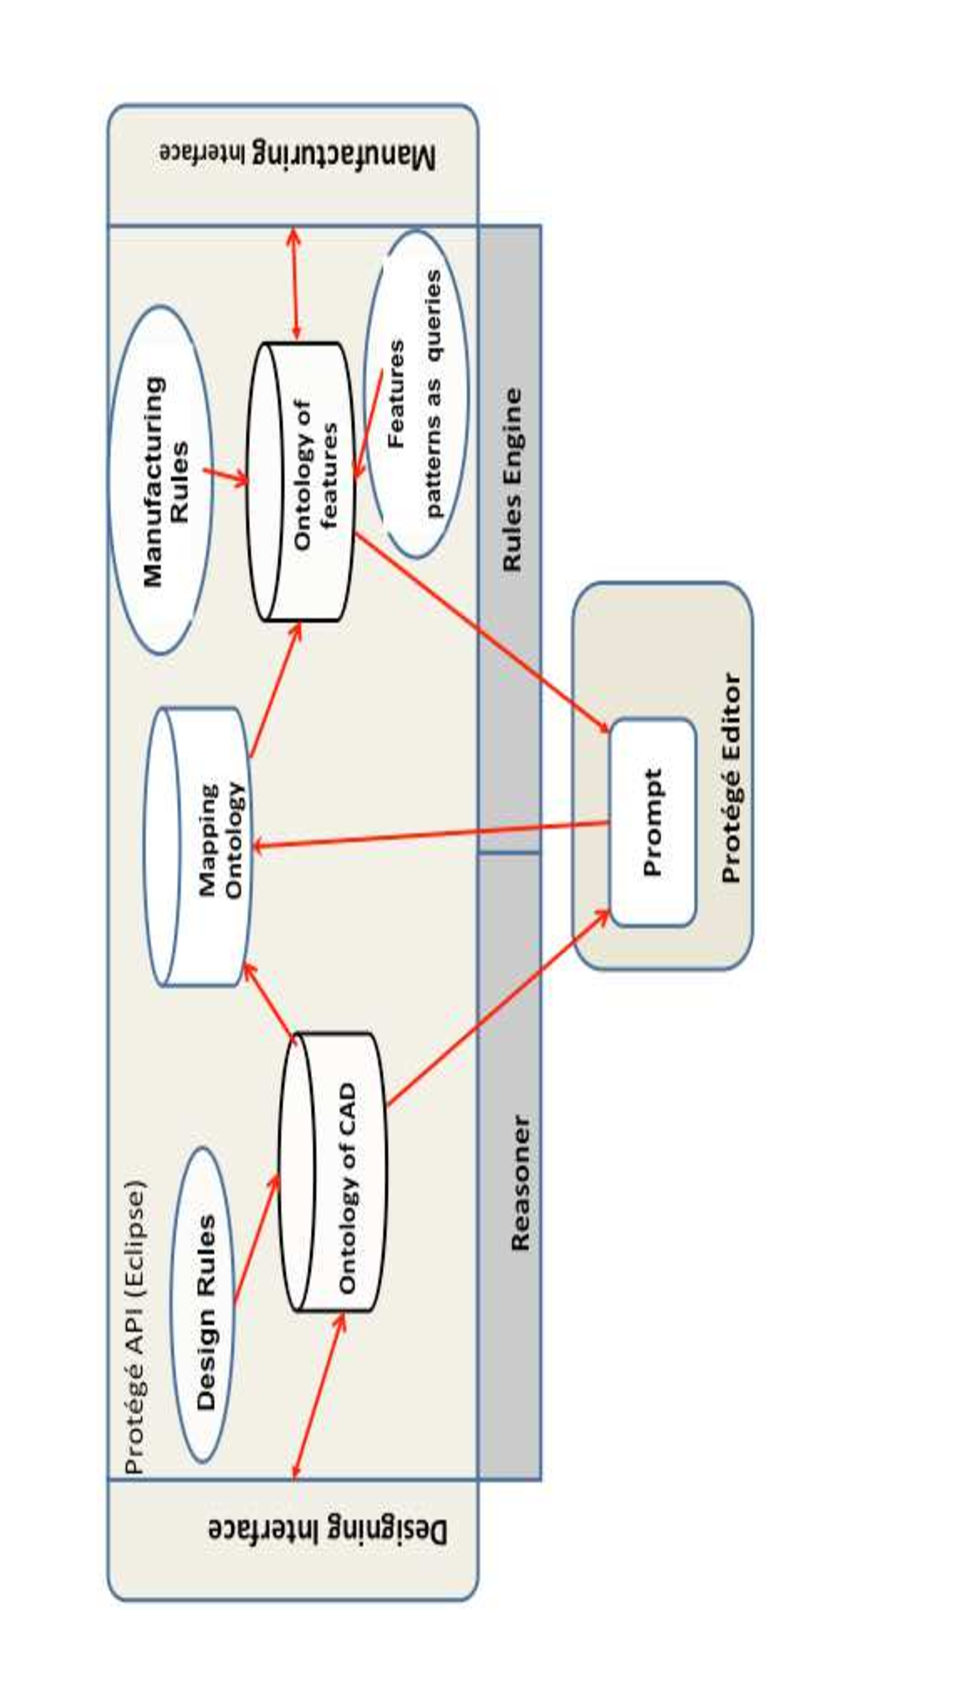
\includegraphics[scale=0.5, angle=270]{figure-chapterIV/fig4-34}\\
	%%\vspace{-60mm}
	\caption{Mapping Architecture}
	\label{figure4-34}
\end{center}
\end{figure}


For larger sets of ontologies, and with more complex tasks to perform, we can say that we are in the presence of a hyper-mapped architecture. For instance, manufacturing Operations, mentioned in Fig. \ref{figure4-28}, could be introduced in Fig. \ref{figure4-33} in order to deduce such operations for manufacturing the inferred features. Going into detail, Fig. \ref{figure4-41} lists most of the features mentioned so far, as well as the restrictions required to make them appropriate for manufacturing. Thus, after features are deduced, through the architecture suggested in Fig. \ref{figure4-34} inferred knowledge as features can be available to evaluated  them in order to determine their accuracy with quality restrictions. Every restriction illustrated in Fig. \ref{figure4-35} was successfully represented with \gls{owl}, and in all restrictions,    except Distance between holes, quality could be deduced. 



\begin{figure}
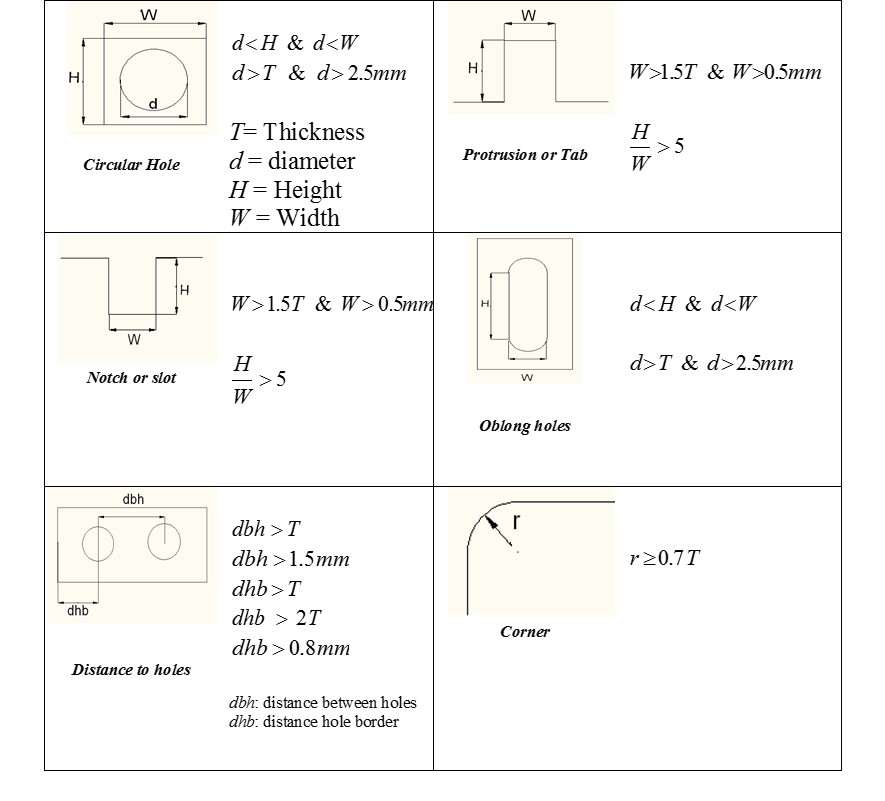
\includegraphics[scale=0.5, angle=-90]{figure-chapterIV/fig4-41}\\
\caption{Manufacturing features with their constraints}
\label{figure4-41}
\end{figure}



This last constraint, Distance between  Holes, has a peculiarity. While the others involve binary relations (e.g $has\_Diameter(h_{1},d)$), this one involves a ternary relation (e.g $distance\_Between\_Holes(h_{1},h_{2},d)$), which is not possible to be expressed in \gls{owl} and is therefore one of the restrictions of this language. In the next section we explain how the heterogeneity approach will help to overcome this issue. 


\section{Extending Ontologies through Heterogeneity}\label{section4.5}

Given that in the previous section, a shortcoming of \gls{owl} was identified during the procedure of trying to represent certain manufacturing restrictions, and in order to provide inferences for it, it is necessary to recall  Fig. \ref{figure3-1} to determine which course of action to take. In the methodology set out there, a branch toward heterogeneity was included. Heterogeneous ontologies has been proposed as a further way to deal with the limitations of certain logics, making available other logics that provide more reasoning power.


In \cite{ramos_hetereogeneous_2012}   we introduced an architecture to deal with the validation of features such as those represented in Fig. \ref{figure4-35}. These in fact correspond to the Distance between holes example mentioned in previous section, and illustrated in Fig. \ref{figure4-41}. That is, there are two holes, $h_{1}$, $h_{2}$, and a restriction of distance $d$ between them . We can represent such a restriction by means of the following ternary relation: $distance\_Between\_Holes(h_{1},h_{2},d)$.  Furthermore, we add a new restriction   called $distance\_Hole\_Border$, which is also mentioned in the literature. These distance features are considered during manufacturing in order to avoid metal deformations when the hole is too close to the border, or when holes are too close to each other as well. 


\begin{figure}
\begin{center}
	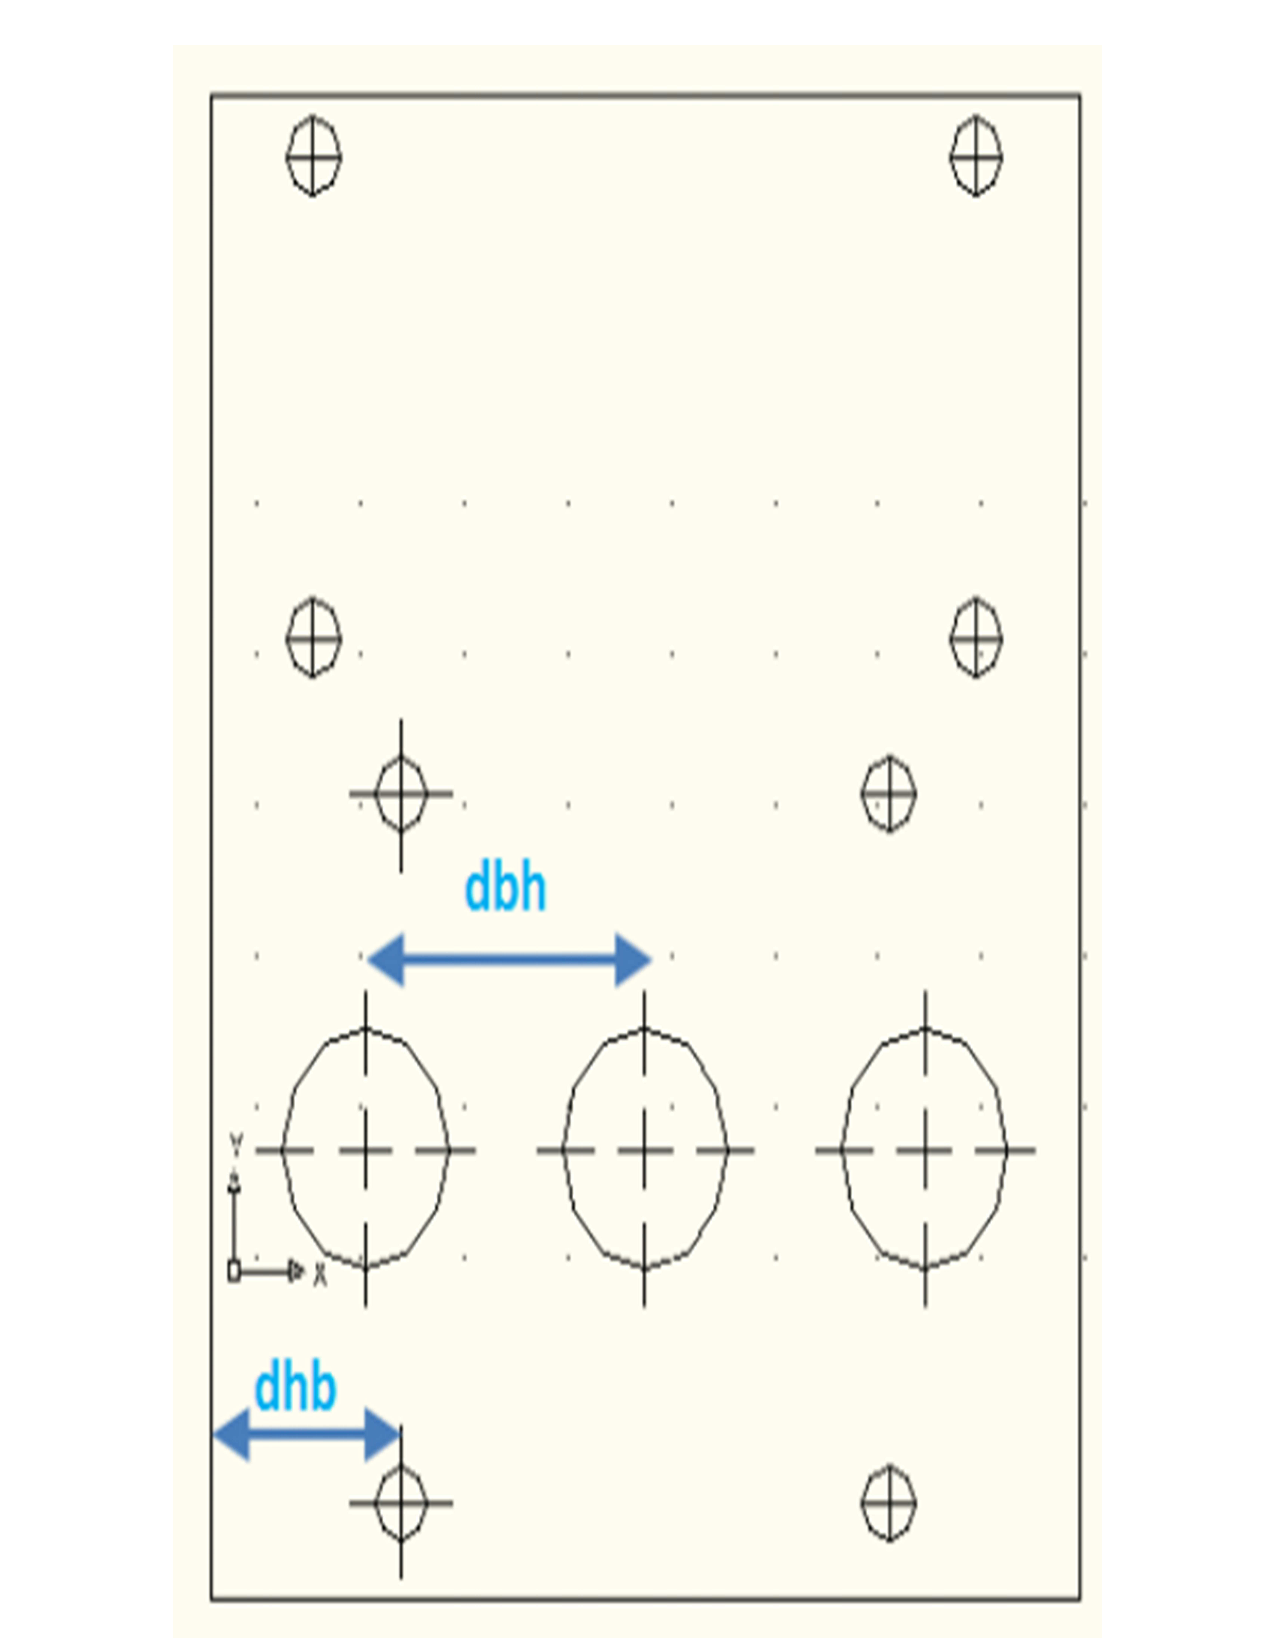
\includegraphics[scale=0.5]{figure-chapterIV/fig4-35}\\
	\caption{Restrictions in Sheet Metal Parts Fabrication  }
	\label{figure4-35}
\end{center}
\end{figure}


Each of these restrictions involves two  instances of the sheet metal issue, and they become related by a valued number restriction. For representing these features, we proceed as follows: in equation \ref{eq4.10}, an intra-feature restriction is present, while in equations \ref{eq4.11} and \ref{eq4.12} inter-feature restrictions are introduced.

\begin{equation}\label{eq4.10}
has\_Diameter(h_{1},d)
\end{equation}

\begin{equation}\label{eq4.11}
distance\_Between\_holes(h_{1}, h_{2}, d)
\end{equation}

\begin{equation}\label{eq4.12}
distance\_Hole\_border(h_{1}, b_{2}, d)
\end{equation}


The restriction described in equation \ref{eq4.10} can be represented in \gls{owl} and conclusions about the quality of the feature itself can be deduced by reasoning. Restrictions expressed in equations \ref{eq4.11} and \ref{eq4.12} can be indirectly expressed in \gls{owl}, but no conclusions about the quality of this design can be obtained from the \gls{owl} model because \gls{owl} reasoning is limited to binary relations, while equations \ref{eq4.11} and \ref{eq4.12} illustrate ternary relations. It is also worth mentioning that the value of these features (dbh and dhb) shown in Fig. \ref{figure4-35} also depend on the materials and other features, for instance thickness. Moreover, we have also avoided mentioning metric units in order to simplify the exposition at this point. This example is an illustration of a type of issue that involves higher predicate arity in a specific task where \gls{owl} expressiveness is insufficient to reach the validation of certain mechanical features. 


To deal with a scenario such as the one previously described, and to fulfill the modeling requirements of engineering, we at least need an ontology language with a higher expressiveness level. But, when we move from \gls{owl} to a more expressive ontology language, we also face the risk of falling into undecidable scenarios. This is a common trade off that has been previously studied and for which frameworks have been proposed. In this vein, if we can precisely divide the scenarios when \gls{owl} is expressive enough for our purposes from the ones where \gls{owl} is not enough, then we can introduce a formalism to represent our requirements and evaluate its decidability level.

Therefore, we propose a heterogeneous architecture to bridge the gap between representing and reasoning over manufacturing requirements in the Semantic Web.  Fig. \ref{figure4-36} presents our architecture. It is a modified view of the architecture presented in \cite{w3c_product_2005}. The main difference is  the inclusion of a heterogeneous layer. Such a layer allows us to face engineering requirements written in different logics. Our architecture includes:  

\begin{enumerate}

\item A Product Ontology (PO) that contains product definitions and features that can be represented in a given language and where conclusions concerning their accuracy can also be obtained.  

\item Exemplifications of this PO that can be performed by introducing specific designs into it.  

\item A heterogeneous bridge for when higher expressiveness with proof capabilities is required.  

\item Quantities, Units and Scale are also included as elements of this architecture, because they are a fundamental aspect in product descriptions. There are links to the Heterogeneous Bridge because we do not want to employ a fixed standard system, but leave open the possibility of assigning the one preferred by the product user.  

\end{enumerate}



Considering the last mentioned aspect related to unit systems, in this case we decide to validate a library of \gls{cad} designs. The features listed in Fig.\ref{figure4-35} could be represented in different metric systems, and even in heterogeneous metric systems (e.g International Metric System, British Metric System). \gls{owl} would not be expressive enough for representing and reasoning on the accuracy of such features. Consequently, in order to simplify the scenario we have considered homogeneous designs at this stage, which means a unique homogeneous measurement system. \gls{hets} and \gls{casl} are the basement of our architecture (See Heterogeneity Building Block\footnote{https://github.com/luisenriqueramos1977/OntoSmart/wiki/Heterogeneity} of Onto\textit{Smart} for a detailed explanation of \gls{hets} and \gls{casl}).

Fig. \ref{figure4-37} shows the \gls{casl} code corresponding to \texttt{My\_Checker} specification. In the upper part, a \gls{sfo} is imported with its terminology into My\_Checker, and    the natural numbers library (Nat). Then, a group of ternary predicates are defined: designDistance, standardDistance and properDistance. Finally, we specify that there will be a proper distance if the design distance is greater than the standard distance.

Fig. \ref{figure4-38} introduces this proof obligation for a set of instances from the \gls{sfo} ontology. There, the \texttt{properDistance} predicate is used to evaluate the values of \texttt{hole\_u1} and \texttt{hole\_u2} from \gls{sfo}. 


\begin{figure}
\begin{center}
	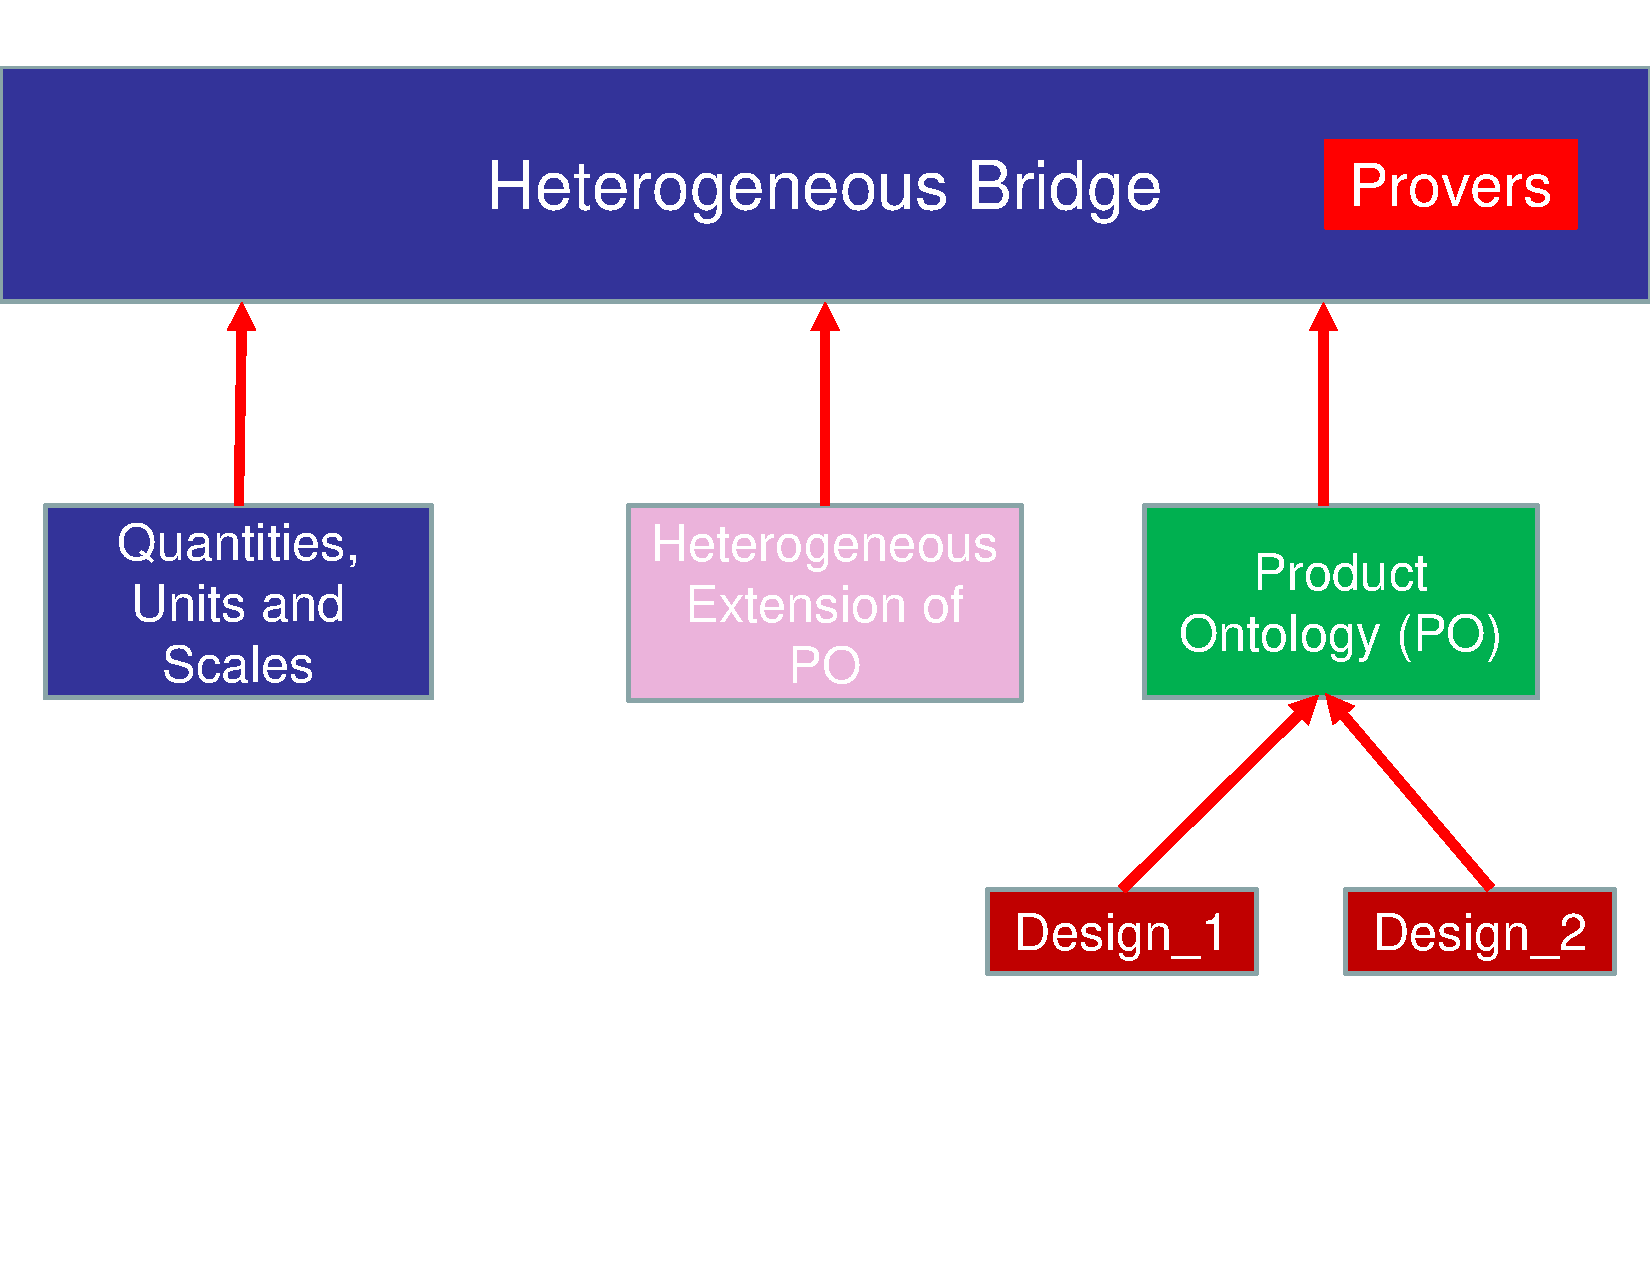
\includegraphics[scale=0.5]{figure-chapterIV/fig4-36.pdf}\\
	\vspace{-10mm}
	\caption{Heterogeneous Ontological Manufacturing Architecture }
	\label{figure4-36}
\end{center}
\end{figure}



\begin{figure}

\begin{center}
	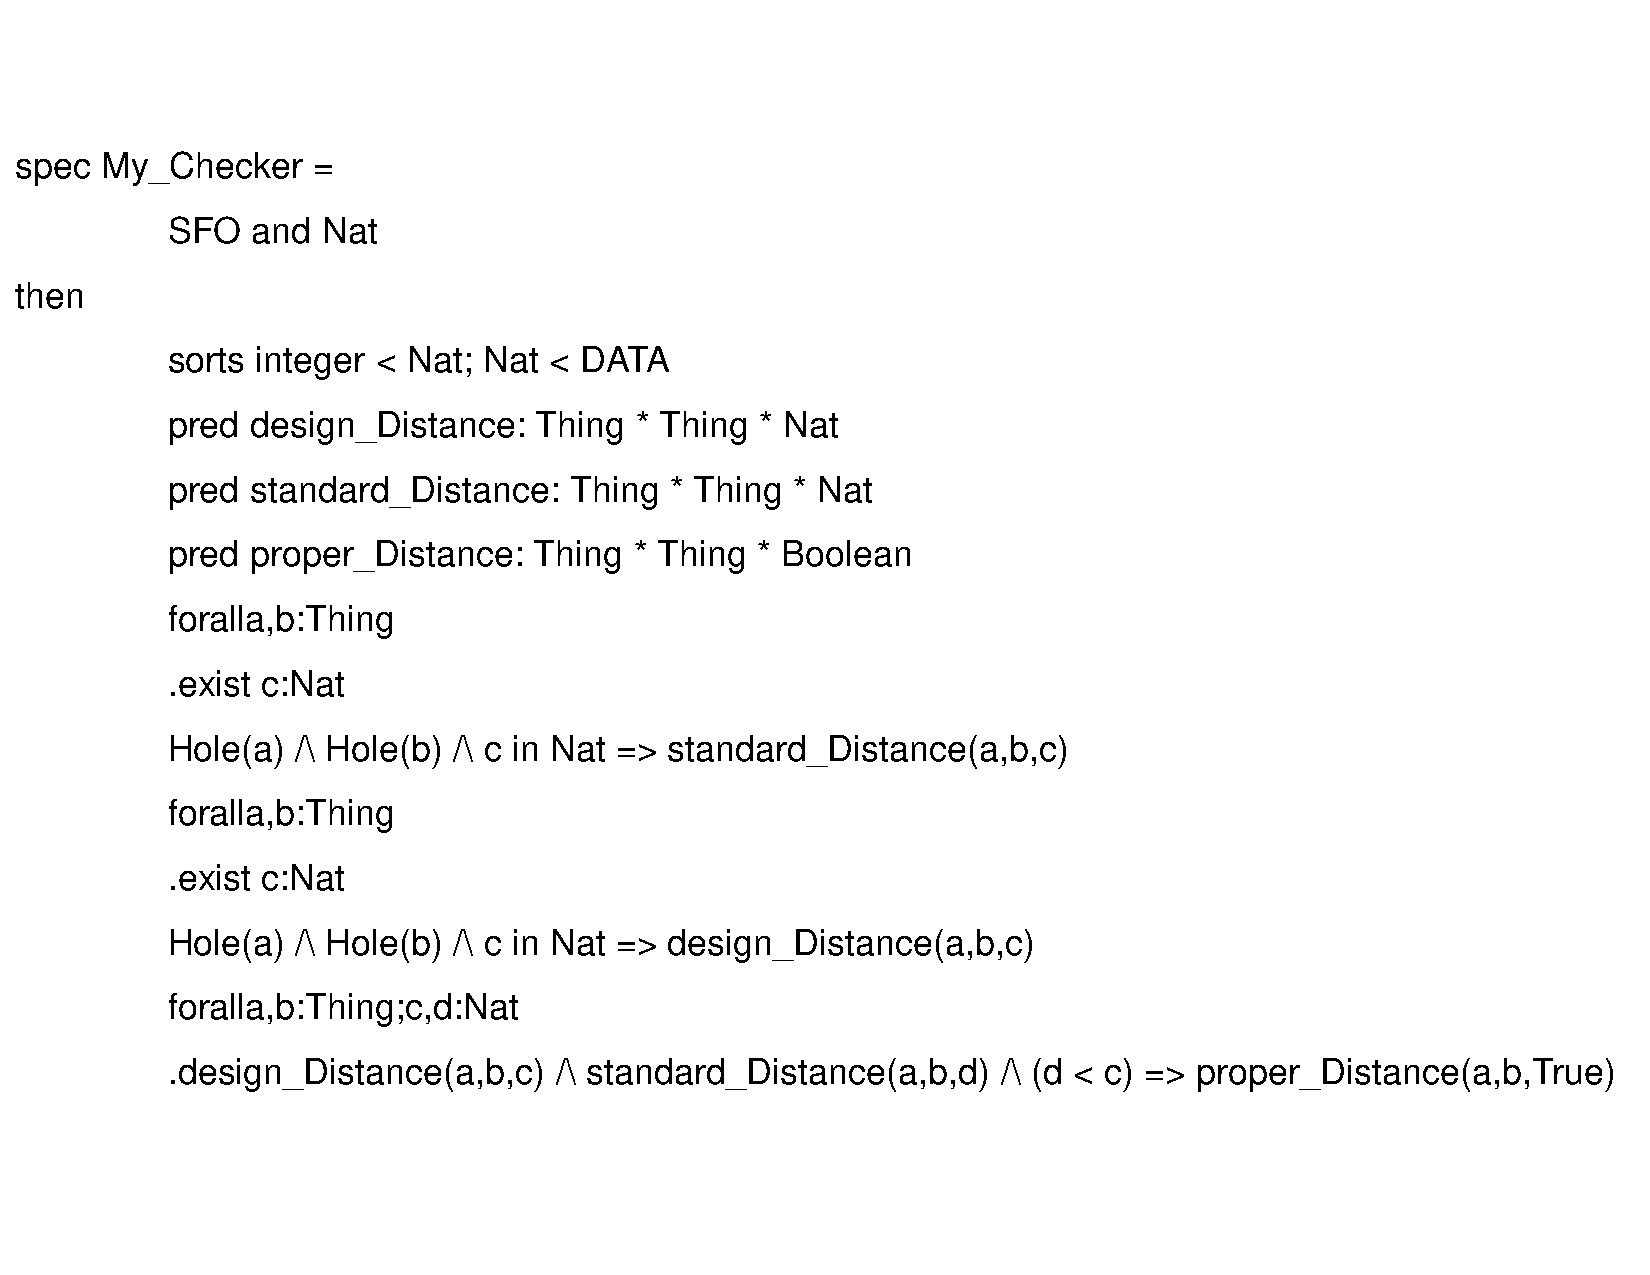
\includegraphics[scale=0.7, angle=90]{figure-chapterIV/fig4-37.pdf}\\
	\caption{Partial View of \texttt{My\_Checker} Spec}
	\label{figure4-37}
\end{center}

\end{figure}


\begin{figure}
\vspace{-50mm}
\begin{center}
	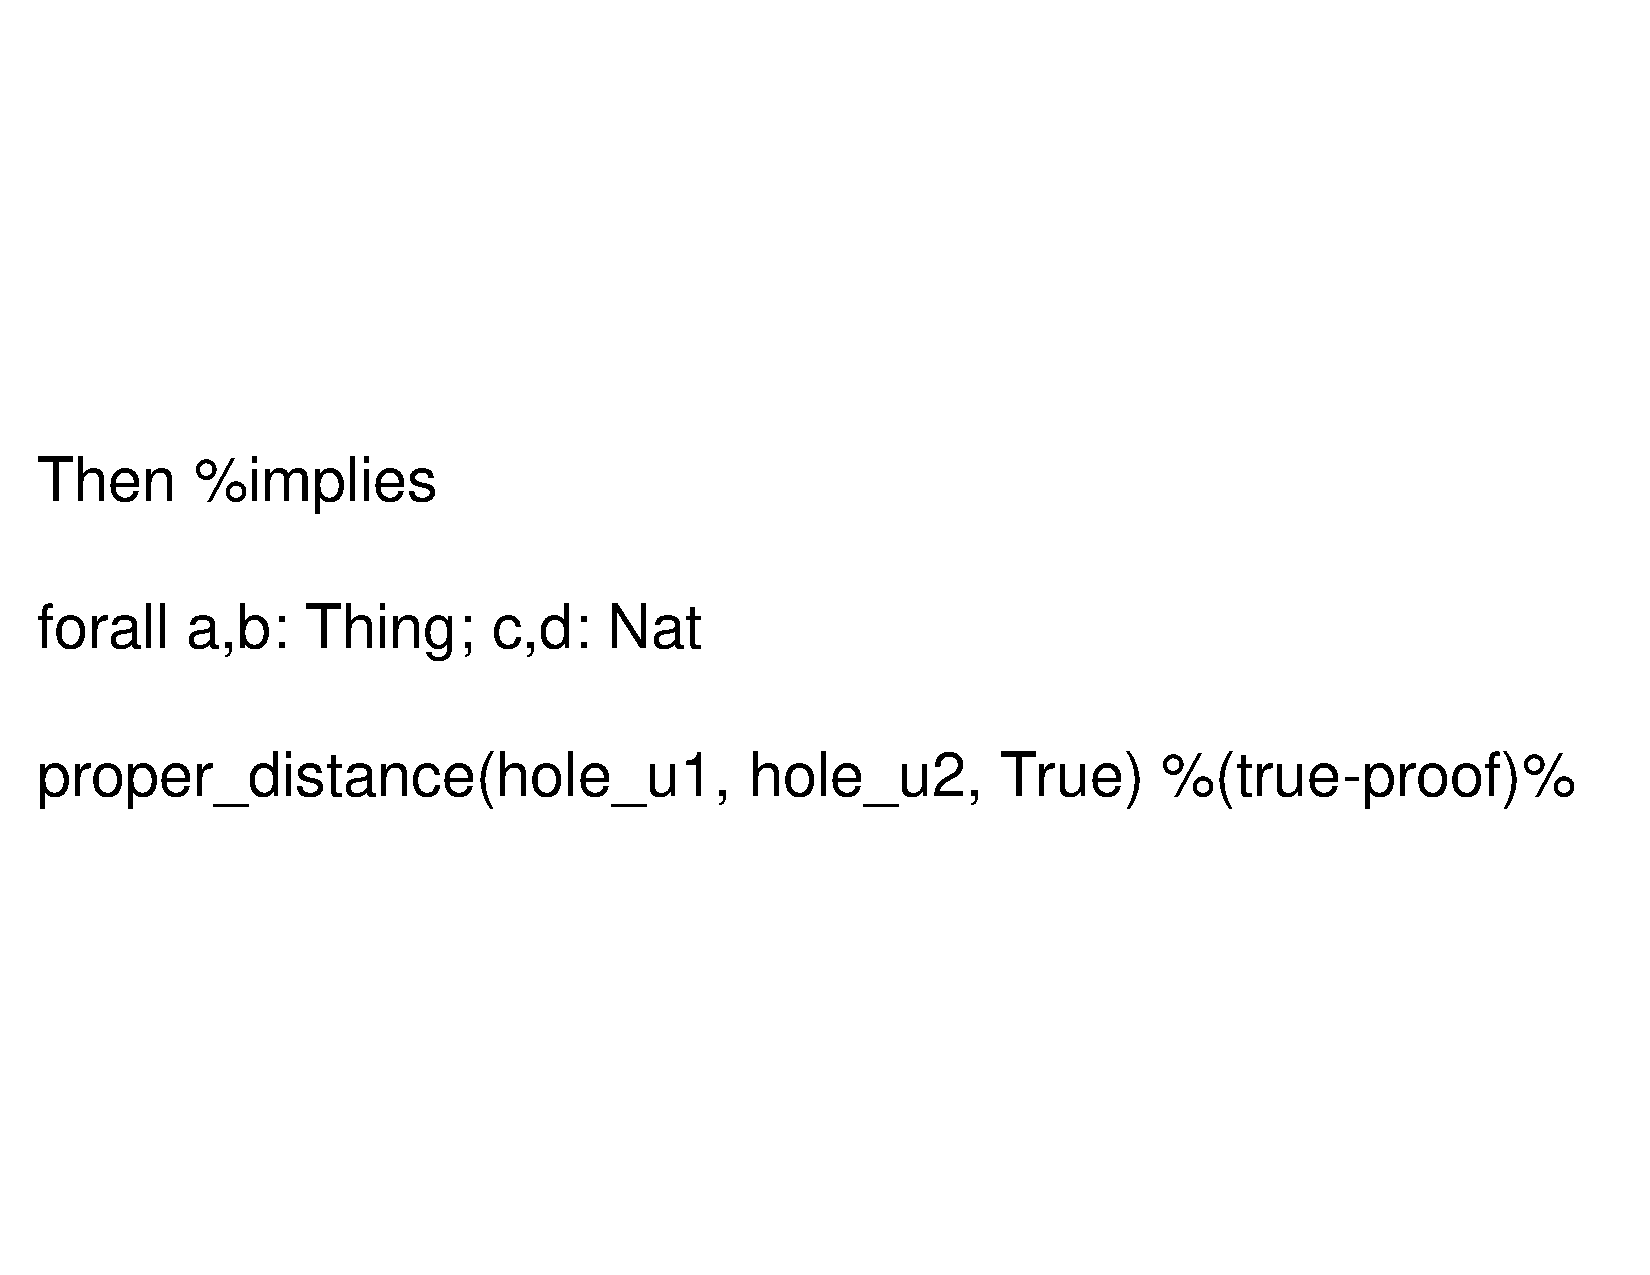
\includegraphics[scale=0.5]{figure-chapterIV/fig4-38.pdf}\\
	\vspace{-80mm}
	\caption{Instantiated  Proof}
	\label{figure4-38}
\end{center}

\end{figure}



\begin{figure}
\begin{center}
	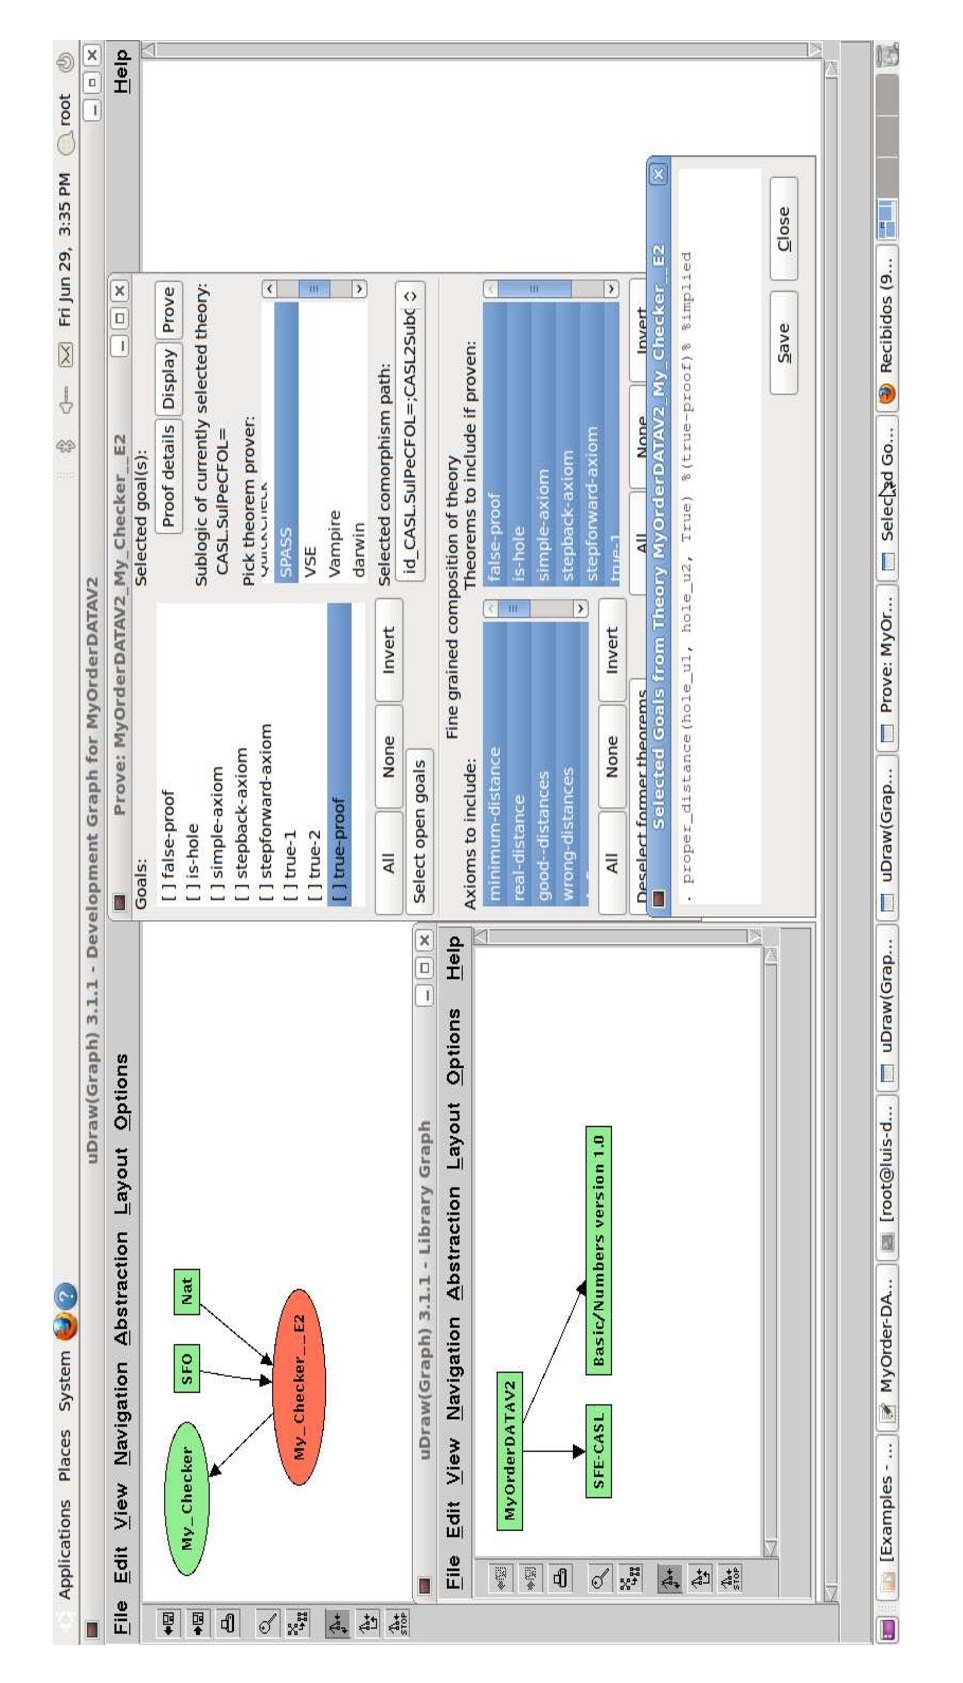
\includegraphics[scale=0.5, angle=270]{figure-chapterIV/fig4-39}\\
	\caption{\texttt{My\_Checker} \gls{hets} view }
	\label{figure4-39}
\end{center}
\end{figure}


After loading the specification in \gls{hets} we obtained the windows shown in Fig. \ref{figure4-39}.  On the left side, at the top and bottom, the development graphic is represented. There, nodes named Nat, \gls{sfo} and \texttt{My\_Checker} correspond to given specifications; such nodes are shown in green color in \gls{hets}. More specifically, Nat comes from the library of Numbers (\gls{casl}), \gls{sfo} comes from the \gls{sfo} (\gls{owl}) and \texttt{My\_Checker} imports both (\gls{sfo} and Nat). The node \texttt{My\_Checker\_E2}, shown in red by \gls{hets}, represents proof obligations. On the right side of the same figure, in the top  view we can observe the axiom to be proved representing the proof obligation. Finally, in the  middle of the  window, there is a list of all axioms present in the specification and the available theorem provers. They are identified as “Axioms to Include” and “Theorems to Include if Proven”.  

To complete our task, the theorem prover SPASS \cite{weidenbach_chapter_2001} was run in proof node to assure the correctness of our instantiation. Fig.\ref{figure4-40} depicts the result, which was proved in this opportunity, confirming that our design complies with the technical requirements.



\begin{figure}
\begin{center}
	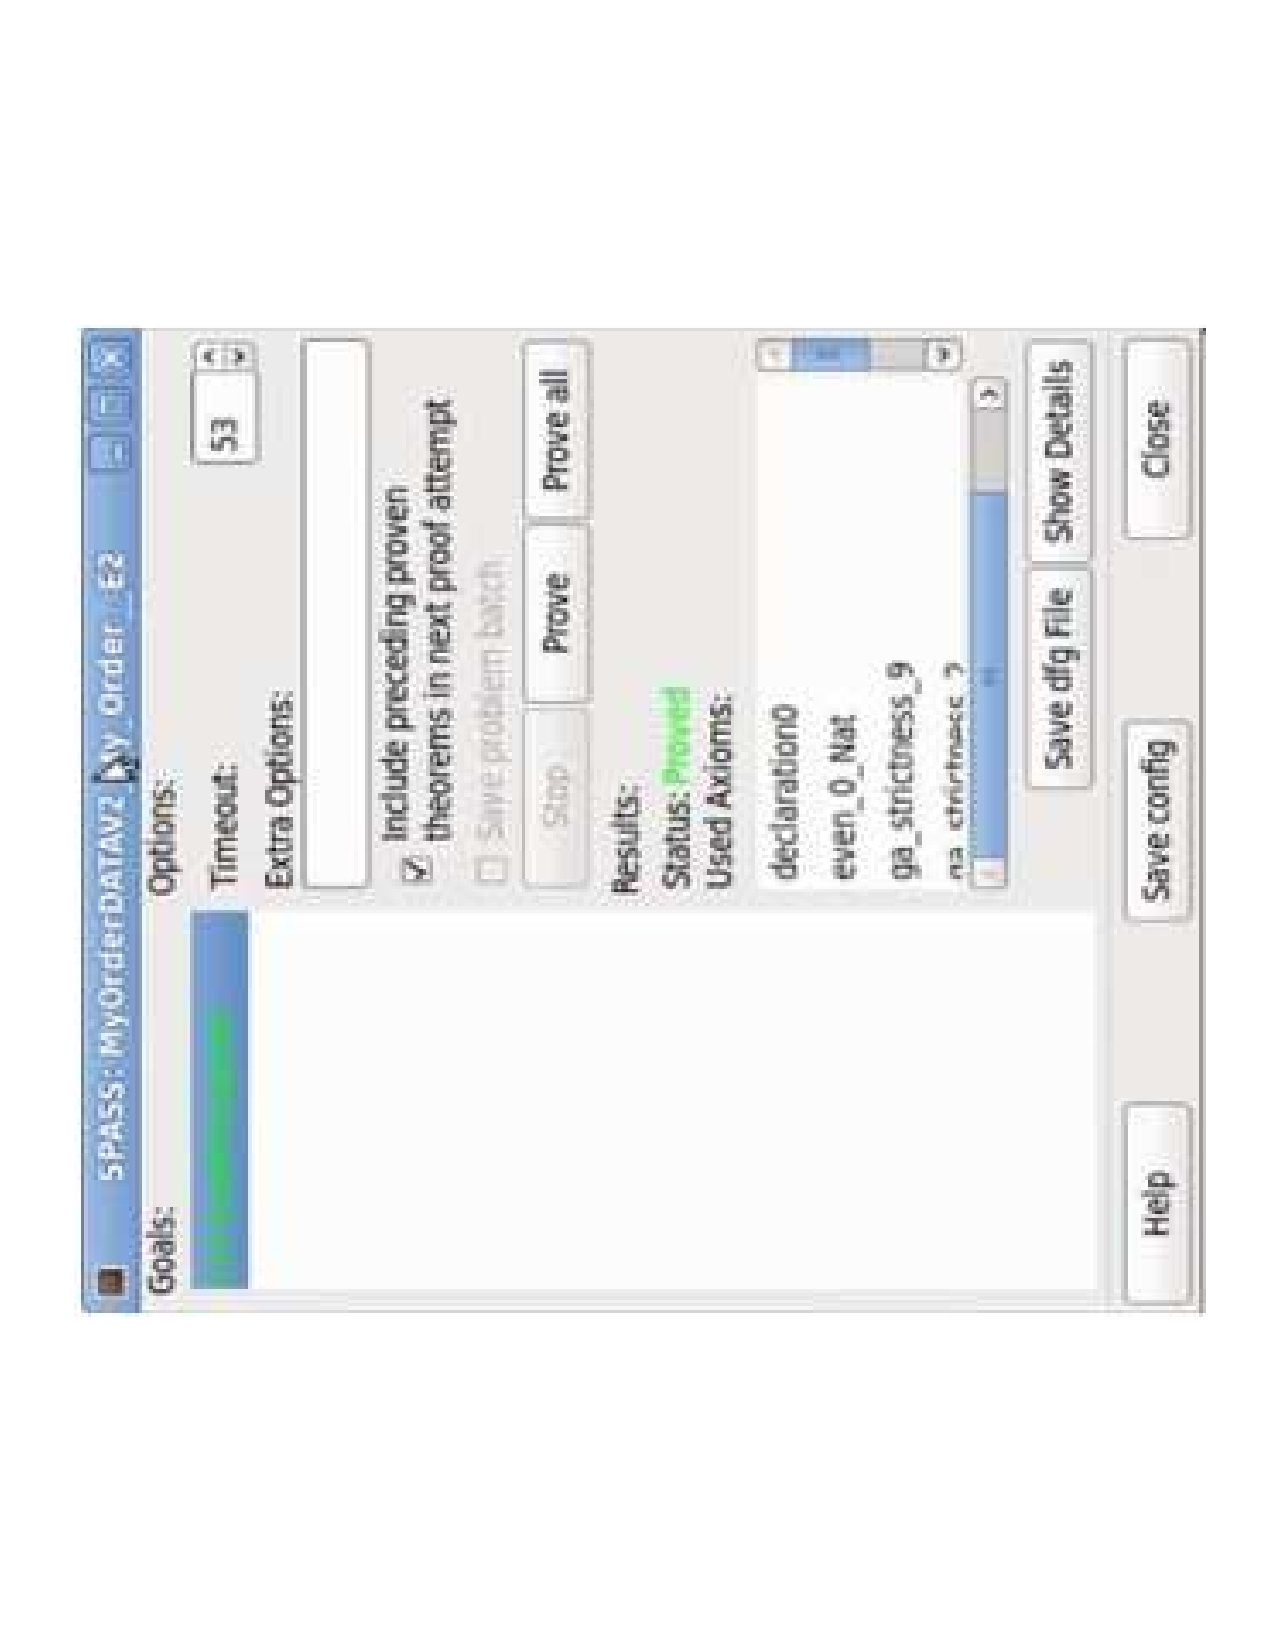
\includegraphics[scale=0.5, angle=-90]{figure-chapterIV/fig4-40.pdf}\\
	\caption{Proof of Sample provided}
	\label{figure4-40}
\end{center}
\end{figure}

This then overcomes the reasoning \gls{owl} restriction, as demonstrated by implementing the architecture proposed in Fig.\ref{figure4-36}.

We have to follow up with the final implementation of the products obtained from the systematic application of the methodology proposed in Fig. \ref{figure3-1}. But in fact, this implementation was carried out progressively from the modularization stage onward. This criterion was captured in our methodology as an \texttt{Implementation} arrow that starts in \texttt{Modularization} and ends in \texttt{Return\_Disp}. In other words, since the very beginning a list of competency questions were defined in Subsection \ref{4.1.2}, and since then we followed a course of action in order to provide answer to such questions. 


Throughout this Section we captured the implementation of the methodology we proposed in Onto\textit{Smart}. Our main motivation for this proposal was the ongoing discussion in ontological engineering which includes topics such as reusability, \gls{ulo}, modularity and heterogeneity. We proposed some specific metrics and methods to serve as criterion in a development workflow. A group of ontologies related with the manufacturing domain was selected because in this domain the manufacturing community has shown interest in Ontological Engineering.  These ontologies passed an evaluation procedure, based in information quality and Competency Questions. Given that no ontology provided answers to all competency questions, we tried to make reusable the knowledge encoded in these ontologies. Our first attempt was using one of the ontologies as an interoperability artifact, however according to this proposed metrics and the obtained results, no upper level ontology was found. This result is worth mentioning because some authors have stated that their ontologies were of upper level, and for us these statements can be questions. Due to these results it was necessary to continue with our methodological workflow, in order to  fulfill our requirement. Whereby some hyper-modules were extracted from the network ontologies under study. The resulting hyper-modules were integrated in an Hyperontology shown in Fig.\ref{figure4-28}. Later, during the implementation phase, the \gls{owl} restrictions as ontology language were evidenced to represent the proposed scenario, therefore it was necessary to proceed with the heterogeneous activities proposed in our methodology. The inclusion of an heterogeneous layer made possible to complete the workflow, and check the restriction in the product shown in Fig.\ref{figure4-36}. With this result we consider to have complete the methodological workflow we proposed.

In next Section we present our conclusion and discussion future work.
%%In the next chapter we will represent and discuss our conclusions.  














